\documentclass[11pt]{article}
\usepackage{geometry}                % See geometry.pdf to learn the layout options. There are lots.
\geometry{a4paper}                   % ... or a4paper or a5paper or ... 
\usepackage{graphicx,tabularx}
\usepackage{amssymb}
\usepackage{amsmath}
\usepackage{epstopdf}
\usepackage{hyperref}
\usepackage{breakurl}
\usepackage{pdflscape}
\usepackage{tikz}
\usetikzlibrary{matrix,arrows,automata,shapes,decorations.pathreplacing}
\usepackage[stable]{footmisc}

%\usetikzlibrary{arrows,decorations.pathmorphing,backgrounds,fit}

\setlength\parindent{0pt}
\DeclareMathOperator*{\argmax}{arg\,max}

\parskip 1mm

\newcommand{\bv}{\begin{verbatim}}
\newcommand{\ev}{\begin{verbatim}}
\newcommand{\var}{\mbox{Var}}
\newcommand{\sqend}{\hfill $\square$}

\DeclareGraphicsRule{.tif}{png}{.png}{`convert #1 `dirname #1`/`basename #1 .tif`.png}

\title{369 Computational Science}
% Maximisation, matrix decomposition, probability, inference, simulation, bioinformatics and phylogenetics}
\author{Compiled, collated and written by David Welch\\ 
Sections \ref{sec:intro}-\ref{sec:leastsquares} are based on slides by Georgy Gimel'farb,  sections 16--18 are\\ based on the book Biological Sequence Analysis by Durbin et al. 2010. \\ Other sections are incompletely referenced so \\ presence in these notes is no claim of authorship.}
\date{2019}                                           % Activate to display a given date or no date
\begin{document}
\maketitle

%\section*{What is and what is not in the exam}
%
%Nearly all the material we have covered in lectures is examinable. All the major parts of the course that are not examinable have been removed from these notes.  A few bits listed below have been left in but won't be directly tested in the exam.
%
%\begin{itemize}
%\item Sections 11-11.4 Review of probability (assumed you know this so left here for revision)
%\item Don�t need to memorise functional form for common distributions in Sec 11.5
%\item Formulae for calculating Akl and Ek(b) without imputing seqeunces in Baum-Welch in Sec 18.7
%\item Mathematical definition of ultrametric and additive distances in 19.2 and 19.3
%\item Formulae in Neighbour-Joining algorithm in Sec 19.4
%\end{itemize}

\tableofcontents
\newpage





\section{Introduction} \label{sec:intro}
This  course is aimed at introducing computer scientists to uses of computers and computational techniques in other areas of science.    The number of ways that computers are used in the sciences are many, varied and often extremely sophisticated.   The focus of this course will be  on  ``computational science'' which involves constructing mathematical models that can be simulated, analysed and solved using computational methods.  

The course is split into two parts:  in the first 3-4 weeks, we'll look at techniques for finding the roots of equations, solving systems of linear equations and decomposing matrices.  These techniques are basic to areas of research known as computational engineering, numerical analysis and applied linear algebra.  

In the remaining 8-9 weeks, we'll turn to computational biology, with a focus on bioinformatics and phylogenetics.  There, we see how a wide range of computational and mathematical techniques have revolutionised an area of science and allowed us to  analyse and interpret huge amounts of genetic data. This area of study has helped us better understand, among other things,  the basic workings of life,  our evolutionary  history, the causes of inherited diseases and the spread of infectious disease. 

From a computational point of view, computational biology is a fascinating and active area of research.  The techniques we'll study in this part of the course include stochastic and probabilistic modelling,  simulation, dynamic programming, estimation and inference.

CS 369 is more mathematical than many CS courses. This is unavoidable given the subject matter.   We assume that students have some background in discrete mathematics (matrices, graphs, linear equations) and continuous mathematics (functions, derivatives, integration), and an understanding of basic probability (discrete and continuous random variables, expectation, conditional probability) .    However, we recognise that students come to this course from a variety of  backgrounds so will provide explanations from quite a basic level in most cases.  We do assume that students have a solid foundation in programming in one of Java, C++, Python, Matlab or R.





\section{Mathematical modelling and why we need computers}
\label{sec:why}
Mathematical models attempt to precisely describe a system in order to better understand it.  A model is usually based on observing the system and is often structured to answer a particular question. It is not an exact replica of the system and is not merely a description of the observations.  Recorded observations of the system are known as data.   Coupled with data, the model allows us to infer unobserved properties of the model (such as model parameters) and predict future outcomes.  Careful comparison of outcomes predicted by the model with data (actual outcomes) tell us how accurate the model is and where it needs to be refined.


This process of modelling and observation has, arguably, been used for thousands of years and certainly for hundreds.  The complexity of the models we create and study is somewhat determined by our ability to interpret and ``solve'' them.  Before computers, we were largely limited to using models that were analytically tractable --- that is, models for which closed form  solutions could be found  --- or for which good approximations could be made by hand.  Our ability to fit models to data was severely  limited by our human limitations of collecting, storing and processing information by hand.  

With the advent of computers, both of these limitations have eased considerably.  It is now possible to collect and store massive amounts of data.  For example, Genbank, which stores genetic nucleotide sequences  contains over 204 billion nucleotide bases in more than 189 million sequences as at the end of 2015, while CERN's Large Hadron Collider produces 30 PB ($=30 \times 10^6$ GB) of data annually.  And fast computers allow us process this data and  to make  almost  arbitrarily good approximations to models that are far more complex than could be tackled by hand.  

However, even with all the data and computing power in the world we need to be careful to propose useful models  and tackle them with efficient techniques if we are to make progress in answering questions that interest us.  Bad models, bad data or bad computational techniques could all derail our quest for understanding.  In this course, we aim to teach good computational techniques and give some insight into some basic modelling and data analysis techniques that will help to tackle and answer a range of interesting questions.

\subsection{Why we need to be clever about our computing}

Mathematical problems can be classed into problems that are {\em well-posed} and {\em ill-posed}.  A problem is {\em well-posed} if 
\begin{enumerate}
\item A solution exists
\item the solution is unique
\item A small change in the initial condition induces only a small change in the solution
\end{enumerate}
A problem that is not well-posed is ill-posed.

We are interested in the last criterion which can be termed {\em sensitivity}.  Suppose our problem has inputs $x$ and has a solution (or output) $y$.  An {\em insensitive} or {well-conditioned} problem is when a change in $x$ causes a change in $y$ that is of similar relative size.  A {\em sensitive} or {\em ill-conditioned} problem is one in which the change in solution/output can be  large relative the the change in input.  

Based on this idea, define the {\em condition number} by 
\[ cond = \frac{|\mbox{relative change in solution}|}{|\mbox{relative change in input data}|} = \left|\frac{\Delta y/y}{\Delta x/x}\right |. \]
Thus a problem is {\em ill-conditioned} is $cond \gg 1.$

{\bf Example}:  what is the condition number when we evaluate a function $y = f(x)$ at an approximation of $x$, $\hat x = x+ \Delta x$, rather than at the true value $x$?

{\bf Solution}: \[ cond = \left|\frac{\Delta y/y}{\Delta x/x}\right | = \left|\frac{f(x+\Delta x) - f(x)/f(x)}{\Delta x/x}\right | = \left|\frac{f(x+\Delta x) - f(x)}{\Delta x} \frac {x}{f(x)}\right | \approx \left | \frac{x f'(x)}{f(x)} \right |.  \]
So, depending on the function $f$ and the input $x$, we could get very large condition numbers. \sqend

{\bf Example}:  What is the condition number for the functions $f(x) = x^n$ and $f(x) = e^x$?

{\bf Solution}: From above, the condition number is \[ cond \approx \left | \frac{x f'(x)}{f(x)} \right |. \]  When $f(x) = x^n$, $f'(x) = n x^{n-1}$, so  \[ cond =  \left | \frac{x f'(x)}{f(x)} \right | = \left | \frac{x . n x^{n-1}}{x^n} \right | = \left | \frac{ n x^{n}}{x^n} \right |  = |n|.\]
So as the degree of the polynomial increases, the problem becomes increasingly ill-conditioned.


Similarly, when $f(x) = e^x$, $f'(x) = e^x$ so \[ cond =  \left | \frac{x f'(x)}{f(x)} \right | = \left | \frac{x .e^x}{e^x} \right |  = |x|.\]
In this case, the condition number depends on the input argument, $x$.  If $x$ is very large, the problem can be considered ill-conditioned.   \sqend




What does this mean for computation?  In nearly all our computations, we will replace  exact formulations with approximations.  For example,  we approximate continuous quantities with discrete quantities, we are limited in size by floating point representation of numbers which often necessitates rounding or truncation and introduces (hopefully) small errors.  If we are not careful, these error will be amplified within an ill-conditioned problem an produce inaccurate results.

This leads us to consider the {\em stability}   and {\em accuracy} of our algorithms.   

An algorithm is {\em stable} if the result is relatively unaffected by perturbations during computation.  This is similar to the idea of conditioning of problems.  

An algorithm is {\em accurate} is the competed solution is close to the true solution of the problem.  Note that a stable algorithm could be inaccurate. 

We seek to design and apply stable and accurate algorithms to find accurate solutions to well-posed problems (or to find ways of transforming or approximating ill-posed problems by well-posed ones).



\section{Approximating a function by a Taylor series}

First, a little notation.  A real-valued function  $f:\mathbb R \to \mathbb R$ is a function  $f$ that  takes a real number argument, $x  \in \mathbb R$ ,and returns a real number, $f(x) \in \mathbb R$. We write $f'(x)$ to denote the derivative of $f$, so $f'(x) = \frac {df}{dx}$, and $f''(x)$ is the second derivative (so  $f'(x) = \frac{d}{dx}(\frac {df}{dx}) = \frac{d^2 f}{dx^2}$) and $f^{(k)}(x)$ is the $k$th derivative of $f$ evaluated at $x$.

As we have just seen, simply evaluating a real valued function can be prone to instability (if the function has a large condition number).  For that reason, approximations of functions are often used.   The most common method of approximating the real-valued function $f:\mathbb R \to \mathbb R$  by a simpler function is to use the Taylor series representation for $f$.  

The Taylor series has the form of a polynomial where the coefficients of the polynomial are the derivatives of $f$ evaluated at a point. So long as all  derivatives of the function exists at the point $x = a$, $f(x)$ can be expressed in terms of of the value of the function and it's derivatives at $a$ as:
\[ f(x) = f(a) + (x-a)f'(a) + \frac{(x-a)^2}{2!}f''(a) + \ldots + \frac{(x-a)^k}{k!}f^{(k)}(a) + \ldots \]
This can be written more compactly as 
\[ f(x) = \sum_{k = 0}^{\infty} \frac{(x-a)^k}{k!}f^{(k)}(a), \]
where $f^{(0)} = f$ and $0! = 1$ by definition.  

This is known as the {\em Taylor series} for $f$ about $a$.  It is valid for $x$ ``close'' to $a$ (strictly, within the ``radius of convergence'' of the series).   When $a = 0$, the Taylor series  is known as a {\em Maclaurin series}.

This is an infinite series (the sum contains infinitely many terms) so cannot be directly computed.  In practice, we truncate the series after $n$ terms to get  the {\em Taylor polynomial of degree $n$} centred at $a$, which we denote $\hat f_n(x;a)$:
\[ f(x) \approx \hat f_n(x;a) = \sum_{k = 0}^{n} \frac{(x-a)^k}{k!}f^{(k)}(a). \]
This is an approximation of $f$ that can be readily calculated so long as the first $n$ derivatives of $f$ evaluated at $a$ can be calculated.  The approximation can be made arbitrarily accurate by increasing $n$.  The quality of the approximation also depends on the distance of $x$ from $a$ --- the closer $x$ is to $a$, the better the approximation.

{\bf Example}: Find the Taylor approximation of $f(x)=\exp(x) =  {e}^x$ for values of  $x$ close to 0. 

{\bf Solution:} The $k$th derivative of  $f(x) = e^x$ is simply $e^x$ for all $k$.  Since we want values of $x$ close to 0, find the Taylor series about  $a = 0$ (the Maclaurin series).   Then 
 
\[ \widehat{f}_n(x;0) = 1 + \frac{x}{1!} + \frac{x^2}{2!} + \frac{x^3}{3!} + \cdots = \sum\limits_{k=0}^{n}\frac{x^k}{k!} \]

 This  series converges to $\mathrm{e}^x$ everywhere: $\lim\limits_{\rightarrow\infty} \widehat{e}_n(x)= e^x$.  The quality of the approximation for various values of $n$ and $x$ are studied in the table below.
\[
\begin{array}{r|ccccc|c}
n & 1 & 2 & 3 & 4 & \ldots & \textsf{true value }e^x\\ \hline
\widehat{f}_n(x=1;0) & 2.0000 & 2.5000 & 2.6667 & 2.7083 & \ldots & {2.7183}\\
\textsf{\scriptsize Relative error} & 0.26 & 0.08 & 0.019 &  0.0037 & &\\ \hline\hline
\widehat{f}_n(x=2;0) & 3.0000 & 5.0000 & 6.3333 & 7.0000 & \ldots  & {7.3891}\\
\textsf{\scriptsize Relative error} & 0.59 & 0.32 & 0.14 &  0.053 & &\\ \hline
\end{array}
\]

Notice that the error is smaller for $x$ close to $a$ and decreases as $n$, the number of terms in the polynomial increases.   \sqend


\section{Finding the roots of equations}

Given a real valued function $f:\mathbb R \to \mathbb R$,  a fundamental problem is to find the values of $x$ for which $f(x) = 0$.  This is known as finding the roots of $f$.  The problem crops up again and again and many problems can be reformulated as this problem.  For example, if the trajectory of one object is described by $h(x)$, while another object has trajectory $g(x)$, then the two objects intercept one another exactly when $f(x) = g(x) - h(x) = 0. $

Another common application is when we wish to find the minimum or maximum value that a function takes.  We know from basic calculus that if $f$ is the derivative of some function $F$, then $F(x)$ takes its  maximum or minimum values when $f(x) = 0$.  Thus finding the maximum value of $F$ is a matter of finding the roots of $f$.  

We will consider two simple yet effective root finding algorithms.  The bisection method and Newton's method.  In both cases, we assume that $f:\mathbb R \to \mathbb R$ is continuous.

\subsection{Bisection method}

We want to find $x^*$ such that $f(x^*) = 0$.  Let $\mathrm{sign}(f(x)) = -1$ if $f(x) < 0$ and $\mathrm{sign}(f(x)) = 1$ if $f(x) > 0$.  The bisection method proceeds as follows:

\begin{itemize}
\item {\bf Initialise:} Choose initial guesses $a, b$ such that $\mathrm{sign} f(a) \ne\mathrm{sign} f(b)$
\item {\bf Iterate} until the absolute difference $ |a-b| \approx 0$
\begin{itemize} 
\item Calculate $c=\frac{a+b}{2}$
\item If $\mathrm{sign} f(a) =\mathrm{sign} f(c)$, then $a\leftarrow c$; otherwise $b\leftarrow c$
\end{itemize}
\end{itemize}

The method provides slow but sure convergence.
\begin{figure}[htbp]
\includegraphics[width=4in]{figures/bisectionIdea.jpg}
\caption{The idea behind the bisection method. Here, $\mathrm{sign} f(a) =\mathrm{sign} f(c)$ so at the next iteration we will set $a \leftarrow c$. The algorithm stops when $a$ and $b$ are sufficiently close to each other.}
\end{figure}

\subsection{Newton's method}

This method is also known as the Newton-Raphson method and is based on the approximation first two terms of the Taylor series expansion.  Recall that we want to find $x$ such that $f(x) = 0$. From the first two terms of the  Taylor series of $f(x)$, we know that  $f(x)  \approx f(a) + (x - a) f'(a)$.  If $f(x)$ is zero, then the expression on the right hand side to 0 and solve for $x$ to get  
\[ f(a) + (x - a) f'(a) = 0 \implies  x = a - \frac{f(a)}{f'(a) }.\]
We can treat this iteratively, starting at $x_0$, and finding $x_{i+1} = x_i - \frac{f(x_i)}{f'(x_i) }$.  This leads to the algorithm:
\begin{itemize}
\item {\bf Initialise:} Choose $x_0$ as an initial guess.
\item {\bf Iterate} until the absolute difference $\vert x_i-x_{i-1} \vert \approx 0$
\begin{itemize} 
\item Set $x_{i+1} = x_i - \frac{f(x_i)}{f'(x_i) }.$
\end{itemize}
\end{itemize}

{\bf Example}: $f(x) = x^2 - 2$.

{\bf Solution}:  $f'(x) = 2x$ so 
\[
x_{i+1} =  x_i - \frac{f(x_i)}{f'(x_i) } = x_i - \frac{x_i^2 - 2}{2x_i} = \frac{x_i}2 + \frac1{x_i}.
 \]
See slide for example starting at $x_0 = 0.5$. \sqend


Compare with bisection method: Start at $a = 1/2$ and $b = 2$ to get to $a = 1.34375$ and $b = 1.4375$ at the fifth step.  This produces an absolute error of $0.02688$ or 1.9\%.  The absolute error in the Newton case is 0.00020 which is 2 orders of magnitude smaller.

\begin{figure}[htbp]
\includegraphics[width=4in]{figures/NewtonIteration.jpg}
\caption{The idea behind the Newton's method. Starting at $x_n$, we find the tangent line (red) and calculate the point it intercepts the $x$-axis.  This point of intercept is $x_{n+1}$.  }
\end{figure}

%%\notinexam{
There are, of course, many other root finding methods.  We list a few of them here (not examinable).

 Secant method (\url{http://en.wikipedia.org/wiki/Secant\_method}):
\begin{itemize}\setlength{\itemsep}{0pt}
\item Newton's method with a finite difference instead of the derivative
\item Neither computation, nor existence of a derivative is required 
\item However, the convergence is slower (approximately, $\alpha=1.6$)
\end{itemize}
False position method (\url{http://en.wikipedia.org/wiki/False\_position\_method}):
\begin{itemize}\setlength{\itemsep}{0pt}
\item Always retains one point on either side of the root 
\item Faster than the bisection and more robust than the 
secant method
\end{itemize}
Muller's method  (\url{http://en.wikipedia.org/wiki/Muller's\_method}):
\begin{itemize}\setlength{\itemsep}{0pt}
\item Quadratic (instead of linear) interpolations
\item Faster convergence than with the secant method
\item Roots may be complex (in addition to reals)
\end{itemize}
%%}%end not in exam
\newpage

\section{Numerical linear algebra}

Numerical linear algebra is one of the cornerstones of modern mathematical modelling.  Topics as important as solving systems of ordinary differential equations (arising in engineering, economics, physics, biotech, etc),  to network analysis (telecoms, sociologic, epidemiology), internet search, data mining and many more rely on linear algebra.  

These days, applied linear algebra and numerical linear algebra are virtually interchangeable --- problems of all sizes are routinely solved numerically and rely on a wealth of mathematical and computational insight.  

We'll start out with a brief review of topics that you should be somewhat familiar with.


\subsection{Review}

Let $\mathbf{a}=\left[\begin{array}{c}a_1\\ \vdots \\ a_n\end{array}\right]$    
$\mathbf{b}=\left[\begin{array}{c}b_1\\ \vdots \\ b_n\end{array}\right]$ be vectors.  The {\em inner} or {\em dot product} of $\mathbf{a}$ and $\mathbf{b}$  is 
the scalar $c=\mathbf{a}\bullet\mathbf{b} \equiv \mathbf{a}^{\mathsf{T}}\mathbf{b} =\sum\limits_{i=1}^n a_i b_i$. 
The dot product is also called {\em multiplication} of vectors.

The {\em norm} or {\em magnitude} of a vector $\mathbf a$ is  $||\mathbf a|| = \sqrt{a \cdot a} =  \sqrt{\mathbf a^{\mathsf T} \mathbf a} = \sqrt{a_1^2 + \ldots a_n^2}$.

The {\em product} of an $m \times n$ {matrix} 
$\mathbf{A} = \left[ \begin{array}{ccc} A_{11}& \ldots & A_{1n}\\ \vdots &\ddots &\vdots \\ A_{m1}& \ldots &A_{mn} \end{array}\right]$
and an $n\times 1$ ($n$-dimensional) {vector} $\mathbf{x}=\left[\begin{array}{c}x_1\\\vdots\\x_n\end{array}\right]$ is
the $m$-dimensional vector $\mathbf{y}=\mathbf{Ax}$ with the elements $y_i=\sum\limits_{j=1}^m A_{ij}x_j$.

The {\em product} of a $k \times m$ matrix $\mathbf{A}$ and an $m \times n$ {matrix} $\mathbf{B}$ is
the $k \times n$ matrix $\mathbf{C}=\mathbf{AB}$ with the elements $C_{ij}= \sum\limits_{\alpha=1}^{m}A_{i,\alpha}B_{\alpha,j}$

The {\em outer product} of an $m$-dimensional  vector $\mathbf a$ with an $n$-dimensional vector $\mathbf b$ is the $m \times n$ matrix 
\[
\mathbf{a}\mathbf{b}^{\mathsf{T}}\equiv
\left[\begin{array}{c}a_1\\ a_2 \\ \vdots \\ a_m\end{array}\right]
\left[\begin{array}{cccc}b_1&b_2&\ldots&b_n\end{array}\right] =
\left[\begin{array}{cccc}a_1b_1 & a_1b_2 & \ldots & a_1b_n\\
                                          a_2b_1 & a_2b_2 & \ldots & a_2b_n\\
                                          \vdots    & \vdots     & \ddots & \vdots \\
                                          a_mb_1 & a_mb_2 & \ldots & a_mb_n
                                          \end{array}\right]
\] 

The {\em identity matrix} of size $n$, $\mathbf I_n$, is the $n \times n$ matrix with $(i,j)$th entry = 0 if $i \ne j$ and $1$ if $i = j$.  

The {\em inverse} of a square matrix $\mathbf A$ of size $n$ is the square matrix $\mathbf A^{-1}$ such that $\mathbf{AA}^{-1} = \mathbf I_n = \mathbf A^{-1}\mathbf A$. When such a matrix exists, $A$ is called {\em invertible} or {\em non-singular}. $\mathbf A$ is {\em singular} if no inverse exists.  Finding the inverse of $\mathbf  A$ is typically difficult.

The {\em determinant} of  an $n \times n$ matrix $\mathbf A$, written $det(\mathbf A) = \left| \begin{array}{ccc} A_{11}& \ldots & A_{1n}\\ \vdots &\ddots &\vdots \\ A_{n1}& \ldots &A_{nn} \end{array}\right|$, is given by a somewhat complex formula that we need not reproduce here (look it up at  \url{http://en.wikipedia.org/wiki/Determinant}).  For $n= 2$, $det(A)  = A_{11} A_{22} -  A_{21} A_{12}$.  For $n= 3$, $det(A)  = A_{11}A_{22}A_{33} - A_{31}A_{22}A_{13} + A_{12}A_{23}A_{31} - A_{32}A_{23}A_{11} + A_{13}A_{21}A_{32} - A_{33}A_{21}A_{12}$.

{\bf Example}: Find the determinant of $\mathbf  A = \left(\begin{array}{ll}3 & 5\\1&-1\end{array}\right) $.

{\bf Solution}: From above, $det(\mathbf A) = |\mathbf A| = 3 . {-1}  - 1.5 = {-3} -5 = -8$. \sqend

It is worth recalling a few properties of the determinant (as listed on the wiki page): 
\begin{itemize}
\item $det(\mathbf I) = 1$ 
\item $det(A^T) = det(A)$ (transposing the matrix does not affect the determinant) 
\item $det(A^{-1}) = \frac{1}{det(A)}$ (the determinant of the inverse is the inverse of the determinant)
\item For $A, B$ square matrices of equal size, $det(AB) = det(A)det(B)$
\item $det(cA) = c^n\, det(A)$ for any scalar $c$
\item If $A$ is triangular (so has all zeros in the upper or lower triangle) then $det(A) = \prod_{i = 1}^n A_{ii}$.
\end{itemize}


An {\em eigenvector} of the square matrix $\mathbf A$ is a non-zero vector $\mathbf e$ such that $\mathbf A \mathbf e = \lambda \mathbf e$ for some scalar $\lambda$.  $\lambda$ is known as the {\em eigenvalue} of  $\mathbf A$  corresponding to $\mathbf e$.  Note that $\lambda$ may be 0.   So the effect of multiplying $e$ by $A$ is simply to scale $e$ by the corresponding scalar $\lambda$.  

The determinant can be used to find the eigenvalues of $\mathbf A$:   they are the roots of
the {\em characteristic polynomial} $p(\lambda) = \det(\mathbf{A }- \lambda\mathbf{I}_n)$
where $\mathbf{I}_n$ is the identity matrix.


{\bf Example}: Find the eigenvalues of $\mathbf  A = \left(\begin{array}{ll}3 & 5\\1&-1\end{array}\right) $.

{\bf Solution}: We need to solve $p(\lambda) = \det(\mathbf{A }- \lambda\mathbf{I}_2) = 0$. 
\[ \begin{array} {lcl}  | \mathbf{A }- \lambda\mathbf{I}_2 |  &= &   \left\vert \left(\begin{array}{ll}3 & 5\\1&-1\end{array}\right) - \lambda  \left(\begin{array}{ll}1 & 0\\0&1\end{array}\right) \right\vert \\
& = &   \left\vert \begin{array}{ll}3-\lambda & 5\\1&-1 - \lambda\end{array}  \right\vert \\
& = & (3-\lambda)(-1 - \lambda) - 5  \\
& = &  - \lambda^2 -2\lambda  -8 \\
& = & (\lambda + 2 )(\lambda - 4 )
\end{array}
\]
which is zero when $\lambda = 4$ or $\lambda = -2$. So the eigenvalues of $\mathbf A$ are $\lambda = 4$ and $\lambda = -2$.  \sqend

%{\bf Example}: For a $2\times2$ matrix $\mathbf{A}$,
%\[
%\begin{array}{ll}
%& \mathrm{det}(\mathbf{A}-\lambda\mathbf{I}) \equiv\left\vert\begin{array}{ll}A_{11}-\lambda& A_{12}\\A_{21}&A_{22}-\lambda\end{array}\right\vert \\ \\
%{\Rightarrow} &
%p(\lambda) = \lambda^2 - \left(A_{11}+A_{22}\right)\lambda + A_{11}A_{22}-A_{12}A_{21} = 0.
%\end{array}
%\]

{\bf Example}: Find the eigenvector of $\mathbf  A = \left(\begin{array}{ll}3 & 5\\1&-1\end{array}\right) $ corresponding to the eigenvalue $\lambda = -2$.

{\bf Solution}: The eigenvector  $\mathbf e$ corresponding to $\lambda = -2$ satisfies the equation $\mathbf{Ae} = -2 \mathbf e$.  That is,
\[ \left(\begin{array}{ll}3 & 5\\1&-1\end{array}\right)  \left( \begin{array}{c} e_1 \\ e_2 \end{array}\right) = -2 \left( \begin{array}{c} e_1 \\ e_2 \end{array}\right).\]
This is the system of linear equations \begin{eqnarray}  3e_1 + 5e_2 &=& -2e_1, \\ e_1 - e_2 &=& -2 e_2. \label{eqn:eigenvec} \end{eqnarray}
Rearranging either equation, we get $e_1 = -e_2$, so both equations are the same.  We thus fix $e_1 = 1$ and the eigenvector associated with $\lambda = -2$ is $\mathbf e = \left( \begin{array}{c} 1 \\ -1 \end{array}\right)$.  Notice that the choice to fix  $e_1 = 1$ was arbitrary.  We could choose any value so, strictly, $\mathbf e =  c\left( \begin{array}{c} 1 \\ -1 \end{array}\right)$ for any $c \neq 0$.  Often, $c$ is chosen so that $\mathbf e$ is normalised (see below).  In this case, choose $c = 1/\sqrt 2$ to normalise $\mathbf e$. \sqend



Vectors $a$ and $b$ are {\em orthogonal} if the dot product $a^Tb = 0$.  Orthogonal generalises the of the idea of the perpendicular.  In particular, a set of vectors $\{ \mathbf e_1, \ldots, \mathbf e_n \}$ is {\em mutually orthogonal} if each pair of vectors $e_i, e_j$ is orthogonal for $i \ne j$.

A vector $\mathbf e_i$ is normalised if $\mathbf e_i^T e_i = 1$.

A set of vectors that is mutually orthogonal and has each vector normalise is called {\em orthonormal}. 


Any symmetric, square matrix $\mathbf A$ of size $n$ has exactly $n$ eigenvectors that are mutually orthogonal.


 

Any square matrix $A$ of size $n$ that has $n$ mutually orthogonal eigenvectors can be represented via the {\em eigenvector representation} as follows: 
\[
\mathbf{A} = \sum\limits_{i=1}^n \lambda_i\underbrace{\mathbf{e}_i\mathbf{e}_i^{\mathsf{T}}}_{\mathbf{U}_i}
\]
where $\mathbf{U}_i=\mathbf{e}_i\mathbf{e}_i^{\mathsf{T}}$ is an $n\times n$ matrix.


The {\em Range}, $\mathrm{range}(\mathbf{A})$, or span of an $m\times n$ matrix $\mathbf{A}$ 
is  the set of vectors $\mathbf{y}\in\mathbb{R}^m$ such that $\mathbf{y}=\mathbf{A}\mathbf{x}$ for some $\mathbf{x}\in\mathbb{R}^n$.  The range is also referred to as the {\em column space} of  $\mathbf{A}$ as it is the space of all linear combinations of the columns of $\mathbf{A}$.


The {\em Nullspace}, $\mathrm{null}(\mathbf{A})$, of an $m\times n$ matrix $\mathbf{A}$
is the set of vectors $\mathbf{x}\in\mathbb{R}^n$, such that $\mathbf{A}\mathbf{x}=\mathbf{0}\in\mathbb{R}^m$ 

The {\em Rank}, $\mathrm{rank}(\mathbf{A})$, of an $m\times n$ matrix $\mathbf{A}$ is the dimension of the range of $\mathbf{A}$ or of the column space of $\mathbf{A}$.  $\mathrm{rank}(\mathbf{A}) \leq \min\{m,n\}$.

\newpage

\subsection{Review of eigenvectors and eigenvalues}

\begin{itemize}
\item $\lambda$ is an eigenvalue of $\mathbf{A}$ if determinant $\vert\mathbf{A}-\lambda\mathbf{I}\vert=0$
\item This determinant is a polynomial in $\lambda$ of degree $n$:  so it has 
$n$ roots $\lambda_1,\lambda_2,\ldots,\lambda_n$
\item Every {symmetric} matrix $\mathbf{A}$ has a full set ({basis}) of $n$ orthogonal unit eigenvectors
$\mathbf{e}_1,\mathbf{e}_2,\ldots,\mathbf{e}_n$
\end{itemize}

\begin{itemize}
\item No algebraic formula for the polynomial roots for $n > 4$ 
\begin{itemize}
\item Thus, the eigenvalue problem needs own special algorithms
\item Solving the eigenvalue problem is harder than solving $\mathbf{Ax} = \mathbf{b}$
\end{itemize}
\item Determinant
 $\vert\mathbf{A}\vert = \prod_{i = 1}^n \lambda_i =  \lambda_1\lambda_2\cdots\lambda_n$ (the product of eigenvalues)
\item The {\em trace} of a matrix is the sum of the diagonal elements.  That is, \\ $\mathrm{trace}(\mathbf{A}) = \sum_{i=1}^n a_{ii} = a_{11}+a_{22}+\ldots+a_{nn}$.  
\item It turns out that $\mathrm{trace}(\mathbf{A}) = \sum_{i = 1}^n \lambda_i
            = \lambda_1+\lambda_2+\ldots+\lambda_n$ (the sum of eigenvalues)
 \item $\mathbf{A}^k= \underbrace{\mathbf{A}\cdots\mathbf{A}}_{k\textsf{  times}}$ has the same eigenvectors as $\mathbf{A}$: 
 e.g. for $\mathbf{A}^2$\vspace*{-3mm}
 \[
 \mathbf{A}\mathbf{e} = \lambda\mathbf{e} \;\; {\Rightarrow}\;\;\mathbf{A}\mathbf{A}\mathbf{e} = \lambda\mathbf{A}\mathbf{e} = \lambda^2\mathbf{e}
 \]\vspace*{-3mm}
\item Eigenvalues of $\mathbf{A}^k $ are $\lambda_1^k,\ldots, \lambda_n^k$
\item Eigenvalues of $\mathbf{A}^{-1}$ are 
 $\frac{1}{\lambda_1},\ldots,\frac{1}{\lambda_n}$
\end{itemize}
 
{\bf Example}: Find the eigenvalues and eigenvectors of $\mathbf{A} = \left[\begin{array}{rr}2 & -1\\-1 & 2\end{array}\right]$

{\bf Solution:} First, find the eigenvalues of $\mathbf A$ by solving 
\[
\vert\mathbf{A}-\lambda\mathbf{I}\vert=
\left\vert\begin{array}{rr}2-\lambda & -1\\-1 & 2-\lambda \end{array}\right\vert = 
\lambda^2 - 4\lambda +3 = (\lambda - 1)(\lambda -3) = 0.
\]
So the eigenvalues are $ \lambda_1 = 1 \mbox{ and } \lambda_2 = 3$

The eigenvector associated with $\lambda_1 = 1$ is $\mathbf e_1$ and satisfies $\mathbf {Ae}_1 = \lambda _1 \mathbf e_1$.  Putting $\mathbf{e}_1=\left[\begin{array}{r} x_1 \\ y_1 \end{array}\right]$ we need to solve 
\[ \left[\begin{array}{rr}2 & -1\\-1 & 2\end{array}\right]\left[\begin{array}{r} x_1 \\ y_1 \end{array}\right] = \left[\begin{array}{r} x_1 \\ y_1 \end{array}\right]. \]
 The second row gives $-x_1 + 2y_1 = y_1$, so $y_1 = x_1$.  So fix $x_1 = 1$ and $e_1 = c\left[\begin{array}{r} 1 \\ 1 \end{array}\right]$ for any $c \neq 0$.  If we choose $c$ so that $e_1$ is normalised,  $ \mathbf{e}_1=\frac{1}{\sqrt{2}}\left[\begin{array}{r} 1 \\ 1 \end{array}\right]$.  
 A similar argument shows $\mathbf{e}_2=\frac{1}{\sqrt{2}}\left[\begin{array}{r} 1 \\ -1 \end{array}\right] $.


Before leaving this example, it is worth looking at some of the properties of the eigenvalues of $\mathbf A$:
\begin{itemize}
\item Determinant $\mathrm{det}\ \mathbf{A}\equiv|\mathbf{A}|=4-1 = 3 \Longleftrightarrow \lambda_1\cdot\lambda_2 \equiv 1\cdot 3 = 3$
\item $\mathrm{trace}(\mathbf{A}) = 2 + 2 = 4 \Longleftrightarrow \lambda_1 + \lambda_2 \equiv 1 + 3 = 4$
\item Inverse matrix $\mathbf{A}^{-1}=\frac{1}{3}\left[\begin{array}{rr}2 & 1\\1 & 2\end{array}\right]$: eigenvalues 
$\lambda_1=\frac{1}{3}$  and $\lambda_2=1$
\item Matrix $\mathbf{A}^2 =  \left[\begin{array}{rr}5 & -4\\-4 & 5\end{array}\right]$: eigenvalues 
$\lambda_1=1$  and $\lambda_2=9$
\item Matrix $\mathbf{A}^3 =  \left[\begin{array}{rr}14 & -13\\-13 & 14\end{array}\right]$: eigenvalues 
$\lambda_1=1$  and $\lambda_2=27$
\end{itemize} \sqend




\subsection{Review of systems of linear equations}

A linear equation in $n$ unknowns $x_1, \ldots, x_n$ is of the form $a_1x_1 + \ldots a_nx_n = b$.  Given $m$ such equations, we can write the $i$th equation as $a_{i1}x_1 + \ldots a_{in}x_n = b_i$.  We will seek to solve these systems of linear equations.

{\bf Example} a system of 3 equations in 3 unknowns and its solution is 
\[ \left\{\begin{array}{rrrrrrr}
4x_1 &  + &  x_2  & + & 2x_3 & = & 24\\
2x_1 & - & x_2 & -  & 2x_3 & = & -6 \\
-x_1 & + & 2x_2 & - & x_3 & = & -4
\end{array}\right. {\Longrightarrow} \left\{\begin{array}{r}x_1=3\\x_2=2\\x_3=5\end{array}\right.\] \sqend

These systems can be represented as a matrix equation $\mathbf{Ax} = \mathbf b$ where $\mathbf A$ is the $m \times n$ matrix of coefficients, $a_{ij}$, $\mathbf{x}=\left[\begin{array}{c}x_1\\\vdots\\x_n\end{array}\right]$ is the $n$-dimensional column vector of unknowns and $\mathbf b$ is a vector of dimension $m$.

{\bf Example cont.} In the example above, $\mathbf A = \left[\begin{array}{rrr}4&1&2\\ 2 &-1& -2\\ -1 & 2 & -1\end{array}\right]$ and $\mathbf b = \left[\begin{array}{r}24 \\ -6 \\-4\end{array}\right]$ \sqend

We'll initially look at systems of $n$ equations and $n$ unknowns.  Systems  with $m < n$ are known as {\em under-determined} as there are less equations than unknowns while systems with $m > n$ are {\em over-determined} with more equations than there are unknowns.

When $A$ is non-singular (so $A^{-1}$ exists), the system has a unique solution given by $\mathbf x = \mathbf A^{-1}\mathbf b$.

 Recall that $\mathbf{A}$ is  nonsingular if and only if:\\ 
\hspace*{33mm} ({\em i})  inverse matrix $\mathbf{A}^{-1}$ exists; or \\
\hspace*{33mm} ({\em ii}) $\mathrm{det}(\mathbf{A})\ne 0$; or\\
\hspace*{33mm} ({\em iii})  $\mathrm{rank}(\mathbf{A})=m$, or \\
\hspace*{33mm} ({\em iv}) $\mathbf{Ax}\ne\mathbf{0}$ for any vector $\mathbf{x}\ne \mathbf{0}$, or\\
\hspace*{33mm} ({\em v}) $\mathrm{range}(\mathbf{A}) = \mathbb{R}^m$, or \\
\hspace*{33mm} ({\em vi}) $\mathrm{null}(\mathbf{A})=\{\mathbf{0}\}$.

If $\mathbf A$ is singular, the system may have infinitely many solutions or no solutions at all, depending on $\mathbf b$.

{\bf Example} If $\mathbf A = \left[\begin{array}{rr}2&3\\4&6\end{array}\right]$, $\mathbf{Ax} = \mathbf b$ has no solution if $\mathbf b \notin \mathrm{range}(\mathbf{A})$ or infinitely  many solutions when $\mathbf b \in \mathrm{range}(\mathbf{A})$.  Thus, when $\mathbf b = \left[\begin{array}{r}4\\7\end{array}\right]$ there is no solution, while when $\mathbf b = \left[\begin{array}{r}4\\8\end{array}\right]$, $\mathbf{x}=\left[ \begin{array}{c}\gamma\\\frac{2}{3}(2-\gamma)\end{array}\right]$ is a solution for any real $\gamma$. \sqend


\section{Solving linear equations}

In principle, all we need to do to solve the system of equations $\mathbf {Ax} = \mathbf b$ is find the inverse of $\mathbf A$, $\mathbf A^{-1}$.  Then $ \mathbf {Ax} = \mathbf b \implies \mathbf {A^{-1}Ax}  = \mathbf {A^{-1}b}  \implies \mathbf x = \mathbf  {A^{-1}b}$.  In practice, however, things are more complicated.  First, $\mathbf A$ only has an inverse if it is square (so $m = n$) and $det(A) \ne 0$.  In most cases, $m \ne n$ and often even when $m = n$,  $det(A) = 0$ is not unusual.  Second, supposing that $A$ is indeed square, $m$ and $n$ are often large ($10^4$ is common, as are much larger values).  In these cases, even calculating $det(A)$ is a hugely expensive and complex computational task while finding $\mathbf A^{-1}$ is even harder.

We'll initially concentrate on easily solvable systems and look at how we can coerce other systems into a form where they (or some close approximation) too are easily solvable. 

\subsection{Easily solvable systems 1: Diagonal matrix}

All the simple systems we consider here are assumed to be square, so $m = n$.  We want to solve $\mathbf {Ax} =\mathbf b$.

$\mathbf A$ is {\em diagonal} all entries the off-diagonal are zero.  That is $a_{ij} = 0$ when $i \ne j$.   So to specify a diagonal matrix, we need only specify the $n$ diagonal elements.  We can thus use the simplifying notation, $\mathbf{A}=\mathrm{diag}\{a_1,\ldots,a_n\}$.

When $A$ is diagonal, $x_i = \frac{b_i}{a_i}$ for all $i=1,\ldots, n$.  That is, $\mathbf A^{-1} = \mathrm{diag}\{\frac 1 {a_1},
\ldots, \frac1 {a_n} \}$. Or, to use less compact notation:
\[
\mathbf{A} = \left[       
\begin{array}{lll}
 a_{1}  & & \\ & \ddots & \\ & & a_n
\end{array}
\right] \; \Rightarrow \; \mathbf{A}^{-1} = \left[       
\begin{array}{lll}
 \frac{1}{a_{1}} & &\\ & \ddots & \\ & & \frac{1}{a_n}
\end{array}
 \right].
\]

\subsection{Easily solvable systems 2: Triangular matrix}

A matrix is {\em lower triangular} when all entries above the main diagonal are 0.  That is, $\bf A$ is lower triangular if and only if $a_{ij} = 0$ when $i < j$.  Similarly, a matrix is {\em upper triangular} when all entries above the main diagonal are 0 ($a_{ij} = 0 $ for $i > j$).  Lower triangular is also called left triangular, and upper called right triangular, for obvious reasons.  
E.g., a lower triangular matrix:
\[
\mathbf{A}=\left[
\begin{array}{llll}
a_{11} &       0       &     \ldots        &                0\\
a_{21} & a_{22} &        \ddots        &       \vdots        \\
\vdots  &  \vdots  & \ddots &     0         \\
a_{n1} & a_{n2}  & \ldots   & a_{nn}
\end{array}
\right].
\]
The system $\mathbf{Ax} = \bf b$ is easy to solve for triangular $\bf A$ and it does not require that we calculate the inverse of $\bf A$.

 For the lower triangular matrix, the solution is given by 
\[ x_i=\frac{1}{a_{ii}}\left(b_i-\sum\limits_{j=1}^{i-1}a_{ij}x_j\right),\] so that 
\[
x_1 = \frac{b_1}{a_{11}}; \; x_2 = \frac{b_2 - a_{21}x_1}{a_{22}}; \; \ldots;\; x_n=\frac{b_n-a_{n1}x_1-\ldots-a_{n-1,n}x_{n-1}}{a_{nn}}.
\]
A similar simple  formula is available for the upper triangular case, this time working backwards from $x_n$:

\[ x_n = \frac {b_n}{a_{nn}}\] and \[ x_i  =  \frac{1}{a_{ii}} \left(b_i-a_{i,i+1}x_{i+1}-\ldots-a_{i,n}x_n\right) \mbox{ for } i=n-1,\ldots,1.\]

The method of Gaussian elimination, or row reduction, which we assume you have seen before transforms the matrix $\mathbf A$  into a triangular one to solve the system.    This method is reviewed and discussed in Section \ref{sec:ludecomp}

\subsection{Easily solvable systems 3: Orthonormal or orthogonal matrix}

Matrix $\bf A$ is {\em orthogonal} or {\em orthonormal} if the columns of $\bf A$ are mutually orthogonal unit vectors. 

That is, $ \mathbf{A}=\left[ \mathbf{a}_1 \; \mathbf{a}_2 \; \ldots \;\mathbf{a}_n \right] $ where 
$\mathbf{a}_i =\left[ a_{i1}\; a_{i2} \; \ldots\; a_{in}\right]^\mathsf{T}$ are unit vectors and the set $\left\{ \mathbf{a}_1 \; \mathbf{a}_2 \; \ldots \;\mathbf{a}_n \right\}$ is mutually orthogonal (so $ \mathbf{a}_i \cdot  \mathbf{a}_j = 0$ for $i \ne j)$.

When $\bf A$ is orthonormal,  $\mathbf A^{-1} = \mathbf A^{T}$.   This result is true since 
\[
\mathbf{A}^{\mathsf{T}}\mathbf{A} \equiv
\left[ \begin{array}{l} \mathbf{a}_1^{\mathsf{T}}\\ \vdots \\ \mathbf{a}_n^{\mathsf{T}}
\end{array}\right] \left[ \mathbf{a}_1 \; \mathbf{a}_2 \; \ldots \;\mathbf{a}_n \right] =
\mathbf{I}_n \equiv \mathrm{diag}\{1,1,\ldots,1\}.
\]
Also check that $\mathbf{A}\mathbf{A}^{\mathsf{T}} = \mathbf I_n$:  $\mathbf{A}\mathbf{A}^{\mathsf{T}}\mathbf{A} \equiv \mathbf{A}\underbrace{(\mathbf{A}^{\mathsf{T}}\mathbf{A})}_{\mathbf{I}_n}  = \mathbf{A}$ and $\mathbf{A}\mathbf{A}^{\mathsf{T}}\mathbf{A} \equiv (\mathbf{A}\mathbf{A}^{\mathsf{T}})\mathbf{A}$

These properties can be taken as a definition of an orthonomal matrix: $\mathbf A^{-1} = \mathbf A^{T}$ if and only if $\mathbf A$ is orthonormal. 

Thus, if $\bf A$ is orthonormal, the solution to $\mathbf{Ax} = \bf b$ is simply $\mathbf x = \mathbf A^T \bf b$.

\newpage

{\bf Example}: Find the solution to the set of equations 
\[\begin{array}{lcr}
0.48x_1 + 0.64x_2 + 0.60x_3 & = & 3.56\\
0.36x_1 + 0.48x_2 - 0.80x_3 & = & -1.08\\
0.80x_1 - 0.60x_2                    & = & -0.40
\end{array}\]
or
\[
x_1\overbrace{\left[\begin{array}{r}0.48\\0.36\\0.80\end{array}\right] }^{\mathbf{a}_1}+
x_2\overbrace{\left[\begin{array}{r}0.64\\0.48\\-0.60\end{array}\right]}^{\mathbf{a}_2} +
x_3\overbrace{\left[\begin{array}{r}0.60\\-0.80\\0.00\end{array}\right]}^{\mathbf{a}_3} =
       \left[\begin{array}{r}3.56\\-1.08\\-0.40\end{array}\right].
\]
So $\mathbf A = [\mathbf a_1 \, \mathbf a_2 \; \mathbf a_3 ]$. 

{\bf Solution}:  By checking that $\mathbf a_i \cdot \mathbf a_j = 1$ for $i = j$ $=0$ for $i \neq j$,  it is easy to see that $\mathbf A$ is orthonormal.  So we have the solution 
\[
\mathbf{x}=\mathbf{A}^\mathsf{T}\mathbf{b}  = \left[\begin{array}{r}\mathbf a_1^T\\\mathbf a_2^T\\\mathbf a_3^T\end{array}\right] \mathbf{b}
\]
and
\[
\begin{array}{lllll}
x_1 =  \mathbf a_1^T \mathbf b & = & 0.48 \cdot 3.56 - 0.36 \cdot 1.08 - 0.80 \cdot 0.40\\
       & = & 1.7088 - 0.3888 - 0.3200 &= &1.0 \\
x_2 =  \mathbf a_2^T \mathbf b & = & 0.64 \cdot 3.56 - 0.48\cdot 1.08 + 0.60 \cdot 0.40\\
       &= & 2.2784 - 0.5184 + 0.2400 &= &2.0 \\
x_3 =  \mathbf a_3^T \mathbf b & = & 0.60 \cdot 3.56 + 0.80\cdot 1.08 \\
        &= & 2.136 + 0.864 &= &3.0.
\end{array} 
\] \sqend



\section{Factorising matrices}

As we saw in the previous section, matrices with special forms are often much easier to work with than arbitrary matrices.  The remainder of  this part of the course is  focused on how we can manipulate an arbitrary given matrix into a form that is convenient for a stated problem.  This is known as {\em factorising} or {\em decomposing} matrices. 

There are 3 factorisations we will study in various degrees of depth: LU-factorisation, Singular Value Decomposition (SVD) and  QR decomposition.  A brief summary is given here:
\begin{itemize}
\item {\bf Elimination} (LU decomposition): $\mathbf{A}=\mathbf{LU}$ 
\begin{itemize} \item Lower triangular matrix 
\tikz {\draw[blue!50] (0,0) -- (0.5,0) -- (0.5,0.5) -- (0,0.5) -- cycle; \fill[blue] (0,0) -- (0.5,0) -- (0,0.5);}
$\times$
\tikz{ \draw[blue!50] (0,0) -- (0.5,0) -- (0.5,0.5) -- (0,0.5) -- cycle; \fill[blue] (0,0.5) -- (0.5,0.5) -- (0.5,0);}
 Upper triangular matrix 
\end{itemize}
\item {\bf Singular Value Decomposition} (SVD): $\mathbf{A}=\mathbf{UDV}^\mathsf{T}$ 
\begin{itemize}
\item 
\tikz {\fill[magenta!50] (0,0) -- (0.5,0) -- (0.5,0.5) -- (0,0.5); 
\foreach \x in {0.1,0.2,...,0.5}\draw[magenta,thick] (\x,0) -- (\x,0.5); }
$\times$
\tikz{ \draw[blue!50] (0,0) -- (0.5,0) -- (0.5,0.5) -- (0,0.5) -- cycle; \draw[blue,thick] (0,0.5) -- (0.5,0);}
 $\mathrm{diag}$(singular values) $\times$
\tikz {\fill[cyan!50] (0,0) -- (0.5,0) -- (0.5,0.5) -- (0,0.5); 
\foreach \x in {0.1,0.2,...,0.5}\draw[cyan,thick] (0,\x) -- (0.5,\x); } 
Orthogonal (rows)
\item Orthonormal columns in $\mathbf{U}$ and $\mathbf{V}$: \\the left and right {\bf singular vectors}, respectively
\item {Left singular vector}: an {\bf eigenvector} of the square $m \times m$ matrix $\mathbf{AA}^{\mathsf{T}}$
\item {Right singular vector}: an {\bf eigenvector} of the square $n \times n$ matrix $\mathbf{A}^\mathsf{T}\mathbf{A}$
\item{Singular value}: the square root of an eigenvalue of $\mathbf A^{\mathsf T}\mathbf A$ (or $\mathbf {AA}^{\mathsf T}$).
\end{itemize}
\item {\bf Orthogonalisation} (QR decomposition):  $\mathbf{A}=\mathbf{QR}$ 
\begin{itemize} \item Orthogonal matrix (columns) 
\tikz {\fill[magenta!50] (0,0) -- (0.5,0) -- (0.5,0.5) -- (0,0.5); 
\foreach \x in {0.1,0.2,...,0.5}\draw[magenta,thick] (\x,0) -- (\x,0.5); }
$\times$ 
\tikz{ \draw[blue!50] (0,0) -- (0.5,0) -- (0.5,0.5) -- (0,0.5) -- cycle; \fill[blue] (0,0.5) -- (0.5,0.5) -- (0.5,0);}
\end{itemize}

\end{itemize}




\subsection{LU decomposition via Gaussian elimination} 
\label{sec:ludecomp}


\subsubsection{Gaussian elimination to solve systems linear equations (review)} 

You should be familiar with the process of {\em Gaussian elimination} (or {\em row reduction}) in which the equation $\mathbf{Ax} = \mathbf b$ (where $A$  is arbitrary) in transformed into the equivalent equation $\mathbf Cx = \mathbf d$ where $\mathbf C$ is triangular, making the equation easy to solve.  We review the process here.  


It is easy to show that {\em multiplying}  both sides of $\mathbf{Ax}=\mathbf{b}$ from the left by any nonsingular matrix $\mathbf{M}$ does not affect the solution.  That is  $\mathbf{MAx}=\mathbf{Mb}$ has the same solution as  $\mathbf{Ax}=\mathbf{b}$, since 
\[ \mathbf{MAx}=\mathbf{Mb} \Rightarrow \mathbf{x}=\left(\mathbf{MA}\right)^{-1}\mathbf{Mb} = \mathbf{A}^{-1}\mathbf{M}^{-1}\mathbf{M}\mathbf{b}=\mathbf{A}^{-1}\mathbf{b}.
\]

%This leads to a method of solving systems of linear equations known as {\em Gaussian elimination} or {\em row reduction}.
We know from the above result that we can multiple both sides by a series of {\em elementary matrices} which perform various {\em row operations} on $\mathbf A$:  the three types of operation are row swapping, row multiplication and adding some multiple of one row to another row.  Repeated application of these three operations (that is, repeated multiplication by elementary matrices) to both sides of the equation transforms it to $\mathbf Cx = \mathbf d$ where $ \mathbf C = \mathbf M_1\ldots \mathbf M_k \mathbf A $ is in  upper  triangular form (so the only non-zero elements of $\mathbf C$ are on or above the diagonal) and $ \mathbf d = \mathbf M_1\ldots \mathbf M_k \mathbf b $.



%%\notinexam{


{\bf Example:} Use Gaussian elimination to solve the system of equations   $\mathbf{Ax} = \mathbf b$ where  
\[ \mathbf A = \left[\begin{array}{rrrr}3&2&1&2\\6&6&3&5\\3&0&3&5\\9&2&7&8\end{array}\right] \mbox{ and } \mathbf b = \left[\begin{array}{r}4\\5\\5\\10\end{array}\right] \]

{\bf Solution:} \vspace{-1cm}
$$\begin{array}{rcl}
\overbrace{\left[\begin{array}{rrrr}3&2&1&2\\6&6&3&5\\3&0&3&5\\9&2&7&8\end{array}\right]}^{\mathbf{A}}
\overbrace{\left[\begin{array}{r}x_1\\x_2\\x_3\\x_4\end{array}\right]}^{\mathbf{x}} & = &
\overbrace{\left[\begin{array}{r}4\\5\\5\\10\end{array}\right]}^{\mathbf{b}} \\ \vspace*{-1mm}\\ {\Rightarrow}
\underbrace{ {\left[\begin{array}{rrrr}1&0&0&0\\-2&1&0&0\\-1&0&1&0\\-3&0&0&1\end{array}\right]}
\left[\begin{array}{rrrr}3&2&1&2\\6&6&3&5\\3&0&3&5\\9&2&7&8\end{array}\right]}_{\textsf{ Eliminating the first column: } {\mathbf{M}_1}\mathbf{A}}
\underbrace{\left[\begin{array}{r}x_1\\x_2\\x_3\\x_4\end{array}\right]}_{\mathbf{x}} &=& 
\underbrace{ {\left[\begin{array}{rrrr}1&0&0&0\\-2&1&0&0\\-1&0&1&0\\-3&0&0&1\end{array}\right]}
\left[\begin{array}{r}4\\5\\5\\10\end{array}\right]}_{ {\mathbf{M}_1}\mathbf{b}}
\end{array}$$
\[
\begin{array}{rcl} {\Rightarrow} 
\left[\begin{array}{rrrr}3&2&1&2\\ 0&2&1&1\\ 0&-2&2&3\\0&-4&4&2\end{array}\right] 
\left[\begin{array}{r}x_1\\x_2\\x_3\\x_4\end{array}\right]
&=&
\left[\begin{array}{r}4\\-3\\1\\-2\end{array}\right] \;\;\; \\ \vspace*{-1mm} \\
{\Rightarrow} \underbrace{
\left[\begin{array}{rrrr}1&0&0&0\\ 0&1&0&0\\ 0 &1&1&0\\ 0&2&0&1\end{array}\right]
\left[\begin{array}{rrrr}3&2&1&2\\ 0&2&1&1\\ 0&-2&2&3\\0&-4&4&2\end{array}\right] 
\left[\begin{array}{r}x_1\\x_2\\x_3\\x_4\end{array}\right]
}_{ {\mathbf{M}_2} {\mathbf{M}_1\mathbf{A}\mathbf{x}}}
& = &
\underbrace{\left[\begin{array}{rrrr}1&0&0&0\\ 0&1&0&0\\ 0 &1&1&0\\ 0&2&0&1\end{array}\right]
\left[\begin{array}{r}4\\-3\\1\\-2\end{array}\right]}_{ {\mathbf{M}_2} {\mathbf{M}_1\mathbf{b}}}\\
{\Rightarrow}  \left[\begin{array}{rrrr}3&2&1&2\\ 0&2&1&1\\ 0&0&3&4\\0&0&6&4\end{array}\right] 
\left[\begin{array}{r}x_1\\x_2\\x_3\\x_4\end{array}\right]
&=&
\left[\begin{array}{r}4\\-3\\-2\\-8\end{array}\right] \;\;\;\\ \vspace*{-1mm} \\
{\Rightarrow} \underbrace{
\left[\begin{array}{rrrr}1&0&0&0\\ 0&1&0&0\\ 0 &0&1&0\\ 0&0&-2&1\end{array}\right]
\left[\begin{array}{rrrr}3&2&1&2\\ 0&2&1&1\\ 0&0&3&4\\0&0&6&4\end{array}\right] 
\left[\begin{array}{r}x_1\\x_2\\x_3\\x_4\end{array}\right]
}_{ {\mathbf{M}_3} {\mathbf{M}_2\mathbf{M}_1\mathbf{A}\mathbf{x}}}
& = &
\underbrace{\left[\begin{array}{rrrr}1&0&0&0\\ 0&1&0&0\\ 0 &0&1&0\\ 0&0&-2&1\end{array}\right]
\left[\begin{array}{r}4\\-3\\-2\\-8\end{array}\right]}_{ {\mathbf{M}_3} {\mathbf{M}_2\mathbf{M}_1\mathbf{b}}}\\
{\Rightarrow} \left[\begin{array}{rrrr}3&2&1&2\\ 0&2&1&1\\ 0&0&3&4\\0&0&0&-4\end{array}\right] 
\left[\begin{array}{r}x_1\\x_2\\x_3\\x_4\end{array}\right]
&=&
\left[\begin{array}{r}4\\-3\\-2\\-4\end{array}\right] 
\end{array}
\]
It is easy to see that the solution to this row reduced matrix equation is
$$\begin{array}{lllcr}
x_4 & = & \frac{-4}{-4} & = & 1\\ \vspace*{-1mm}\\
x_3 & = & \frac{1}{3}\left(-2 - 4\cdot 1\right) & = & -2\\ \vspace*{-1mm}\\
x_2 & = & \frac{1}{2}\left(-3 - 1 \cdot(-2) - 1 \cdot 1\right) & = & -1\\ \vspace*{-1mm}\\
x_1 & = & \frac{1}{3}\left(4 - 2 \cdot(-1) - 1\cdot(-2) - 2\cdot 1 \right) & = & 2
\end{array}$$ \sqend
%% } % end not in exam

\subsubsection{Gaussian elimination as LU decomposition}

It turns out that Gaussian elimination can be viewed a LU decomposition in which a matrix $\bf A$ is written as the product of a lower triangular matrix $\bf L$ and an upper triangular matrix $\bf U$ so that $\mathbf  A = \bf LU$.   Recall that the Gaussian elimination process starts with an arbitrary square matrix $\bf A$, multiplies it by a series of elementary vectors, $\mathbf M_1\ldots \mathbf M_k$ to get $\mathbf U = \mathbf M_1\ldots \mathbf M_k \mathbf A $ where $\mathbf U $ is upper triangular (we called it $\bf C$ in the earlier discussion).  


Now (check that you understand the  following statements), each of the elementary matrices is lower triangular (so long as there are no row swapping operations) and the inverse of lower triangular matrices are lower triangular too, so each of $\mathbf M^{-1}_i$, for $i = 1,\ldots,k$ is lower triangular.  Finally, the product of lower triangular matrices is also lower triangular so 
\[
\mathbf U = \mathbf M_1\ldots \mathbf M_k \mathbf A  \implies \mathbf{LU} = \mathbf{A}, 
\]
where $\mathbf L = ( \mathbf M_1 \ldots \mathbf M_k)^{-1} = \mathbf M_k^{-1} \ldots \mathbf M_1^{-1}$.  If row permutations (row swaps) are needed in the Gaussian elimination process, we can't find an LU decomposition for $\bf A$ but can find an LU decomposition for the permuted matrix $\bf PA$, where $\bf P$ describes the necessary permutations. Obviously, the permuted system has the same solution as the unpermuted system.

The computational complexity of solving a system of $n$ equations in $n$ unknown using Gaussian elimination is $O(n^3)$.  It is typically a stable algorithm, though potential for instability arises when a leading non-zero entry is very small (as we divide through by this entry).  Reordering of the rows before the start of the row reduction process so that the largest leading non-zero elements are selected first  can avoid this cause of instability.  This technique is known as pivoting.  

We won't look further at LU decompositions but will spend considerable time looking first at singular value decomposition and its uses and, later, when we consider the Least Squares framework, QR decompositions and its applications.

%%\notinexam{
\subsection{Eigenvalues and eigenvectors of real symmetric matrices\footnote{This section is taken, with few modifications, from notes  written by Sze Tan for Physics 707: Inverse Problems.   }}
\label{sec:realsymmetric}

{\bf Result}: in elementary linear algebra courses, it is shown that a real symmetric (so square) matrix $\bf A$ always has real eigenvalues and the eigenvectors of such a matrix may always be chosen to form an orthonormal set of size $n$.

Denote the eigenvectors of $\bf A$ by $\mathbf u_i$ with corresponding eigenvalue $\lambda_i$, so that 
\begin{equation} \label{eqn:eigen}
\mathbf {Au}_i = \mathbf u_i \lambda_i
\end{equation}
  (note that I purposely write the right hand side this order. You can consider it as matrix multiplication of a $n\times1$ matrix with a $1\times 1$ matrix.  Of course, the result is the same as standard scalar multiplication of a matrix  $\lambda_i \mathbf u_i $.)


Write the column vectors $\mathbf u_i,\ldots, \mathbf u_n$ as the columns of a square matrix:
\[
\mathbf U =  \left[\begin{array}{cccc}
 \vdots & \vdots & & \vdots  \\
 \mathbf u_1 & \mathbf u_2 & \ldots & \mathbf u_n \\
\vdots & \vdots & & \vdots  
 \end{array}\right]
 \]
Now the relations described by Equation \ref{eqn:eigen} can be written
\[
\mathbf{AU} =  \left[\begin{array}{cccc}
 \vdots & \vdots & & \vdots  \\
 \mathbf {Au}_1 & \mathbf {Au}_2 & \ldots & \mathbf {Au}_n \\
\vdots & \vdots & & \vdots  
 \end{array}\right]
 =
\left[\begin{array}{cccc}
 \vdots & \vdots & & \vdots  \\
 \lambda_1 \mathbf u_1 & \lambda_2 \mathbf u_2 & \ldots &\lambda_n \mathbf u_n \\
\vdots & \vdots & & \vdots  
 \end{array}\right] 
 \]
 
 \[
 = 
 \left[\begin{array}{cccc}
 \vdots & \vdots & & \vdots  \\
 \mathbf {u}_1 & \mathbf {u}_2 & \ldots & \mathbf {u}_n \\
\vdots & \vdots & & \vdots  
 \end{array}\right]
 \left[\begin{array}{cccc}
 \lambda_1 &  & &   \\
  & \lambda_2 &  &  \\
 &  & \ddots & \\
 &&&\lambda_n  
 \end{array}\right] 
 = \mathbf{UD}
   \]
where $\bf D$ is the diagonal matrix with eigenvalues on the diagonal, $\mathbf D = \mathrm{diag}(\mathbf \lambda_1,\ldots, \mathbf \lambda_n)$.  



Since $\bf U$ is orthogonal (and assuming its columns are normalised), it is invertible with $\mathbf U^{-1} = \mathbf U^T $ so 
\[\mathbf A = \mathbf{UDU}^T. \]
This can be rewritten as 
\[\mathbf A = \sum_{k = 1}^n \lambda_k \mathbf u_k  \mathbf u_k^T, \]
a decomposition that we have seen before that is worth considering further.  First, you can check that the decomposition is actually correct by showing that  the multiplying  the  eigenvectors $\mathbf u_i$ by  $\mathbf A$ and $\sum_{k = 1}^n \lambda_k \mathbf u_k  \mathbf u_k^T$ produces equivalent results.

Second, it means that the action of multiplying an arbitrary $n$-vector $\mathbf x$ by the real symmetric matrix $\bf A$, so $\mathbf {Ax} = (\sum_{k = 1}^n \lambda_k \mathbf u_k  \mathbf u_k^T)\mathbf x = \sum_{k = 1}^n  \mathbf u_k  \lambda_k \mathbf u_k^T \mathbf x  $ can be understood as comprising three steps:
\begin{enumerate}
\item It resolves the input vector along each of the eigenvectors $\mathbf u_k$, the component of the input vector along the $k$th eigenvector being given by $\mathbf u^T_k \mathbf x$,
\item The amount along the $k$th eigenvector is multiplied by the eigenvalue $\lambda_k$,
\item The product tells us how much of the $k$th eigenvector $\mathbf u_k$ is present in the product $\bf Ax$.
\end{enumerate}
A schematic diagram of this process is shown in Figure \ref{fig:decomp}.


\begin{figure}[hbtp]
\centering 
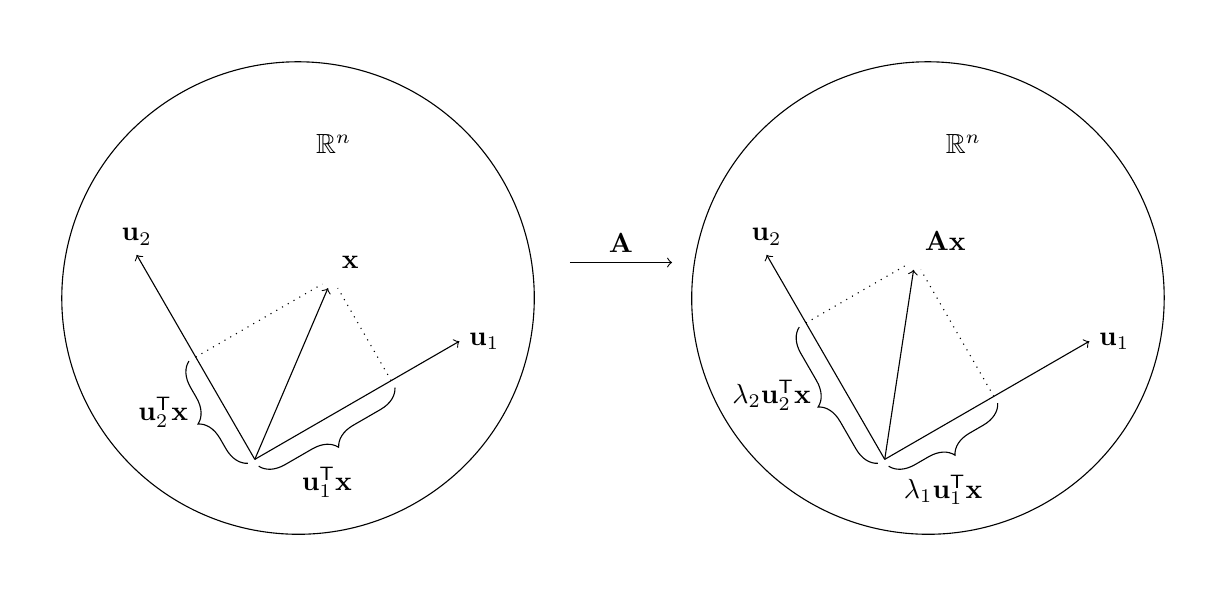
\begin{tikzpicture}
\begin{scope}[rotate = 30]
\node (x) at (2,1.5) {};
  \draw  (1.5,1.5) circle (3cm);
  \draw [->] (0,0) -- (3,0) node[right] {$\mathbf u_1$};
  \draw [->] (0,0) -- (0,3) node[above] {$\mathbf u_2$};
\draw [->] (0,0) -- (x) node[above right] {$\mathbf {x}$};
\draw [dotted] (2,0) -- (x);
\draw [dotted] (0,1.5) -- (x);
\draw [decorate,decoration={brace,amplitude=3mm,mirror},yshift=-1mm] (0,0) -- (2,0) node [midway,yshift=-7mm] { $\mathbf u_1^{\mathsf T} \mathbf x$};
\draw [decorate,decoration={brace,amplitude=3mm},xshift=-1mm] (0,0) -- (0,1.5) node [midway,xshift=-7mm] { $\mathbf u_2^{\mathsf T} \mathbf x$};
\end{scope}
\node at (1,4) {$\mathbb R^n$};

\draw [->] (4,2.5) --  (5.3,2.5)  node [midway,above] {$\mathbf A$};

\begin{scope}[xshift = 8cm]
\begin{scope}[rotate = 30]
\node (x) at (1.6,2) {};
  \draw  (1.5,1.5) circle (3cm);
  \draw [->] (0,0) -- (3,0) node[right] {$\mathbf u_1$};
  \draw [->] (0,0) -- (0,3) node[above] {$\mathbf u_2$};
\draw [->] (0,0) -- (x) node[above right] {$\mathbf {Ax}$};
\draw [dotted] (1.6,0) -- (x);
\draw [dotted] (0,2) -- (x);
\draw [decorate,decoration={brace,amplitude=3mm,mirror},yshift=-1mm] (0,0) -- (1.6,0) node [midway,yshift=-7mm] { $\lambda_1\mathbf u_1^{\mathsf T} \mathbf x$};
\draw [decorate,decoration={brace,amplitude=3mm},xshift=-1mm] (0,0) -- (0,2) node [midway,xshift=-8.5mm] { $\lambda_2\mathbf u_2^{\mathsf T} \mathbf x$};
\end{scope}
\node at (1,4) {$\mathbb R^n$};
\end{scope}
\end{tikzpicture}

\caption{Effect of a real symmetric matrix $\bf A$ of size $n$ on a vector $\bf x$. Only two of the orthogonal eigenvectors are shown. } 
\label{fig:decomp}
\end{figure}

Note that this is a special case of {\em diagonalisation}.  A matrix $\bf A$ is diagonalisable if $\mathbf A = \mathbf {PDP}^{-1}$ (or, equivalently, $\mathbf P^{-1}\mathbf{AP} = \mathbf D$) for some diagonal matrix $\bf D$ and some matrix $\bf P$.  In the case discussed above, where $\bf A$ is real and symmetric, $\bf A$ is diagonalisable with  $\mathbf P = \bf U$ and $\mathbf U^{-1} = \mathbf U^{\mathrm T}$.

%%}%end not in exam

\section{Singular Value Decomposition (SVD)}

Singular Value Decomposition is a method of factorising any ordinary rectangular $m\times n$ matrix.  It is most frequently applied to problems where  $m\ge n$ (more equations than unknowns).

It has  applications in signal processing, pattern recognition, and statistics where it is used for 
 least squares data fitting, regularised inverse problems, finding pseudoinverses and performing principal component analysis (PCA).  The application areas are many and varied but include computational tomography, seismology, weather forecast, image compression, image denoising, genetic analyses and more.
 
It is particularly useful when a given set  of linear equations is singular or very close to 
singular in which case conventional solutions (e.g. by LU decomposition) are either not available or produce senseless results (due to the problems being ill-posed).  In these cases, SVD can diagnose and, in some cases, solve the problem giving an useful numerical answer (though not necessarily the  expected one!).

\subsection{Overview of an SVD}

{\bf SVD} represents an ordinary $m \times n$ matrix $\mathbf{A}$ as 
$\mathbf{A} = \mathbf{UDV}^\mathsf{T}$ where:
\begin{itemize}
\item[$\mathbf{U}$] : an $m \times m$ column-orthogonal matrix; its $m$ columns are the $m$ eigenvectors $\mathbf{u}$ of 
the $m\times m$ matrix $\mathbf{AA}^\mathsf{T}$. The vectors $\{ \mathbf u \}$ are known as the {\em left singular vectors} of $\bf A$.
\item[$\mathbf{V}$] : an $n \times n$ orthogonal matrix; its $n$ columns are the eigenvectors $\mathbf{v}$ of 
the $n\times n$ matrix $\mathbf{A}^\mathsf{T}\mathbf{A}$ . The vectors $\{ \mathbf v \}$ are known as the {\em right singular vectors} of $\bf A$.

\item[$\mathbf{D}$]  : an $m \times n$ matrix whose only non-zero elements are the first $r$ entries on the diagonal where $r$ is the rank of $\bf A$ and  $d_{kk} = \sigma_k = \sqrt \lambda_k$ where $\lambda_k$ is the eigenvalue associated with $\mathbf v_k$.
\end{itemize}
The {\em singular values}, $\sigma_k$ are ordered so that $\sigma_1\ge\sigma_2\ge\ldots\ge\sigma_r > 0$.

Since $\mathbf{A} = \mathbf{UDV}^\mathsf{T}$, we can write
\begin{eqnarray}
\label{eqn:svd} \mathbf{A} & = &\sum_{k = 1}^r \sigma_k \mathbf u_k \mathbf v_k^T \\
\nonumber & = &\sigma_1\mathbf{u}_1\mathbf{v}_1^\mathsf{T}+ 
\sigma_2\mathbf{u}_2\mathbf{v}_2^\mathsf{T }+ \ldots + \sigma_r\mathbf{u}_r\mathbf{v}_r^\mathsf{T}.
\end{eqnarray}
This representation suggests the approximation of $\bf A$ by the truncated series, 
\[
 \mathbf{\widehat A_{\rho}}  = \sum_{k = 1}^{\rho} \sigma_k \mathbf u_k \mathbf v_k^T \mbox{ for } \rho < r.
\]

Notice that when $m > n$ (that is, the problem is over-determined), there are at most $n$ non-zero singular values.  In this case, we can truncate the matrix  $\bf U$ to be $m\times n$ and the matrix $\mathbf D$ to be a $n \times n$ diagonal matrix.  This leaves the sum in Equation \ref{eqn:svd} unaltered as the rows or columns that are removed contribute nothing to that sum. In the following example, we employ this strategy.

{\bf Example}: Find the SVD of the matrix $\bf A$ where 
\[ \mathbf{A}=\left[\begin{array}{rr}0&1\\1&1\\1&0\end{array}\right]
\]
{\bf Solution}:  First find the eigenvectors and eigenvalues of $\mathbf{A}\mathbf{A}^\mathsf{T}$ and $\mathbf{A}^\mathsf{T}\mathbf{A}$.  Since $\bf A$ is $3 \times 2$, we need only find the top two eigenvalues and eigenvectors of each of these matrices.  

\[ \mathbf{A}^\mathsf{T}\mathbf{A}=\left[\begin{array}{rrr}0&1&1\\1&1&0\end{array}\right]
\left[\begin{array}{rr}0&1\\1&1\\1&0\end{array}\right] = \left[\begin{array}{rr}2&1\\1&2\end{array}\right] 
\]
which  has eigenvalues $\lambda_1 = 3$ and $\lambda_2 = 1$.  The associated eigenvectors are, respectively, 
\[ \mathbf{v}_1=\frac{1}{\sqrt{2}}\left[\begin{array}{r}1\\ 1\end{array}\right] \mbox{ and } \mathbf{v}_2=\frac{1}{\sqrt{2}}\left[\begin{array}{r}-1\\ 1\end{array}\right].
\]
Notice that the eigenvectors have been normalised.

Similarly, 
\[ 
\mathbf{A}\mathbf{A}^\mathsf{T}=\left[\begin{array}{rr}0&1\\1&1\\1&0\end{array}\right]
\left[\begin{array}{rrr}0&1&1\\1&1&0\end{array}\right]
=\left[\begin{array}{rrr}1&1&0\\1&2&1\\ 0&1&1\end{array}\right]
\]
The top two eigenvalues are $\mu_1 = 3$ and $\mu_2  = 1$.  Notice that these are the same as the top two eigenvalues of $\mathbf{A}^\mathsf{T}\mathbf{A}$.  The associated eigenvectors are 
\[ \mathbf{u}_1=\frac{1}{\sqrt{6}}\left[\begin{array}{r}1\\ 2\\ 1\end{array}\right] \mbox{ and } 
\mathbf{u}_2=\frac{1}{\sqrt{2}}\left[\begin{array}{r}1\\ 0\\ -1\end{array}\right].
\]
The singular values are given by $\sigma_i = \sqrt \lambda_i$, so $\sigma_1 = \sqrt 3$ and $\sigma_2 = 1$.

We can thus write $\bf A$ as 
\[
\begin{array}{l}
\mathbf{A} = \left[\begin{array}{rr}0&1\\1&1\\1&0\end{array}\right] =
\underbrace{\left[\mathbf{u}_1\;\mathbf{u}_2\right]}_{\mathbf{U}}
\underbrace{\mathrm{diag}(\sigma_1,\sigma_2)}_{\mathbf{D}}
\underbrace{\left[\begin{array}{c}\mathbf{v}_1^\mathsf{T}\\\mathbf{v}_2^\mathsf{T}\end{array}\right]}_{\mathbf{V}^\mathsf{T}}\\
\hspace*{4mm}= 
\underbrace{\left[\begin{array}{rr}1/\sqrt{6}& 1/\sqrt{2}\\
                                                           2/\sqrt{6} & 0                          \\
                                                           1/\sqrt{6} & -1/\sqrt{2}\end{array}\right]}_{\mathbf{U}}
\underbrace{\left[\begin{array}{rr}\sqrt{3}& 0 \\
                                                            0 & 1 \end{array}\right]}_{\mathbf{D}}
\underbrace{\left[\begin{array}{rr}1/\sqrt{2} & 1/\sqrt{2}\\ -1/\sqrt{2} & 1/\sqrt{2}\end{array}\right].}_{\mathbf{V}^\mathsf{T}}
\end{array}
\]
The matrix approximation $\widehat {\mathbf A}_1$ is calculated as follows:
\[
\begin{array}{lll}
\widehat{\mathbf{A}}_1 & = & \sigma_1\mathbf{u}_1 \mathbf{v}_1^\mathsf{T}  \\
& = & 
\sqrt{3} \cdot \frac{1}{\sqrt{6}}\left[ \begin{array}{r} 1 \\ 2\\ 1 \end{array} \right]\cdot\frac{1}{\sqrt{2}}
\left[1\;\;1\right] = \frac{1}{2}
\left[\begin{array}{r} 1\\ 2\\ 1\end{array}\right] \left[1\;\;1\right] = \left[\begin{array}{ll}0.5 & 0.5\\ 1 & 1 \\ 0.5 & 0.5\end{array}\right]\\\\
\end{array}
\]
while the approximation can be extended to  $\widehat {\mathbf A}_2 (= \mathbf A)$ by
\[
\begin{array}{lll}
\widehat{\mathbf{A}}_2 & = & \widehat{\mathbf{A}}_1 + \sigma_2\mathbf{u}_2\mathbf{v}_2^\mathsf{T}\\\\
& \equiv & \left[ \begin{array}{ll}0.5 & 0.5\\ 1 & 1 \\ 0.5 & 0.5\end{array} \right] + 
1\cdot\frac{1}{\sqrt{2}}\left[ \begin{array}{r}1\\ 0\\ -1 \end{array}\right]  \frac{1}{\sqrt{2}}\left[ -1\;\;1 \right] \\ \\
&\equiv & \left[ \begin{array}{ll}0.5 & 0.5\\ 1 & 1 \\ 0.5 & 0.5\end{array} \right] + 
\left[ \begin{array}{rr}-0.5 & 0.5\\ 0 & 0 \\ 0.5 & -0.5\end{array} \right]  = 
\underbrace{ \left[ \begin{array}{rr}0 & 1\\ 1 & 1 \\ 1 & 0\end{array} \right].  }_{\mathbf{A}}
\end{array}
\]

%%\notinexam{
\subsection{How does this all work?\footnote{This section is taken, and condensed, from notes  written by Sze Tan for Physics 707: Inverse Problems.   }} \label{sec:svdexplain}

Recall $\bf A$ is $m\times n$ so that $\mathbf A^T \mathbf A$ is $n\times n$ and $\mathbf {AA}^T$ is $m \times m$.  Both of these product  matrices are square and symmetric.

So, by the result we saw earlier,  $\mathbf A^T\mathbf A$ has $n$ real eigenvalues and a set of $n$ orthonormal eigenvectors (similarly for $\mathbf {AA}^T$ which has $m$ of them).

Let $\mathbf v_i$ be the eigenvectors of $\mathbf {AA}^T$ and $\lambda_i$ be the corresponding eigenvectors and order them so that $\lambda_1 \geq \lambda_2 \geq \ldots \geq \lambda_n \geq 0$. (It can be shown that all eigenvales here are $\geq 0$.)

Similarly, let $\mathbf u_i$ be the eigenvectors of $\mathbf A^T\mathbf A$ and $\mu_i$ be the corresponding eigenvectors and order them so that $\mu_1 \geq \mu_2 \geq \ldots \geq \mu_m \geq 0$.

It turns out that the non-zero eigenvalues of $\mathbf{AA}^T$ are exactly the same as the non-zero eigenvalues of $\mathbf A^T\mathbf A$.  Suppose there are $r$ such non-zero eigenvalues, so that $\lambda_{r+1} = \ldots = \lambda_n = 0$ and $\mu_{r+1} = \ldots = \mu_m = 0$.

$r$ is called the {\em rank} of $\bf A$ (and of $\mathbf A^T$). Clearly, $r \leq m$ and $r \leq n$.

Now, for $k = 1,\ldots, r$, it can be shown that we have 
\[
\mathbf {Av}_k = \sigma_k \mathbf u_k \mbox{ and } \mathbf A^T \mathbf u_k = \sigma_k \mathbf v_k
\]
where $\sigma_k = \sqrt \lambda_k = \sqrt \mu_k$.  And, also that, for $k > r$,
\[
\mathbf {Av}_k = 0 \mbox{ and } \mathbf A^T \mathbf u_k =0.
\]
The equations $\mathbf {Av}_k = \sigma_k \mathbf u_k$ for  $k \leq r$ together with $\mathbf {Av}_k = 0$ for $k >r$ tell us how $\bf A$ acts on the orthonormal set of vectors $\{ \mathbf v_k \}$.  Since this set is  a basis for $\mathbb R^n$, the equations give a complete description of the action of $\bf A$, so that we can write 
\begin{equation} \mathbf A = \sum_{k = 1}^r \sigma_k \mathbf u_k \mathbf v_k ^{\mathrm T}. \label{eqn:svd2}
\end{equation}
A similar argument shows that 
\[ \mathbf A ^{\mathrm T}= \sum_{k = 1}^r \sigma_k \mathbf v_k \mathbf u_k ^{\mathrm T}. \]

The orthonormal vectors $\{ \mathbf v_k \}$ are known as the {\em right singular vectors}, the vectors $\{ \mathbf u_k \}$ are known as the {\em left singular vectors}, and the scalars $\{ \sigma_k \}$ are called the {\em singular values} of the matrix $\mathbf A$.

The singular value decomposition allows us to understand the action of $\mathbf A$ on a vector $\mathbf x$ as 
\[ \mathbf {Ax} = \sum_{k = 1}^r \mathbf u_k \sigma_k ( \mathbf v_k ^{\mathrm T} \mathbf x). 
\]
 which can be interpreted as having  three stages:
\begin{enumerate}
\item It resolves the input vector along each of the right singular vectors $\mathbf v_k$, the component of the input
vector along the $k$th singular vector being given by $\mathbf v_k^T \mathbf x$,
\item The amount along the $k$th direction is multiplied by the singular value $\sigma_k$,
\item The product tells us how much of the $k$th left singular vector $\mathbf u_k$ is present in the product $\mathbf {Ax}$.
\end{enumerate}
This is illustrated in Figure \ref{fig:decomp2}.


\begin{figure}[hbtp]
\centering
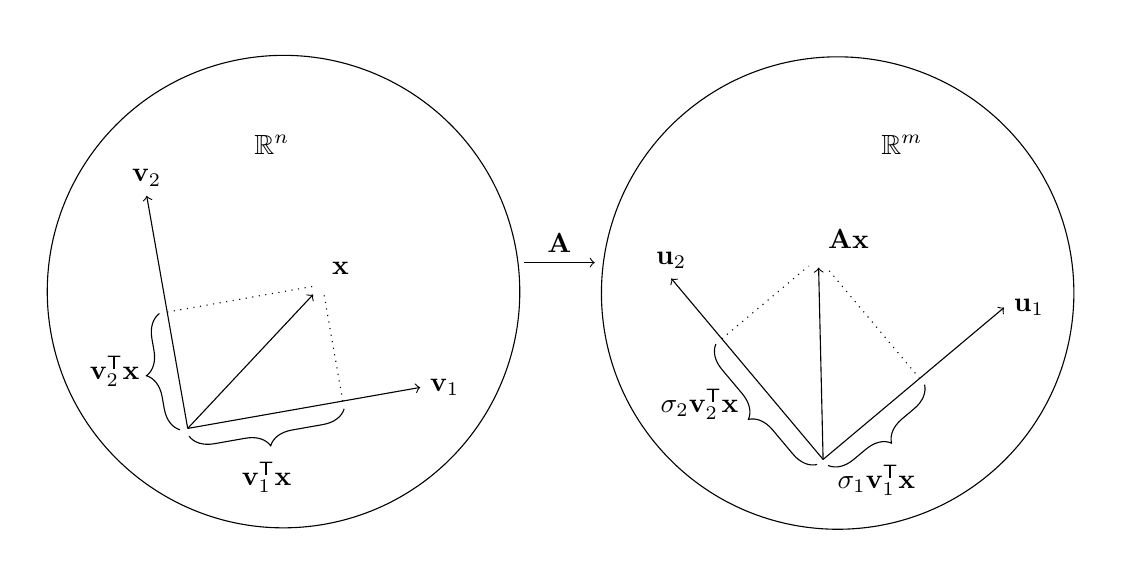
\begin{tikzpicture}
\begin{scope}[rotate = 10,yshift = 4mm]
\node (x) at (2,1.5) {};
  \draw  (1.5,1.5) circle (3cm);
  \draw [->] (0,0) -- (3,0) node[right] {$\mathbf v_1$};
  \draw [->] (0,0) -- (0,3) node[above] {$\mathbf v_2$};
\draw [->] (0,0) -- (x) node[above right] {$\mathbf {x}$};
\draw [dotted] (2,0) -- (x);
\draw [dotted] (0,1.5) -- (x);
\draw [decorate,decoration={brace,amplitude=3mm,mirror},yshift=-1mm] (0,0) -- (2,0) node [midway,yshift=-7mm] { $\mathbf v_1^{\mathsf T} \mathbf x$};
\draw [decorate,decoration={brace,amplitude=3mm},xshift=-1mm] (0,0) -- (0,1.5) node [midway,xshift=-7mm] { $\mathbf v_2^{\mathsf T} \mathbf x$};
\end{scope}
\node at (1,4) {$\mathbb R^n$};

\draw [->] (4.2,2.5) --  (5.1,2.5)  node [midway,above] {$\mathbf A$};

\begin{scope}[xshift = 8cm]
\begin{scope}[rotate = 40]
\node (x) at (1.6,2) {};
  \draw  (1.5,1.5) circle (3cm);
  \draw [->] (0,0) -- (3,0) node[right] {$\mathbf u_1$};
  \draw [->] (0,0) -- (0,3) node[above] {$\mathbf u_2$};
\draw [->] (0,0) -- (x) node[above right] {$\mathbf {Ax}$};
\draw [dotted] (1.6,0) -- (x);
\draw [dotted] (0,2) -- (x);
\draw [decorate,decoration={brace,amplitude=3mm,mirror},yshift=-1mm] (0,0) -- (1.6,0) node [midway,yshift=-7mm] { $\sigma_1\mathbf v_1^{\mathsf T} \mathbf x$};
\draw [decorate,decoration={brace,amplitude=3mm},xshift=-1mm] (0,0) -- (0,2) node [midway,xshift=-8.5mm] { $\sigma_2\mathbf v_2^{\mathsf T} \mathbf x$};
\end{scope}
\node at (1,4) {$\mathbb R^m$};
\end{scope}
\end{tikzpicture}
%\includegraphics[width=12cm]{figures/MatrixDecomp2.pdf}
\caption{Effect of a rectangular  matrix $\bf A$ of size $m\times n$ on a vector $\bf x$. Only two of the orthogonal eigenvectors are shown. }
\label{fig:decomp2}
\end{figure}
%%} %end not in exam


\subsection{Structure of SVD}

In the overdetermined case, in which $m > n$, so that we have more equations than unknowns,  we have the following structure:

\tikz[scale=1.5]{ \small 
\fill[pink] (0,-0.5) -- (0,0.25) -- (0.5,0.25) -- (0.5,-0.5); 
\draw[blue] (0,-0.5) -- (0,0.25) -- (0.5,0.25) -- (0.5,-0.5) -- cycle; 
\node at (0.25,0) {$\mathbf{A}$};
\node at (0.7,0) {$=$};
\fill[pink] (0.9,-0.5) -- (0.9,0.25) -- (1.4,0.25) -- (1.4,-0.5); 
\draw[blue] (0.9,-0.5) -- (0.9,0.25) -- (1.4,0.25) -- (1.4,-0.5) -- cycle; 
\node at (1.15,0) {$\mathbf{U}$};
\fill[pink] (1.5,-0.25) -- (1.5,0.25) -- (2,0.25) -- (2,-0.25); 
\draw[blue] (1.5,-0.25) -- (1.5,0.25) -- (2,0.25) -- (2,-0.25) -- cycle; 
\node at (1.75,0) {$\mathbf{D}$};
\fill[pink] (2.1,-0.25) -- (2.1,0.25) -- (2.6,0.25) -- (2.6,-0.25); 
\draw[blue] (2.1,-0.25) -- (2.1,0.25) -- (2.6,0.25) -- (2.6,-0.25) -- cycle; 
\node at (2.35,0) {$\mathbf{V}^{\mathsf{T}}$};
}

In the underdetermined case, in which $m < n$, so that we have fewer equations than unknowns,  we have the following structure:

\tikz[scale=1.5]{ \small 
\fill[pink] (0,0) -- (0,0.25) -- (0.5,0.25) -- (0.5,0); 
\draw[blue] (0,0) -- (0,0.25) -- (0.5,0.25) -- (0.5,0) -- cycle; 
\node at (0.25,0.12) {$\mathbf{A}$};
\node at (0.7,0.12) {$=$};
\fill[pink] (0.9,0) -- (0.9,0.25) -- (1.4,0.25) -- (1.4,0); 
\draw[blue] (0.9,0) -- (0.9,0.25) -- (1.4,0.25) -- (1.4,0) -- cycle; 
\node at (1.15,0.12) {$\mathbf{U}$};
\fill[pink] (1.5,-0.25) -- (1.5,0.25) -- (2,0.25) -- (2,-0.25); 
\draw[blue] (1.5,-0.25) -- (1.5,0.25) -- (2,0.25) -- (2,-0.25) -- cycle; 
\node at (1.75,0.12) {$\mathbf{D}$};
\fill[pink] (2.1,-0.25) -- (2.1,0.25) -- (2.6,0.25) -- (2.6,-0.25); 
\draw[blue] (2.1,-0.25) -- (2.1,0.25) -- (2.6,0.25) -- (2.6,-0.25) -- cycle; 
\node at (2.35,0.12) {$\mathbf{V}^{\mathsf{T}}$};
}


Note that, in the overdetermined  case,  we truncate $\mathbf U$ and $\mathbf D$ since there are at most $r \leq n < m$ non-zero singular values of $\mathbf A$ we can omit the $\mathbf u_i$ that contribute nothing to matrix product.


The matrix $\mathbf V$ is orthonormal, so $\mathbf {VV}^T = \mathbf V^T\mathbf V = \mathbf I_n$.  $\mathbf U$ is orthonormal when $m \geq n$, but if $m < n$, the singular values $\sigma_j = 0$ for $j = m+1,\ldots, n$ and the corresponding columns of $\mathbf U$ are also 0 so that $\mathbf{UU}^T = \mathrm{diag}(1,\ldots,1,0,\ldots,0)$ where only the first $m$ elements of the diagonal are 1 and the elements from $m+1$ to $n$ are zero.

Note that the SVD of matrix $\mathbf A$ is only unique up to permutations of the columns/rows.  For this reason, we insist that the singular values and corresponding singular vectors are arranged so that the singular values are in descending order $\sigma_1 \geq \sigma_2 \geq \ldots$.  Even then, some of the $\sigma_i$'s may have the same value so columns of $\mathbf U$ and $\mathbf V$ could be permuted.  Aside from these possible permuations, the representation is unique.  Be aware when calculating the SVD with various software that the you may need to enforce this canonical representation.


\subsection{Condition number of a matrix}

The concept of a condition number was introduced in  Section \ref{sec:why}.  This concept can be applied to a matrices and is useful, for example, when considering solutions to the equation $\mathbf {Ax} = \mathbf b$.  Solutions to this equation will change greatly with  small changes in $\mathbf b$ when $\mathbf A$ has a large condition number, while the small changes in  $\mathbf b$ will lead to only small changes in the solution when the matrix has a small condition number.  We can define the condition number of a matrix as the maximum of the  ratio of the relative error in $\mathbf x$ divided by the relative error in $\mathbf b$, where the maximum is taken over all possible $\mathbf x$ and $\mathbf b$.

To give a full description of how to derive the condition number of $\mathbf A$, we would have to introduce matrix norms which we do not have time to do here.  Instead, we simply present the result here that the condition number of $\mathbf A$ can be defined as the ratio of the largest to the smallest non-zero singular values:
\[ cond(\mathbf A) = \frac{\sigma_{\max}}{\sigma_{\min}}. \]
If the smallest singular value of $\mathbf A$ is 0,  $\mathbf A$ is singular (has no inverse) but the condition number of $\mathbf A$ is still defined.



The condition number of $\mathbf A$ is considered to be large, and the matrix is {\em ill-conditioned},  if roughly $\log(cond(\mathbf A)) \geq k $ where $k$ is the number of digits of precision in the matrix entries.

{\bf Example}: Find the condition number of the matrix $\mathbf A = \left[\begin{array}{ll}2 & -3\\1&-1\end{array}\right]$

{\bf Solution}: Using a matrix algebra package, find the singular values of $\mathbf A$ to be $3.864$ and $ 0.259$, so $cond(\mathbf A) = \frac {3.864}{0.259} \approx 14.9$.  \sqend

{\bf Example}: The singular values of the matrix  $\mathbf A = \left[\begin{array}{ll} 1.2969 & 0.8648 \\ 0.2161 & 0.1441 \end{array}\right]$ are approximately $1.58$ and $6.33\times 10^{-9}$ so the condition number is about $2.5\times 10^8$.  This very large condition number means that $\mathbf A$ is an  ill-conditioned matrix.

Ill-conditioning  means that standard approaches to solving linear  systems can be very unstable.  For example, consider the  linear system $\mathbf{Ax} = \mathbf b$ where $\mathbf b = \left[\begin{array}{r} 0.8642 \\ 0.1140 \end{array}\right]$.  This has the exact solution $\mathbf x = \left[\begin{array}{r} 2 \\ -2 \end{array}\right]$. 

But standard matrix software ({\tt linsolve} in Matlab), gives the solution as $\left[\begin{array}{r} 2.59  \\ -3.89  \end{array}\right]\times 10^6$ which is radically wrong!

It also means that if some number in the system is measured slightly differently, the results we get can change enormously.  For example, if  the measurement vector $\mathbf b$ is just slightly different, say $\mathbf b = \left[\begin{array}{r} 0.86419999 \\ 0.11400001 \end{array}\right]$, then the exact solution is now close to $\mathbf x = \left[\begin{array}{r} 0.9911 \\ -0.4870 \end{array}\right]$ which represents an enormous change in the solution relative to the small change in the original system. \sqend

%%\notinexam{




%\subsection{Applications of SVD}

We'll see in a later section on pseudo-inverses how the SVD can be used to solve the linear system $\mathbf{Ax} = \mathbf b$.


\subsubsection{Image compression}

See slides and assignment 1.

\subsubsection{Gene expression}

Abstract from Alter et al, 2000, {\em Singular value decomposition for genome-wide expression data processing and modeling},  \url{http://www.pnas.org/content/97/18/10101.full}: We describe the use of singular value decomposition in transforming genome-wide expression data from genes $\times$ arrays space to reduced diagonalized ``eigengenes'' $\times$ `eigenarrays'' space, where the eigengenes (or eigenarrays) are unique orthonormal superpositions of the genes (or arrays). Normalizing the data by filtering out the eigengenes (and eigenarrays) that are inferred to represent noise or experimental artifacts enables meaningful comparison of the expression of different genes across different arrays in different experiments. Sorting the data according to the eigengenes and eigenarrays gives a global picture of the dynamics of gene expression, in which individual genes and arrays appear to be classified into groups of similar regulation and function, or similar cellular state and biological phenotype, respectively. After normalization and sorting, the significant eigengenes and eigenarrays can be associated with observed genome-wide effects of regulators, or with measured samples, in which these regulators are overactive or underactive, respectively. 

%
%
%
% \newpage
%%}%end not in exam


\subsection{Principal Components Analysis (PCA)}



PCA is a common technique for identifying patterns in high-dimensional data.  It  transforms   the original correlated measurements into uncorrelated measurements.
 One of the main uses of PCA is as a dimension reduction tool, in which only the directions in which the data varies the most are considered.  This can lead to enormous simplifications of the data and provide insights for a wide variety of data.   PCA is alternatively known as  the Karhunen-Lo\'eve transform (KLT), the Hotelling transform or proper orthogonal decomposition (POD)
 
 These new coordinate axes (along which the data varies the most) are are known as {\em principal components} and are, by construction, orthogonal.

 A useful visualisation tool to aid your understanding of PCA is at \href{http://setosa.io/ev/principal-component-analysis/}{http://setosa.io/ev/principal-component-analysis/}.


Suppose we have a  $m \times n$ matrix of measurement data $A$.  For example, $n$ trials where $m$ properties were measured in each trial.  Then, if $\mathbf a_i$ are the measurements from the $i$th trial,  
\[
\mathbf{A} = \left[\begin{array}{cccc}\mathbf{a}_1 & \mathbf{a}_2 & \ldots & \mathbf{a}_n \end{array}\right]
= \left[\begin{array}{cccc}
a_{11} & a_{12} & \ldots & a_{1n}\\
a_{21} & a_{22} & \ldots & a_{2n}\\
\vdots  &  \vdots & \ddots & \vdots \\
a_{m1} & a_{m2} & \ldots & a_{mn}\\
 \end{array}\right].
\]
For example, $\bf A$ could be $n = 100$ observations of the position of an object measured in $m = 3$ dimensions.

%In the following, assume that the columns of $\mathbf A^{\mathsf T}$ have been centred, so that the mean of each column is 0 (the columns of $\mathbf A^T$ are just the rows of $\mathbf A$ so correspond to each dimension of the measurements). If this is not already the case, it can be achieved by subtracting the mean of each column of $\mathbf A^T$ from each element of that column. That is, set element  \[a_{ij} = a_{ij}- \sum_{j = 1}^n a_{ij}/n\] to centre the rows of $\mathbf A$ and, therefore, the columns of $\mathbf A^T$.  This is a critical assumption and allows us to concentrate on the variance. 
In the following, assume that the rows of $\mathbf A$ have been centred, so that the mean of each row is 0 (each rows of $\mathbf A$  corresponds to a dimension in the original data). If this is not already the case, it can be achieved by subtracting the mean of each row of $\mathbf A$ from each element of that row. That is, set element  \[a_{ij} = a_{ij}- \sum_{j = 1}^n a_{ij}/n\] to centre the rows of $\mathbf A$.  This is a critical assumption and allows us to concentrate on the variance. 

Each observation $\bf A$ is just the $m$-vector $\mathbf a_i$. The idea of PCA is to chose a new basis $\mathbf u_1, \ldots, \mathbf u_k$ to express the data points (the $\mathbf a_i$'s) so that the variance of the measurements  is greatest in the direction of $\mathbf u_1$, the next greatest variance is in the direction of $\mathbf u_2$ and so on, down to $\mathbf u_k$.  Ideally, $k < m$.

Define the {\em covariance matrix} of $\mathbf A$ by 
\[\mathbf \Sigma = \frac 1 {n-1} \mathbf {AA}^T. \] %\approx \frac 1 {n} \mathbf {AA^T} .\]
Then $\mathbf \Sigma$ is an $m \times m$ matrix where the diagonal terms of $\mathbf \Sigma $ are the variance of the $i$th dimension of the measurement, while the off-diagonal terms of $\mathbf \Sigma $ are the covariances between different measurements.  

It turns out that the best basis to choose are the $k$ eigenvectors of $\mathbf \Sigma$  corresponding its $k$ largest eigenvalues.  These are known as the {\em principal components} of $\mathbf A$.  Call them $\mathbf u_1, \ldots, \mathbf u_k$ and form the matrix 
\[
\mathbf U_k = [\mathbf u_1, \ldots, \mathbf u_k]
\]
From results we have seen earlier about symmetric matrices, this an orthogonal matrix.  We include the subscript $k$ as we may decide to truncate this matrix by including only the eigenvectors corresponding to the largest eigenvalues.  That is, if $\mathbf \Sigma$ has $K$ eigenvectors and associated eigenvalues, and the largest $k$ eigenvalues are substantially larger than the remaining $K-k$, it is reasonable to form $ \mathbf U_k$ containing only the most significant $k$ eigenvectors.



We can now represent  the original measurements, $\mathbf A$, in this this new co-ordinate system.   The amount of measurement vector $\mathbf a_i$ in direction $\mathbf u_j$ is given by $\mathbf u_j^\top  \mathbf a_i$:  this is the  $j$th coordinate of $\mathbf a_i$ in this new coordinate system.  So if we consider just the two dimension space defined by the top two principal components,  $\mathbf a_i$ has coordinates  \[ \mathbf{U}_2^\mathsf{T} \mathbf a_i  = 
\left[\begin{array}{c}
\mathbf{u}_1^\mathsf{T}\\ \mathbf{u}_2^\mathsf{T} 
\end{array}\right] \mathbf a_i 
= 
\left[\begin{array}{c}
\mathbf{u}_1^\mathsf{T}\mathbf a_i \\ \mathbf{u}_2^\mathsf{T} \mathbf a_i
\end{array}\right]. \]

We usually consider this space independently of how it relates to the original $m$-dimensional space but we can consider it as embedded in the original  space.
%and he original points projected onto that embedded lower dimensional space.  
To find the coordinates of a point in this embedded space, define the projection matrix, $\mathbf P_k$  by
\[
\mathbf{P}_k = \mathbf{U}_k\mathbf{U}_k^\mathsf{T} = 
\left[\begin{array}{cccc}
\mathbf{u}_1 & \mathbf{u}_2 & \ldots & \mathbf{u}_k
\end{array}\right]
\left[\begin{array}{c}
\mathbf{u}_1^\mathsf{T}\\ \mathbf{u}_2^\mathsf{T}\\ \vdots \\ \mathbf{u}_k^\mathsf{T}
\end{array}\right]
\]
so that each measurement vector $\mathbf a_i$ is projected via $\mathbf P_k \mathbf a_i$.  

One interpretation of PCA is that the projection $\mathbf{P}_k$ is chosen to minimise the projection error
$\sum_{j=1}^n\|\mathbf{a}_j-\mathbf{P}_k\mathbf{a}_j\|^2$


{\bf Example:} Find the principal components of the data matrix $\mathbf A$ where 
\[ \mathbf A= \left[ 
\begin{array}{rrrrrr}
  -4   & 3  & -5  & 18 &   6  & -5 \\
    2  &  6  & -2  & 10   & 1 &  -1 \\ 
    7 &  11  &  3 &   6  &  9 &   3 \\
\end{array} \right].
\]
Find the amount of the first principal component in the first measurement vector of $\mathbf A$ (that is, the first column), and calculate the projection matrix for projecting  $\mathbf A$ onto the first two principal components.


{\bf Solution:} First, centre the rows of $\mathbf A$ so that each row has mean zero.  Call this centred matrix $\mathbf B$.
\[ \mathbf B= \left[ 
\begin{array}{rrrrrr}
 -6.1667 & 0.8333 & -7.1667 & 15.8333  & 3.8333 & -7.1667 \\
 -0.6667 & 3.3333 & -4.6667 & 7.3333 & -1.6667 & -3.6667\\
  0.5 & 4.5 & -3.5 & -0.5 & 2.5 & -3.5\\
\end{array} \right].
\]
Now form the covariance matrix for the centred data matrix,  $\mathbf{\Sigma}  = \frac 1 n \mathbf B \mathbf B^{\mathsf T}$:
\[ \mathbf \Sigma = \frac 1 5 \left[ 
\begin{array}{rrr}
 406.8333 &176.3333   &  52.5\\
 176.3333 & 103.3333 &  36.0\\
  52.5000  & 36.0000 & 51.5\\
\end{array} \right].
\]
This matrix has eigenvalues $99.31, \;  9.46$ and  $ 3.561$ corresponding to eigenvectors 
\[ [\mathbf u_1, \mathbf u_2, \mathbf u_3] =  \left[ 
\begin{array}{rrr}
 0.8987 & 0.2829 & 0.3352 \\ 
 0.4158 & -0.3062 & -0.8564 \\ 
 0.1396 & -0.9090 & 0.3928  
 \end{array} \right] = \mathbf U.
\]
These eigenvectors are the principal components of $\mathbf A$ (and of $\mathbf B$).  

The amount  of the first principal component in $\mathbf a_1$ is $$\mathbf u_1^\top \mathbf a_1 =   
[0.8987, 0.4158, 0.1396] \left[\begin{array}{r}
-4 \\ 2\\ 7 \end{array} \right] = -1.756.
$$

To project   $\mathbf A$ into the  coordinate system defined by the first two principal components, form the projection matrix, \[\mathbf P_2  =  \mathbf{U}_2\mathbf{U}_2^\mathsf{T} = \left[ 
\begin{array}{rrr}
 0.8987 & 0.2829  \\
 0.4158 &-0.3062  \\
 0.1396 & -0.9090 \\
\end{array} \right] \left[ 
\begin{array}{rrr}
 0.8987 & 0.4158 &  0.1396 \\ 
 0.2829  & -0.3062 & -0.9090 \\
\end{array} \right]  =
\left[ 
\begin{array}{rrr}
  0.8877 &0.2870 &-0.1316 \\
  0.2870& 0.2666 & 0.3364\\
 -0.1316& 0.3368 & 0.8457\\
\end{array} \right] 
\]


%%\notinexam{
\subsection{Examples}
\label{sec:svdexamples}
See associated slides for population structure in Europe (Novembre et al, Nature 2008, \url{http://www.nature.com/nature/journal/v456/n7218/full/nature07331.html} )and Eigenfaces.

The ``eigenfaces'' example in the slides was developed by Matthew Turk and Alex Pentland (Journal of Cognitive Neuroscience, 1991, v3 (1)). The following quote is from their abstract:
\begin{quote}
We have developed a near-real-time computer system that can locate and track a subject's head, and then recognize the person by comparing characteristics of the face to those of known individuals. ... The system functions by projecting face images onto a feature space that spans the significant variations among known face images. The significant features are known as "eigenfaces," because they are the eigenvectors (principal components) of the set of faces; they do not necessarily correspond to features such as eyes, ears, and noses. The projection operation characterizes an individual face by a weighted sum of the eigenface features, and so to recognize a particular face it is necessary only to compare these weights to those of known individuals. Some particular advantages of our approach are that it provides for the ability to learn and later recognize new faces in an unsupervised manner, and that it is easy to implement using a neural network architecture.
\end{quote}
% 
%%}%end not in exam

\subsection{What is connection between PCA and SVD?}

Given $\mathbf A$  such that the rows of $\mathbf A$ have zero mean, define $\mathbf Y = \frac 1 {\sqrt {n-1}} \mathbf A^T$ (which has  columns with zero mean).  Then $\mathbf Y^T\mathbf Y = \mathbf \Sigma$, the covariance of $\mathbf A$.  We have seen  that the principal components of $\mathbf A$ are the eigenvectors of $\mathbf \Sigma$. 

Now, if we calculate the SVD of $\mathbf Y$ to get $\mathbf Y = \mathbf{UDV}^T$, the columns of $\mathbf V$ are the eigenvectors of $\mathbf Y^T \mathbf Y = \mathbf \Sigma$. Therefore, the columns of $\mathbf V$ are the principal components of $\mathbf A$.
 

\subsection{Problems with SVD and PCA}

As we have seen, SVD and PCA are powerful analysis tools and SVD is a very stable procedure.  They do not, however, come free of cost.  

The time complexity of SVD is $O(m^2n + n^3)$ to calculate all of $\mathbf U, \mathbf V$ and $\mathbf D$ (where, typically, $m \gg n$) while faster algorithms are available when some elements of the SVD are not required.

However, the matrices  $\mathbf{U}$ and $\mathbf{V}$ are not at all {\em sparse}, where we say a matrix is sparse when it mainly consists of zeros. Spareness is a commonly assumed property in large systems as it reflects the observation that most effects are local and do not influence all parameters in the system ---  a large world  with small neighbourhoods.  Sparse matrices are typically computationally efficient to work with and store. 

A second potential set-back is that SVD and PCA only work with data that can be (coherently) expressed as a two dimensional array (that is, a matrix).  When data naturally has 3 or 4 dimensions arrays ({\em tensors}), as is common in many engineering applications, there is no perfect analogue to SVD or PCA or even eigenvectors.  

Finally, when using PCA for data analysis,  you should be aware of the strong assumptions being made.  In particular, dependencies in the data are assumed to be linear, which may not be the case.  PCA and SVD will always give an answer but it is up to the user to interpret whether or not it is a valid answer to any question they are interested in.
   

\section{Least squares} \label{sec:leastsquares}


\begin{figure}[h]
\includegraphics[width=6cm]{figures/kidiq}
\includegraphics[width=6cm]{figures/kidiqlm}
\caption{Left: Relationship between cognitive test scores for 3-4 year old children and mother's IQ score. Right: The same data with a least squares best fit line added. Discussed in Gelman and Hill, 2007, Cambridge University Press, data at \href{http://www.stat.columbia.edu/~gelman/arm/examples/child.iq/kidiq.dta}{http://www.stat.columbia.edu/~gelman/arm/examples/child.iq/kidiq.dta}}
\label{fig:leastsq}
\end{figure}

You are probably familiar with the basic idea of least squares: we have a set of measurements and we want to fit a model to them.  But no sufficiently simple model exactly fits all of the points at the same time. So how choose the model that is most satisfactory?  The answer often given is that we chose the model that satisfies the {\em least squares} criterion:  that is, the model for which the sum of the squares of differences between the predictions from the model and the actual observations is minimised.  

For example, in Figure  \ref{fig:leastsq}, we might want to fit a linear model to the relationship between a mother's IQ score and her young child's score in a cognitive test. This should be familiar to you as the linear regression problem in statistics.

This problem arises when we have an {\em overdetermined} linear system: recall that 
$\mathbf{Au} = \mathbf{b}$ is overdetermined when  $\mathbf{A}$ is  $m \times n$ matrix with $m > n$:
\[
\left[\begin{array}{cccc}
a_{11} & a_{12} & \ldots & a_{1n} \\
a_{21} & a_{22} & \ldots & a_{2n} \\
\vdots & \vdots & \ddots & \vdots \\
a_{m1} & a_{m2} & \ldots & a_{mn} 
\end{array}\right]\left[\begin{array}{c}u_1 \\ u_2 \\\vdots\\u_n\end{array}\right] =
\left[\begin{array}{c}b_1 \\ b_2 \\\vdots\\b_m\end{array}\right].
\]
In this case, $\mathbf A^{-1}$ does not exist and there is no $\mathbf u$ that solves this problem.  (We ignore the highly unusual cases where a solution does exist.)

The goal, then, is to find the  best solution $\mathbf u^*$ to the problem.  

{{\bf Example 1}: Fitting $m=4$ measurements by a small number $n=2$ of parameters (e.g. linear regression in statistics)}

Want to find the  straight line $b_x = u_1 + u_2x$ where we have observed the points  $b_x$ at $x$.
\[
\begin{array}{l}
\left\{\begin{array}{rcl}
u_1 + u_2 \cdot 0 & = &1\\
u_1 + u_2\cdot 1 & = & 9\\
u_1 + u_2\cdot 2 & = & 9 \\
u_1 + u_2\cdot 4 & = & 21
\end{array}\right. \; {\Leftrightarrow} \\\\
\left\{\left[\begin{array}{cc} 1&0\\1&1\\1&3\\1&4\end{array}\right]\right.
\left[\begin{array}{c}u_1\\ u_2\end{array}\right]=\left[\begin{array}{r}1\\9\\9\\21\end{array}\right]
\end{array}
\]
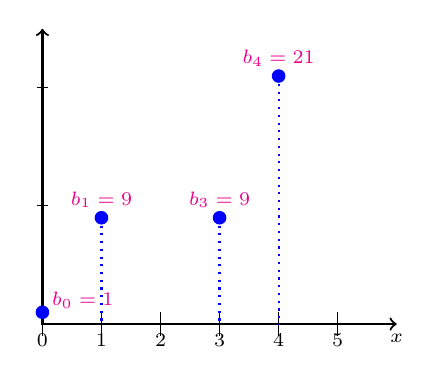
\begin{tikzpicture}[xshift=-4cm,scale=1.5]
\draw[thick,<->] (4,1.5) -- (4,-1) -- (7,-1);
\foreach \x in {4,4.5,...,6.5} \draw (\x,-0.9) -- (\x,-1.1);
\foreach \x in {0,1} \draw (3.95,\x) -- (4.05,\x);
\node[below] at (7,-1) {\scriptsize $x$};
\node[below] at (4,-1) {\scriptsize $0$};
\filldraw[blue] (4,-0.9) circle (1.5pt);
\node[right,magenta] at (4,-0.8) {\scriptsize $b_0=1$};
\node[below] at (4.5,-1) {\scriptsize $1$};
\filldraw[blue] (4.5,-0.1) circle (1.5pt);
\draw[dotted,blue,thick] (4.5,-0.1) -- (4.5,-1);
\node[above,magenta] at (4.5,-0.1) {\scriptsize $b_1=9$};
\node[below] at (5,-1) {\scriptsize $2$};
\node[below] at (5.5,-1) {\scriptsize $3$};
\filldraw[blue] (5.5,-0.1) circle (1.5pt);
\draw[dotted,blue,thick] (5.5,-0.1) -- (5.5,-1);
\node[above,magenta] at (5.5,-0.1) {\scriptsize $b_3=9$};
\node[below] at (6,-1) {\scriptsize $4$};
\filldraw[blue] (6,1.1) circle (1.5pt);
\draw[dotted,blue,thick] (6,1.1) -- (6,-1);
\node[above,magenta] at (6,1.1) {\scriptsize $b_4=21$};
\node[below] at (6.5,-1) {\scriptsize $5$};
\end{tikzpicture}

The above set of equations clearly has no solution as vector $\mathbf{b}$ is not a linear combination of the two column vectors from $\mathbf{A}$: 
\[
\left[\begin{array}{cc} 1&0\\1&1\\1&3\\1&4\end{array}\right]
\left[\begin{array}{c}u_1\\ u_2\end{array}\right]\ne\left[\begin{array}{r}1\\9\\9\\21\end{array}\right]
\]

For example, The line $b = 1 + 8x$ through the first two points is almost certainly not the best line:

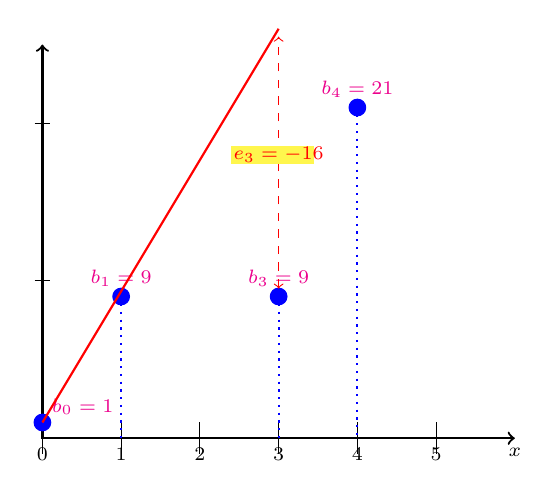
\begin{tikzpicture}[scale=2]
\draw[thick,<->] (0,1.5) -- (0,-1) -- (3,-1);
\foreach \x in {0,0.5,...,2.5} \draw (\x,-0.9) -- (\x,-1.1);
\foreach \x in {0,1} \draw (-0.05,\x) -- (0.05,\x);
\node[below] at (3,-1) {\scriptsize $x$};
\node[below] at (0,-1) {\scriptsize $0$};
\filldraw[blue] (0,-0.9) circle (1.5pt);
\node[right,magenta] at (0,-0.8) {\scriptsize $b_0=1$};
\node[below] at (0.5,-1) {\scriptsize $1$};
\filldraw[blue] (0.5,-0.1) circle (1.5pt);
\draw[dotted,blue,thick] (0.5,-0.1) -- (0.5,-1);
\node[above,magenta] at (0.5,-0.1) {\scriptsize $b_1=9$};
\node[below] at (1,-1) {\scriptsize $2$};
\node[below] at (1.5,-1) {\scriptsize $3$};
\filldraw[blue] (1.5,-0.1) circle (1.5pt);
\draw[dotted,blue,thick] (1.5,-0.1) -- (1.5,-1);
\node[above,magenta] at (1.5,-0.1) {\scriptsize $b_3=9$};
\node[below] at (2,-1) {\scriptsize $4$};
\filldraw[blue] (2,1.1) circle (1.5pt);
\draw[dotted,blue,thick] (2,1.1) -- (2,-1);
\node[above,magenta] at (2,1.1) {\scriptsize $b_4=21$};
\node[below] at (2.5,-1) {\scriptsize $5$};
\draw[red,thick] (0,-0.9) -- (1.5,1.6);
\draw[red,dashed,<->] (1.5,-0.05) -- (1.5,1.55) node[fill,yellow!70] at (1.46,0.8) {~~~~~~~~} node at (1.5,0.8) {\scriptsize $e_3=-16$};
\end{tikzpicture}

But why is this not the best line: look at the {\em error} or {\em residual }, $\mathbf{e}=\mathbf{b}-\mathbf{Au}$.  For the two points the line does not pass through the error is $e_x=b_x-(1+8x)$
is large: $e_3=16$ and $e_4 = 12$.  The {\em Total square error}, $E(\mathbf u) = 0 + 0 + 256 + 144  =400$ .

Notice that the {\em total square error} is given by. 
\[ E(\mathbf u) = \mathbf{e}^{\mathsf{T}}\mathbf{e}\equiv\parallel\mathbf{e}\parallel^2
=(\mathbf{b}-\mathbf{Au})^{\mathsf{T}}(\mathbf{b}-\mathbf{Au})
\]

The Least Squares method  to find the chooses a solution $\mathbf u^*$ that minimises $E(\mathbf u)$.
 
How do we find $\mathbf u^*$?  To find the minimum of $E(\mathbf u)$, we can differentiate with respect to $\mathbf u$, set to 0 and attempt to solve for $\mathbf u$:
\[
\begin{array}{rcl}
 E(\mathbf{u}) &=&(\mathbf{b}-\mathbf{Au})^\mathsf{T}(\mathbf{b}-\mathbf{Au}) \\ \\ 
 &= & \mathbf{b}^\mathsf{T}\mathbf{b} - 2\mathbf{u}^\mathsf{T}\mathbf{A}^\mathsf{T}\mathbf{b}+\mathbf{u}^\mathsf{T} \mathbf{A}^\mathsf{T}\mathbf{A}\mathbf{u}
\end{array}
 \]
 Differentiating and setting to 0:
 \[
 \begin{array}{rrl}
  & \frac{\partial E(\mathbf{u})}{\partial \mathbf{u}} = & 0 \\ \\
\implies  & -2\mathbf{A}^\mathsf{T}\mathbf{b} + 2\mathbf{A}^\mathsf{T}\mathbf{A}\mathbf{u} = & \mathbf{0}\\ \\
\implies  & \mathbf{A}^\mathsf{T}\mathbf{A}\mathbf{u} =& \mathbf{A}^\mathsf{T}\mathbf{b} 
\end{array}
\]
This equation, $\mathbf{A}^\mathsf{T}\mathbf{A}\mathbf{u} = \mathbf{A}^\mathsf{T}\mathbf{b}  $ is called the {\em normal equation}.  

The least squares estimate, $\mathbf{u^*}$, is the solution  to the normal equation.

Notice that $\mathbf A^T \mathbf A$ is square and symmetric.    In some cases it may be possible to directly find the inverse (in particular, when $\mathbf A$ has independent columns, then $\mathbf A^T \mathbf A$ is  positive definite and $\mathbf A^T \mathbf A$ is invertible in which case $\mathbf u^* = ( \mathbf{A}^\mathsf{T}\mathbf{A})^{-1}\mathbf{A}^\mathsf{T}\mathbf{b}$).  In other cases, this approach may be highly unstable, so stable numerical techniques need to be employed.




%%\notinexam{
\subsection{Understanding the Least Squares solution }
\label{sec:leastsqexplain}
{\em This subsection is not examined}.
The main point of this section is to add some geometric and algebraic understanding  to our discussion.  You are not expected to understand all the detail in this section, but do familiarise yourself with the concept and definition of the projection matrix $\mathbf P$ defined below.


The equation $\mathbf{Au} = \mathbf b$ can be seen as  attempting to represent $\mathbf b$   as a linear combination of the $n$ columns of $\mathbf A$.  This is impossible, since the $n$ columns of $\mathbf A$ describe, at most, an $n$-dimensional plane inside the much larger $m$ dimensional space (recall that $n < m$).  Thus $b$ is unlikely to fall on that plane.  The plane is called the {\em column space} of $\mathbf  A$.

\tikz[scale=1.25]{
\draw[fill,yellow!20] (0,0) -- (5,1) -- (6,-1) -- (1,-2) -- cycle;
\draw (0,0) -- (5,1) -- (6,-1) node[left] at (6,-0.7) {\small {\bf column space}} -- (1,-2) -- cycle;
\draw[blue,<->]  (5,0.2) node[above] at (5,0.1) {column $\mathbf{a}_1$} -- (0.8,-0.3) -- (1.2,-1.6) 
node[below] at (1.2,-1.4) {column $\mathbf{a}_n$};
\filldraw (0.8,-0.3) circle (1.5pt); 
\draw[thick] (0.8,-0.3) -- (2,1);
\draw[thick] (0.8,-0.3) -- (2,-1);
\draw[thick,->,dashed] (2,-1) -- (2,0.95) 
node[right] at (1.9,0.2) {\small $\mathbf{e}=\mathbf{b}-\mathbf{Au}^\ast$}
node[right] at (1.9,-0.3) {\scriptsize $\parallel\mathbf{e}\parallel^2 = \parallel\mathbf{b}\parallel^2 - \parallel\mathbf{p}\parallel^2$};
\filldraw[blue] (2,1) circle (1.5pt);
\filldraw[red] (2,-1) circle (1.5pt) node[right] {$\mathbf{p}=\mathbf{Au}^\ast$}; 
\filldraw[yellow!50] (2.2,-2) rectangle (7.5,-1.5);
\draw[thick] (2.2,-2) rectangle (7.5,-1.5); 
\draw (2.2,-1.75) node[right] {\small The best $\mathbf{Au}^\ast$ is the projection $\mathbf{p}$};
}


The best solution, $\mathbf A\mathbf u^* $, is the nearest point to $\mathbf b$ on that plane. Call this point $\mathbf p = \mathbf {Au}^*$.

Now, from a geometric argument, you can see that the error vector $\mathbf e$ is orthogonal (perpendicular) to this plane.  Thus $\mathbf A^T e = 0$.

Notice that  $0 = \mathbf A^T \mathbf e = \mathbf A^T(\mathbf b-\mathbf {Au}^*) = \mathbf A^T\mathbf b - \mathbf A^T\mathbf {Au}^* \implies \mathbf A^T\mathbf b = \mathbf A^T\mathbf{Au}^*$.
This is a geometric derivation of  the normal equation that we earlier saw derived from calculus.  

The point  $\mathbf  p \; (= \mathbf {Au}^*)$ is the projection of $\mathbf b$ onto the column space of $\mathbf A$:
\[
\mathbf{p} = \mathbf{Au}^\ast = 
\underbrace{\left[\mathbf{A}\left(\mathbf{A}^\mathsf{T}\mathbf{A}\right)^{-1}\mathbf{A}^\mathsf{T}\right]}_{\textsf{projection matrix }\mathbf{P}}
\mathbf{b} = \mathbf{Pb},
\]
where we define the {\em Projection matrix}, $\mathbf{P} = \mathbf{A}\left(\mathbf{A}^\mathsf{T}\mathbf{A}\right)^{-1}\mathbf{A}^\mathsf{T}$.  $\mathbf P$ is symmetric and of size $m \times m$ but the rank of $\mathbf P$ is only $n$ (as all the factors of $\mathbf P$ in the definition above have rank $n$).
%%}%end not in exam


\subsection{Computing the Least Squares solution, $\mathbf u^*$ }

We consider three methods for computing the least squares solution to a linear system.  They are Gaussian elimination, QR Decomposition (aka Orthogonalisation) and computation of the pseudo-inverse via SVD.


\subsection{Computing $\mathbf u^*$ via Gaussian elimination}

Given the normal equation $\mathbf A^T\mathbf{Au} = \mathbf A^T\mathbf b$, we may be tempted to find the solution  by Gaussian elimination, where we reduce the the matrix $\mathbf A^T \mathbf A$ to upper triangular form using elementary row operations.

This solution can work but is highly unstable.  To see why it is unstable, consider the condition number of the matrix $\mathbf A^T \mathbf A$.   It can be shown that the condition number of $\mathbf A^T \mathbf A$ is the square of the condition number of $\mathbf A$  (if we take $\sigma_{\min}$ to be the smallest non-zero singular value in the definition of condition number).  So  even if $\mathbf A$ has only moderately widely spread singular values, $\mathbf A^T\mathbf A$  can have a very large condition number and solution by row reduction can be very unstable.




\subsection{Computing $\mathbf u^*$ via orthogonalisation (QR decomposition)}

QR-decompostion presents a much more stable solution to   the normal equation $\mathbf A^\mathrm T\mathbf{Au} = \mathbf A^ \mathrm T\mathbf b$.

The  Orthogonalisation of matrix $\mathbf A$ is given by $\mathbf A = \mathbf {QR}$ where
\begin{itemize}
\item $\mathbf{Q}$ is an $m\times n$ matrix with $n$ orthonormal columns:
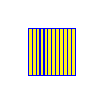
\begin{tikzpicture}
\filldraw[yellow!90] (0,0) -- (0,0.6) -- (0.6,0.6) -- (0.6,0) -- cycle; 
\draw[blue] (0,0) -- (0,0.6) -- (0.6,0.6) --(0.6,0) -- cycle; 
\foreach \x in {0.05,0.1,...,0.6} \draw[blue] (\x,0) -- (\x,0.6);
\end{tikzpicture}.  Construction of $\mathbf Q$ is discussed below.

\item $\mathbf{R }$ is an $n\times n$ upper triangular matrix:
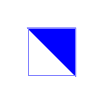
\begin{tikzpicture}
\filldraw[blue] (0.6,0) -- (0,0.6) -- (0.6,0.6) -- cycle; \draw[blue!50] (0,0) -- (0,0.6) -- (0.6,0.6) -- (0.6,0) -- cycle; 
\end{tikzpicture}.  $\mathbf R$ is given by $\mathbf R = \mathbf Q^\mathrm T \mathbf A$.

\end{itemize}


 This factorisation  reduces the normal equation  to a much simpler equation:
\begin{eqnarray*}
\mathbf{A}^\mathsf{T}\mathbf{A}\mathbf{u}&=&\mathbf{A}^\mathsf{T}\mathbf{b}\\
\implies (\mathbf{Q}\mathbf{R})^\mathsf{T}\mathbf{Q}\mathbf{R}\mathbf{u}^\ast &=& (\mathbf{Q}\mathbf{R})^\mathsf{T}\mathbf{b} \\
{\implies}\; \mathbf{R}^\mathsf{T}\mathbf{Q}^\mathsf{T}\mathbf{Q}\mathbf{R}\mathbf{u}^\ast &=&
\mathbf{R}^\mathsf{T}\mathbf{Q}^\mathsf{T}\mathbf{b}
\\
{\implies}\; 
 \mathbf{R}^\mathsf{T} \mathbf{R}\mathbf{u}^\ast &=& \mathbf{R}^\mathsf{T}\mathbf{Q}^\mathsf{T}\mathbf{b} \mbox{ since $\mathbf Q^\mathsf{T}\mathbf Q = \mathbf I $}\\
 {\implies}\; \mathbf{R}\mathbf{u}^\ast  &=& \mathbf{Q}^\mathsf{T}\mathbf{b} \mbox{ multiplying both sides by } (\mathbf{R}^\mathsf{T})^{-1}.
 \end{eqnarray*}
This is easy to solve via back-substitution, since $\mathbf R$ is upper triangular.


\subsubsection{Constructing  the orthogonal matrix $\mathbf Q$ by Gram-Schmidt}

The orthonormal columns of $\mathbf Q$, call them $\mathbf q_1,\ldots, \mathbf q_n$, are obtained iteratively  from the columns $\mathbf{a}_1,\ldots,\mathbf{a}_n$ of $\mathbf{A}$.  The basic idea is that we set $\mathbf q_1$ to be $\mathbf a_1$.  $q_2$ is then set to be $a_2$ and any part of it in the direction of $q_1 (=a_1)$ is subtracted out, so ensure that it is orthogonal to $q_1$.  Similarly, $q_3$ is set to be $a_3$ with any parts in the direction of $q_1$ or $q_2$ are subtracted.  All these vectors are normalised to have magnitude 1 at each step.

This is called the {\em Gram-Schmidt} process and is more formally defined as follows:

\[
\begin{array}{lllll}
\mbox{Set } \mathbf{v}_1&= &  \mathbf{a}_1. &\mbox{ Then} &   \mathbf{q}_1 =  \frac{\mathbf{v}_1}{|\mathbf{v}_1|}. \\ \\
\mbox{Set } \mathbf{v}_2&= & \mathbf{a}_2-\left(\mathbf{a}_2^\mathsf{T}\mathbf{q}_1\right)\mathbf{q}_1. &\mbox{ Then} &   \mathbf{q}_2  =  \frac{\mathbf{v}_2}{|\mathbf{v}_2|}.  \\


\vdots && \vdots && \vdots \hspace{1cm} \vdots \\

\mbox{Set } \mathbf{v}_j &= & \mathbf{a}_j-\sum\limits_{i=1}^{j-1}\left(\mathbf{a}_j^\mathsf{T}\mathbf{q}_i\right)\mathbf{q}_i. &\mbox{ Then} &   \mathbf{q}_j  =  \frac{\mathbf{v}_j}{|\mathbf{v}_j|}.  

\end{array}
\]
Note that  $|\mathbf v|  = \mathbf v^{\mathsf T} \mathbf v$ is the norm of $\mathbf v$.

Having found $\mathbf Q$, find $\mathbf  R$ by setting $\mathbf R = \mathbf{Q^\top A}$.  $\mathbf R$ is indeed upper triangular since the $i$th column of $\mathbf Q$ is, by construction, orthogonal to first $i-1$ columns of $\mathbf A$.

Producing $\mathbf{Q}$ and $\mathbf{R}$ takes twice as long as the 
$mn^2$ steps to form $\mathbf{A}^\mathsf{T}\mathbf{A}$, but that extra cost gives a more reliable solution.

There is another method of orthogonalisation that we don't cover here  which has  better numerical stability using so-called Householder reflectors.  

{\bf Example:} Use the Gram-Schmidt process to orthogonalise the matrix 
\[ \mathbf{A}=\left[\begin{array}{ccc}1&0&0\\1&0&1\\1&1&0\\1&1&1\end{array}\right]. \]

{\bf Solution}: 
Let $ \mathbf{v}_1 = \mathbf{a}_1 = 
 \left[\begin{array}{c}1\\1\\1\\1\end{array}\right] $ and then normalise to get 
$ \mathbf{q}_1 =   \frac{ \mathbf{v}_1 }{ | \mathbf{v}_1 | } = \left[\begin{array}{c}0.5\\0.5\\0.5\\0.5\end{array}\right]$. 
Now set $ \mathbf{v}_2 = \mathbf a_2  - (\mathbf a_2^\top \mathbf q_1)\mathbf q_1  = \left[ \begin{array}{c}0\\0\\1\\1\end{array} \right] -
\left(
       \left[ \begin{array}{cccc}0&0&1&1\end{array}\right] 
       \left[ \begin{array}{c}0.5\\0.5\\0.5\\0.5\end{array} \right]
\right) \left[ \begin{array}{c}0.5\\0.5\\0.5\\0.5\end{array} \right] = \left[ \begin{array}{r}-0.5\\-0.5\\0.5\\0.5\end{array} \right] $.  Since $\mathbf v_2 = 1$, $\mathbf q_2 = \frac{\mathbf v_2}{| \mathbf v_2|} = \mathbf v_2$.

Finally, to get $\mathbf q_3$, set 

\begin{align*}
\mathbf v_3 & =   \mathbf a_3  - (\mathbf a_3^\top \mathbf q_1)\mathbf q_1 - (\mathbf a_3^\top \mathbf q_2)\mathbf q_2  \\ 
  &=  \left[ \begin{array}{c}0\\1\\0\\1\end{array} \right] -
\left(
       \left[ \begin{array}{cccc}0&1&0&1\end{array}\right] 
       \left[ \begin{array}{c}0.5\\0.5\\0.5\\0.5\end{array} \right]
\right) \left[ \begin{array}{c}0.5\\0.5\\0.5\\0.5\end{array} \right] 
- \left(
       \left[ \begin{array}{cccc}0&1&0&1\end{array}\right] 
       \left[ \begin{array}{r}-0.5\\-0.5\\0.5\\0.5\end{array} \right]
\right) \left[ \begin{array}{r}-0.5\\-0.5\\0.5\\0.5\end{array} \right] \\
  &= 
\left[ \begin{array}{r}0.5\\-0.5\\0.5\\-0.5\end{array} \right] 
\end{align*}
which is also normalised, so $\mathbf q_3 = \mathbf v_3$ and 
\[ 
\mathbf Q = \frac{1}{2}
 \left[ \begin{array}{rrr}1&-1&1\\1&-1&-1\\1&1&1\\1&1&-1\end{array}\right].
\]
We find $\mathbf R$ as follows:
\[ \mathbf{R}=\mathbf{Q}^\mathsf{T}\mathbf{A}
= \frac{1}{2}\left[\begin{array}{rrrr}1&1&1&1\\-1&-1&1&1\\1&-1&1&-1\end{array}\right]
\left[ \begin{array}{rrr}1&0&0\\1&0&1\\1&1&0\\1&1&1\end{array}\right] = 
\left[ \begin{array}{rrr}2&1&1\\ 0&1& 0\\ 0&0&-1\end{array}\right]. 
\] \sqend




\subsection{Computing $\mathbf u^*$ via SVD: the Pseudoinverse}

The most stable computation to find the solution to the normal equation is given by singular value decomposition (SVD).

Recall that SVD decomposes the $m \times n$ matrix $\mathbf  A$ as $\mathbf{A}= \mathbf{UDV}^\mathsf{T}$ where:

\begin{itemize}
\item $\mathbf{U}$ is a column-orthonormal $n\times m$ matrix, so $\mathbf{U}^\mathsf{T}\mathbf{U}=\mathbf{I}_n$,
\item $\mathbf{V}$ is an orthonormal $n\times n$ matrix so 
$\mathbf{V}^\mathsf{T}\mathbf{V}=\mathbf{I}_n$ (indeed, $\mathbf V ^ \mathrm T = \mathbf V ^ {-1} $), and 

\item $\mathbf{D}=\mathrm{diag}\{\sigma_1,\ldots,\sigma_n\}$ is a diagonal $n\times n$ matrix of singular values.  Since $\mathbf{D}$ is diagonal, $\mathbf{D}^\mathsf{T}=\mathbf{D}$.
\end{itemize}

Now consider the product $\mathbf{A}^\mathsf{T}\mathbf{A} $ that arises in the normal equation.  Substituting $\mathbf{A}= \mathbf{UDV}^\mathrm{T}$ in this product gives:
\[ 
\mathbf{A}^\mathsf{T}\mathbf{A} = ({\mathbf{UDV}^\mathsf{T}})^\mathsf{T}\mathbf{UDV}^\mathsf{T}=  \mathbf{VD}^\mathsf{T}\mathbf{U}^\mathsf{T}\mathbf{UDV}^\mathsf{T}
  = \mathbf{VD}^\mathsf{T}\mathbf{DV}^\mathsf{T} =  \mathbf{VD}^2\mathbf{V}^\mathsf{T}.
\]
We can thus express  the normal equation in a much simplified form:
\begin{eqnarray*}
\mathbf{A}^\mathsf{T}\mathbf{A}\mathbf{u}&=&\mathbf{A}^\mathsf{T}\mathbf{b}\\
\implies \mathbf{V}{\mathbf{D}^2\mathbf{V}^\mathsf{T}\mathbf{u}^\ast} &=& \mathbf{V}{\mathbf{D}\mathbf{U}^\mathsf{T}\mathbf{b}}\\
\implies \mathbf{D}^2\mathbf{V}^\mathsf{T}\mathbf{u}^\ast &=&   
\mathbf{D}\mathbf{U}^\mathsf{T}\mathbf{b} \\
\implies \mathbf{V}^\mathsf{T}\mathbf{u}^\ast &=&
\underbrace{\left(\mathbf{D}^2\right)^{-1}\mathbf{D}}_{\mathbf{D}^{+}}
\mathbf{U}^\mathsf{T}\mathbf{b}\\
\implies \mathbf{u}^\ast &=& \mathbf{V}\mathbf{D}^{+}\mathbf{U}^\mathsf{T}\mathbf{b}.
 \end{eqnarray*}
The matrix $\mathbf{D}^{+}$ is called the ``{\em pseudoinverse}" of $\mathbf{D}$ and is defined as follows:
$\mathbf{D}^{+}=\mathrm{diag}\left\{\sigma^{+}_1,\ldots,\sigma^{+}_n\right\}$ where
\[
\sigma^{+}_i =\left\{\begin{array}{lll}\sigma_i^{-1}=\frac{1}{\sigma_i}&\mathsf{if}& \sigma_i > 0\\
0 &\multicolumn{2}{l}{\textsf{otherwise.}}
\end{array}\right.
\]
Thus if $\mathrm{rank}(\mathbf{A}) = n$, then all the singular values of $\mathbf A$ are non-zero, in which case $\mathbf D^{+} = \mathbf D^{-1} = \mathrm{diag}\left\{\frac 1 {\sigma_1},\ldots,\frac 1 {\sigma_n} \right\}$.  In this case, In the former case, $\mathbf{DD}^+ = \mathbf D^+ \mathbf D = \mathbf I_n$.   

However, if $\mathrm{rank}(\mathbf{A}) = r < n$, there are only $r < n$ non-zero singular values and $\mathbf D^{+} = \mathrm{diag}\{\frac 1 {\sigma_1},\ldots,\frac 1 {\sigma_k}, \underbrace{0,\ldots,0}_{n-r \mbox{ zeros}}\}.$   In this case, $\mathbf{DD}^+ = \mathbf D^+ \mathbf D = \mathrm{diag}\{1,\ldots,1 , \underbrace{0,\ldots,0}_{n-r \mbox{ zeros}}\}$ --- which is very close to, but not quite, the identity matrix.


We call the product matrix $ \mathbf{V}\mathbf{D}^{+}\mathbf{U}^\mathsf{T}$ the  {\em pseudoinverse} of $\mathbf A$, written $\mathbf A^+$.  That is ,
\[
\mathbf{A}^{+} = \mathbf{V}\mathbf{D}^{+}\mathbf{U}^\mathsf{T}.
\]
If $\mathrm {rank}(\mathbf A) = n$, then  $
  \mathbf{A}^+\mathbf{A} = 
  \mathbf{V}{\mathbf{D}^{+}{\mathbf{U}^\mathsf{T}\mathbf{U}}\mathbf{D}}\mathbf{V}^\mathsf{T}  = \mathbf{V}{\mathbf{D}^{+}\mathbf{D}}\mathbf{V}^\mathsf{T} = \mathbf{V}\mathbf{V}^\mathsf{T} = \mathbf{I}_n$, and $\mathbf A^+ = \mathbf A^{-1}$.
 
 
Recall  that the matrix $\mathbf A^ \mathrm T \mathbf A$ is ill-conditioned when the smallest singular value, $\sigma_n$, is very small.  This leads to  instability in computing the solution to the normal equation.  The pseudo-inverse method provides a way of removing this instability to get an approximate but stable solution by simply removing the smallest singular value or values.  
 
 
 
 \subsubsection{Properties of the pseudo inverse $\mathbf A^+$}

The pseudo-inverse of $\mathbf A$ always exists (all we need to do is calculate the SVD and form the product described above).
 
 The SVD of $\mathbf A$ gives $ \mathbf{A} = \mathbf{UDV}^\mathsf{T}$ from which we get  $\mathbf{AV} = \mathbf{UD}$ or, considering the individual columns,  
$\mathbf{Av}_i = \sigma_i\mathbf{u}_i$.
\begin{itemize}
\item If $\mathbf{A}$ is a square matrix such that $\mathbf{A}^{-1}$ exists, then the singular values for 
$\mathbf{A}^{-1}$ are $\sigma^{-1}=\frac{1}{\sigma}$  and $\mathbf{A}^{-1}\mathbf{u}_i =\frac{1}{\sigma_i}\mathbf{v}_i$ 
\item If $\mathbf{A}^{-1}$  does not exist, then the {pseudoinverse} matrix $\mathbf{A}^{+}$ does exist such that: 
\[
\mathbf{A}^{+}\mathbf{u}_i =\left\{\begin{array}{lll}
 \frac{1}{\sigma_i}\mathbf{v}_i & \textsf{if}  & i \le r = \mathrm{rank}(\mathbf{A}) \textsf{  i.e. if   } \sigma_i > 0\\
 0                                                  & \textsf{for} & i > r.
 \end{array}
\right.
\]
\item Pseudoinverse matrix $\mathbf{A}^{+}$ has the same rank $r$ as $\mathbf{A}$
\item The matrices $\mathbf{AA}^{+}$  and $\mathbf{A}^{+}\mathbf{A}$  are also as near as possible to the $m\times m$ and $n\times n$  identity matrices, respectively
\item $\mathbf{AA}^{+}$ -- the $m\times m$ projection matrix onto the column space of $\mathbf{A}$
\item $\mathbf{A}^{+}\mathbf{A}$ -- the $n\times n$ projection matrix onto the row space of $\mathbf{A}$
\end{itemize}


{\bf Example:} Find the pseudo-inverse of  $\mathbf{A}=\left[\begin{array}{cc}0&1\\1&1\\1&0\end{array}\right].$

{\bf Solution:} The singular value decomposition of $\mathbf A$ is 
\[
\mathbf{A}= \mathbf{UDV^\top} =
\underbrace{\left[\begin{array}{rr}
\frac{1}{\sqrt{6}}\vspace*{1mm}&\frac{1}{\sqrt{2}}\\\frac{2}{\sqrt{6}}\vspace*{1mm}&0\\ \frac{1}{\sqrt{6}}&-\frac{1}{\sqrt{2}} 
\end{array}\right]}_{\mathbf{U}}
\underbrace{\left[\begin{array}{rr}
\sqrt{3}&0\\0&1
\end{array}\right]}_{\mathbf{D}}
\underbrace{\left[\begin{array}{rr}
\frac{1}{\sqrt{2}}&\frac{1}{\sqrt{2}}\\-\frac{1}{\sqrt{2}}&\frac{1}{\sqrt{2}}
\end{array}\right]}_{\mathbf{V}^\mathsf{T}}.
\]
So the pseudo-inverse of $\mathbf A$ is 
\begin{align*}
\mathbf{A}^{+}= \mathbf{VD^+U^\top} & = 
\underbrace{\left[\begin{array}{rr}
\frac{1}{\sqrt{2}}\vspace*{1mm}&-\frac{1}{\sqrt{2}}\\ \frac{1}{\sqrt{2}}&\frac{1}{\sqrt{2}}
\end{array}\right]}_{\mathbf{V}}
\underbrace{\left[\begin{array}{rr}
\frac{1}{\sqrt{3}}&0\\0&1
\end{array}\right]}_{\mathbf{D}^{+}}
\underbrace{\left[\begin{array}{rrr}
\frac{1}{\sqrt{6}}\vspace*{1mm}&\frac{2}{\sqrt{6}}& \frac{1}{\sqrt{6}}\\
\frac{1}{\sqrt{2}} &0 &-\frac{1}{\sqrt{2}} 
\end{array}\right]}_{\mathbf{U}^\mathsf{T}} \\
&= \left[\begin{array}{rrr}
-\frac{1}{3}&\frac{1}{3}& \frac{2}{3}\\
\frac{2}{3} &\frac{1}{3} &-\frac{1}{3} 
\end{array}\right].
\end{align*}
Now let's check the products $\mathbf{AA^+}$ and $\mathbf{A^+A}$:
\[
\mathbf{A}\mathbf{A}^{+}=
\left[\begin{array}{cc}0&1\\1&1\\1&0\end{array}\right] 
\left[\begin{array}{rrr}
-\frac{1}{3}\vspace*{1mm}&\frac{1}{3}& \frac{2}{3}\\
\frac{2}{3} &\frac{1}{3} &-\frac{1}{3} 
\end{array}\right]
=
\left[\begin{array}{rrr}
\frac{2}{3}\vspace*{1mm}&\frac{1}{3}& -\frac{1}{3}\\
\frac{1}{3}\vspace*{1mm}&\frac{2}{3}& \frac{1}{3}\\
-\frac{1}{3} &\frac{1}{3} &\frac{2}{3} 
\end{array}\right]
\]
while 
\[
\mathbf{A}^{+}\mathbf{A}=
\left[\begin{array}{rrr}
-\frac{1}{3}\vspace*{1mm}&\frac{1}{3}& \frac{2}{3}\\
\frac{2}{3} &\frac{1}{3} &-\frac{1}{3} 
\end{array}\right]
\left[\begin{array}{cc}0&1\\1&1\\1&0\end{array}\right] 
=
\left[\begin{array}{cc}1&0\\0&1\end{array}\right].
\] \sqend


We end our discussion on computational methods in linear algebra here.  We have only touched on a small number of the wide variety of techniques used in this area, but we have tried to direct our attention to some of the more common and useful techniques.  This is a rich and extremely useful area of study and we encourage interested students to look into fields where these tools and ideas are applied and explored further including computer vision,  engineering, physics, applied mathematics and statistics.

%\end{document}
%\addtocounter{section}{9}
%\addtocounter{page}{44}



\newpage

\section{Introduction to stochastic processes and probability}

Models and methods that have been considered so far in the course have been deterministic --- a single input produces the same answer every time while solutions to problems are aimed at finding one correct answer or a close approximations to it.  These deterministic models, methods and approximations can be very accurate, particularly in engineering and physical applications.  

Many systems, however,  are inherently random.   Apparently identical inputs may produce radically different outputs and no two realisations of the system are exactly the same.    Whether that randomness is  the result of our imprecise measurements (were the inputs exactly the same?) or there is a fundamental randomness built into the system (quantum uncertainty?), we should attempt to model and quantify this uncertainty. We regularly refer to non-deterministic systems as {\em stochastic} rather than random to avoid the common usage of random (where it is often used to mean uniformly random where every outcome is equally likely).

The framework we use to make these models is probability theory and, ideally, we use statistical inference to find the relationship between our models and the system we are studying.  Simulation is one of the tools we use to understand how our models behave and is often  used where exact statistical inference is prohibitively difficult.   Both statistical inference and simulation rely heavily on computational power and algorithms.  Model building is typically more of an art than a science and is done by hand (or mind). 

In this section, we look at some of the basic terminology of probability theory,  introduce the fundamental ideas behind statistical inference and see how we can simulate stochastic processes {\em in silico}.


\section{Primer on Probability}

The basic challenge of probability theory and applied probability is to understand and describe the laws according to which events occur.  

A event can be pretty much anything.  Commonly used examples in probability are rolling dice, picking balls out of an urn or tossing a coin --- these are commonly used because they are simple, easy to understand and aid our intuition. But all sorts of events can be thought of as random: the amount of rain falling in an area in a given period, the number of mutations that occur when a cell splits, the age of the person currently reading this sentence.   Indeed, if we consider randomness to a a property of our state of knowledge of an event, any event can be considered random.



Formally, we define a {\em probability} to be a  number between 0 and 1 assigned to a set of outcomes of a random process called an {\em event}.  This number is typically  interpreted as the chance of the event occurring or as the degree of plausibility we place on the event occurring. 



% \subsection{State space and events}

% A {\em probability} is a number between 0 and 1 assigned to a set of outcomes called an {\em event}.  This number is typically  interpreted as the chance of the event occurring. 

The set of all outcomes that the random process can take is known as the {\em state space} and is often denoted $\Omega$.

An {\em event}, $A$, is a subset of the state space: $A\subseteq\Omega$.  When $\Omega$ is finite or countable, probability can be viewed as a function from the set of all subsets of $\Omega$, written $\mathcal A$, to the interval $[0,1]$, that is  $P:\mathcal A \rightarrow [0,1]$.  $\mathcal A$, the set of all subsets of $\Omega$, is called the {\em power set} of $\Omega$. 
That is, for some event or collection of events, we view the function $P$ as giving the probability of that event occurring.
 
 This interpretation is not mathematically correct when $\Omega $ is uncountable (for example, when our random process can take any value in continuous interval) but it will be sufficient to guide our intuition here.  

{\bf Example}: Tossing a coin 2 times and recording the result of each toss.  The random process is tossing the coin twice.  The state space is the set of all possible outcomes:  $\Omega = \{HH, HT, TH,TT\}$.  

An example of an event is that we throw a tails first: in this case  $A = \{TH, TT\}$.   

There are $2^4 = 16$ possible events that we could consider here as that is the size of the power-set (the set of all possible subsets) of $\Omega$.  For completeness, we write down all possible events:  $\mathcal A = \{ \emptyset, \{ HH\}, \{HT \},  \{ HT\}, \{  TT \}, \linebreak[2] \{ HH, HT \}, \{ HH, TH\}, \{ HH, TT\},   \linebreak[2]  \{ HT,TH\},  \{ HT,TT\}, \{ TH,TT\}, \{HH, HT, TH \}, \{HH, HT,TT \},  \{HH, TH,TT \}, \linebreak[3] \{HT, TH,TT \},   \linebreak[2] \Omega \}$. \sqend

Note that sometimes we distinguish between simple and compound events.  In the above example, the simple events are  $ \{ HH\}, \{HT \}, \{ HT\}, \{  TT \} $ while compound events are combinations of simple events.  


{\bf Example}: Length of time waiting for bus, measured from arrival at bus stop until bus arrives.  Supposing the buses come every 15 mins.  Then $\Omega = [0,15]$ (that is, any time in the interval between 0 and 15 minutes).   An example of an event is $A = [0,1]$ being the event  that the wait for the bus is at most 1 minute. \sqend


Let  $A$ and $B$ be events. Then the event $C$ that $A$ and $B$ occur is given by $C = A \cap B$ while the event $F$ that $A$ or $B$ occurs is given by $D = A \cup B$.  The event $A$ does not occur is given by $A^c = \bar A = \Omega - A = \Omega \backslash A = \{ \omega \in \Omega : \omega \notin A \}$. 

{\bf Example:} Suppose we roll a fair die and record the value.  Then $\Omega = \{1,2,3,4,5,6\}$.  Let $A$ be the event that the roll is even, $B$ be the event that we roll a 3 or a 6.  Then $A = \{2,4,6 \}$ and $B = \{ 3, 6 \}$.  The event that $A$ and $B$ occur is $A \cap B = \{ 6 \}$ while the event that $A$ or $B$ happens is $A \cup B = \{ 2,3,4,6 \}$.  The event that $A$ does not occur is $A^c = \{ 1,3,5 \}$ ($A$ does not occur when the roll is odd). \sqend


\subsection{Axioms of probability}


Any probability function must satisfy the 3 axioms (rules) of probability.  The axioms are:
\begin{enumerate}
\item $P(\Omega) = 1$.  That is, the total probability is 1.

\item $0 \leq P(A) \leq 1$ for any $A \subseteq \Omega$.   The probability of any event  is non-negative and less than or equal to 1.

\item If $A_1, A_2, \ldots$ are mutually disjoint events (i.e., $A_i \cap A_j = \emptyset$ if $i \neq j$) then 
\[ P\left( \bigcup_i A_i \right) = \sum_i P(A_i).
\]
\end{enumerate}
From the above axioms, all the useful rules of probability can be derived.  For example, $P(A^c) = 1 - P(A)$ since $1 =  P(\Omega) \mbox{ (axiom 1) }= P(A \cup A^c) \mbox{ (definition of }A^c) = P(A) + P( A^c) $ (axiom 3 as $A$ and $A^c$ are disjoint). 

\subsection{Conditional probability and independence}

For events $A$ and $B$, if we know that $B$ occurred, what can we say about the probability of $A$ given that knowledge?  This is captured by  the  concept of the {\em conditional probability of $A$ given $B$} is written $P(A|B)$ and defined by
\[ P(A|B) = \frac {P(A \cap B)}{P(B)}. \]
This is only defined where $P(B)>0$.  

{\bf Example:} Suppose we roll a fair die and record the value.  Let $A$ be the event that 2 is rolled and $B$ be the event that the roll is an even number. What is the probability that the roll is a two given that we know it is even?  This is just $P(A|B)$.  We calculate it as follows. $P(B) = 1/2$ and $P(A \cap B) = P(A) = 1/6$ since $A \cap B = A$.  Thus 
\[ P(A|B) =  \frac {P(A \cap B)}{P(B)} = \frac{1/6}{1/2} = \frac 1 3. \]\sqend   



We say that events $A$ and $B$ are {\em  independent} when $P(A \cap B) = P(A)P(B)$.  From the definition of conditional probability, it is clear that if $A$ and $B$ are independent, then $P(A|B) = P(A)$ and $P(B|A) = P(A)$.

Note that we usually write $P(A,B)$ instead of $P(A \cap B)$.  More generally, we write $P(A_1,\ldots, A_k) $ for $P(\bigcap_{i = 1}^k A_i)$.

Rearranging the definition of conditional probability, we see that $P(A,B) = P(A|B)P(B) = P(B|A)P(B)$.  Repeated applications of this result gives
\[ P(A_1,\ldots, A_k) = P(A_1|A_2,\ldots, A_k)P(A_2|A_3,\ldots, A_k)\ldots P(A_{k-1}|A_k)P(A_k) . \]

\subsection{Bayes' Theorem}

From the definition of conditional probability, we can prove the following result, known as Bayes' theorem.
\[ P(B|A) = \frac{P(A|B)P(B)}{P(A)}. \]
This simple result is important because it tells us how the forward probability $P(A|B)$ is related to the backward probability $P(B|A)$.   We'll see that this relationship is crucial to statistical inference.


 

\subsection{Random variables}\label{sec:randvars}

A {\em random variable} (r.v.) $X$ is a variable whose value results from the measurement of a random process.   That is, a random variable is a measurement of some random event.  We use capital letters to denote random variables while lower-case letters to denote particular observations or {\em realisations} of the random variable.  So $X = x$ is the event that the random variable $X$ takes the particular value $x$.

A {\bf discrete} random variable takes a finite or countably infinite number of values, while a {\bf continuous} random variable can take an uncountable number of possible values.   

Random variables are most commonly real valued (that is, their value is a real number) but they can take any value.  For example, we could consider random sequences, random graphs or random trees.  For now, lets stick with real valued random variables.   Formally, a real-valued random variable  is a map from events to the real numbers:  $X:\Omega \rightarrow \mathbb R$.



For discrete random variables, the {\bf probability distribution function} (pdf) or {\bf probability mass function} (pmf) is a function (rule, table) that assigns probabilities to each possible value of X.

$P(X=x)  = p(x)$  is the probability that $X = x$. Sometimes write $P(X = x) = p_x$ or  $P(X = x) = f(x)$.
 
As usual, we have $0 \leq P(X=x) \leq 1$ and $\sum_x P(X = x) = 1$.
 
For continuous random variables, the probability that a random variable takes any one exact value is zero, that is $P(X = x) = 0$, so we consider instead the {\bf probability density function}, $p_X(x)$ (also written $f_X(x)$ or $f(x)$) from which we can calculate the probability that $X$ lies in the interval $[a,b]$: 
\[Pr(a \leq X \leq b) = \int_a^b p_X(x) dx.\]
$p_X(x)$ is real-valued, non-negative and normalised, i.e.,  \[ \int_{-\infty}^{\infty} p_x(x) dx = 1.\]
Note that the integral $\int_a^b p_X(x) dx$ gives the area under the curve $ p_X(x)$ between $x = a$ and $x = b$.

The {\bf cumulative distribution function} (cdf), or simply the {\em distribution function}, is defined, for both discrete and continuous random variables, by $F(x) = P(X \leq x)$.  This is a function that is monotonically increasing from 0 to 1.  For continuous random variables, the cdf is continuous, while for discrete random variables, it is a step function with dis-continuities.


These ideas immediately extend to multiple random variables, so that the {\bf joint probability density function} of $n$ random valuables $X_1,\ldots,X_n$ takes $n$ arguments, $p_{X_1,\ldots,X_n}(x_1,\ldots,x_n) $ that is real-valued, non-negative and normalised. The probability that the point $(X_1,\ldots,X_n)$ lies in some region is just the multiple integral over that region.

Given a joint probability density function, we obtain the probability density for a subset of the variables by integrating over the ones not in the subset.  For example, given $p_{XY}(x,y)$, we have \[ p_X(x) = \int_{-\infty}^{\infty} p_{XY}(x,y) dy.\]  This process is known as {\bf marginalization}.   The process is the same for a discrete variable, if we replace the integral with a sum:
\[ P(x) = \sum_{y \in \mathcal Y} P(x,y) \]



%The {\bf conditional probability of $X$ given $Y$},  written $P(X|Y)$, is defined by \[P(X|Y) = \frac{P(X,Y)}{P(Y)}.\]
%Rearranging this definition, we get
%\[ P(X,Y) = P(X|Y)P(Y) = P(Y|X)P(X).\]
%Repeated application of this rule gives
%\[ P(X_1,X_2,\ldots,X_n) = P(X_1|X_2,\ldots,X_n)P(X_2|X_3,\ldots,X_n)\ldots P(X_{n-1}|X_n) P(X_n)\]
Two random variables $X$ and $Y$ are {\bf independent} when \[ p_{XY}(x,y) = p_X(x) p_Y(y).\]  Equivalently,  $X$ and $Y$ are independent when  \[p_{Y|X}(y|x) = p_Y(y).\]
The {\bf expected value} of a random variable $X$ is called the mean and is given by \[ E[X] = \int_{-\infty}^{\infty} x p_X(x) dx. \] For discrete random variables, this is written \[E[X] = \sum_{x \in {\mathcal X}} x p_x.\]  The symbol $\mu$ is often used for the mean.

The {\bf variance} of a random variable is $\mathrm{Var}(X) = E[ (X - E[X])^2] =  E[X^2] - (E[X])^2$. The variance is a measure of the spread of a random variable about its mean.

The {\bf expected value of a function $f$ of $X$} is \[ E[f(X)] = \int_{-\infty}^{\infty} f(x) p_X(x) dx. \]



\subsection{Commonly used distributions}

In this course, we'll primarily be discussing bioinformatics where some commonly used discrete probability distribution functions are:  Bernoulli, geometric, binomial,  uniform and  Poisson.  Commonly used continuous  distributions are uniform, normal (Gaussian), exponential, and gamma.  Those are briefly described below.  For more thorough descriptions, refer to any decent statistics text or, more simply, the relevant Wikipedia entries.  


\subsubsection{Bernoulli distribution}

A random variable $X$ with a {\em Bernoulli distribution} takes values 0 and 1.  It takes the value 1 on a `success' which occurs with probability $p$ where $0 \leq p \leq 1$.  It takes value 0 on a failure with probability $q = 1-p$.  Thus it has the single parameter $p$.  If $X$ is Bernoulli, $E[X] = q\cdot 0 + p\cdot1 = p$ and $\mathrm{Var}(X) = E[X^2] - E[X]^2 = q \cdot 0^2 + p\cdot 1^2 - p^2  = pq$.


\subsubsection{Geometric distribution}

$X$ has a  {\em geometric distribution} when it is the number of Bernoulli trials that fail before the first success.  It therefore takes values in $\{0,1,2,3,\ldots\}$.  If the Bernoulli trials have probability $p$ of success, the pdf for $X$ is $P(X = x) = (1-p)^x p$. If $X$ is geometric, 
\[E[X] = \frac qp \mbox{  and } \mathrm{Var}(X) = \frac q{p^2}.\]

Note that the Geometric distribution can be defined instead as the total number of trials required to get a single success.  This version of the geometric can only take values in $\{1,2,3,\ldots\}$.  The pdf, mean and variance all need to be adjusted accordingly.



\subsubsection{Binomial distribution}

\label{sec:binom}

$X$ has a {\em binomial distribution} when it represents the number of successes in $n$ Bernoulli trials.  There are thus two parameters required to describe a binomial random variable:  $n$, the number of Bernoulli trials undertaken, and $p$, the probability of success in the Bernoulli trials.  The pdf for $X$ is 
\[ f(x)  = P(X = x) = {n \choose x} p^x (1-p)^{n-x} \mbox{ for } x = 0,1,2,\ldots,  n.\]
where ${n \choose x} = \frac{n!}{x!(n-x)!}.$  For a binomial variable $X$,
\[ E[X] = np \mbox{ and } Var[X] = np(1-p) = npq. \]
We write $X \sim Bin(n,p)$ when $X$ has a binomial distribution with parameters $n$ and $p$.


\subsubsection{Poisson distribution}

The {\em Poisson distribution} is used to model the number of rare events that occur in a period of time.  The events are considered to occur independently of each other.  The distribution has a single parameter, $\lambda$, and probability density function \[f(x) = \exp(-\lambda) \frac{\lambda^x}{x!} \mbox{ for } x = 0,1,2,3,\ldots.\]   If $X$ is Poisson, 
\[ E[X] = \lambda \mbox{ and } Var[X] = \lambda. \] 
We write $X \sim Poiss(\lambda)$ when $X$ has a Poisson distribution with parameter $\lambda$.

\subsubsection{Uniform  distribution (discrete or continuous)}


Under the {\em uniform distribution}, all possible values are equally likely.  So if $X$ is discrete and takes $n$ possible values, $P(X = x_i) = 1/n$ for all $x_i$.  

If $X$ is continuous and uniform over the interval $[a,b]$, the density function is $f(x) = \frac{1}{b-a}$.  In this case, write $X \sim U([a,b])$.


\subsubsection{Normal distribution}


 
The {\em Normal}, or Gaussian, distribution, with mean $\mu$ and variance $\sigma^2$, ($\mu\in\mathbb{R};\sigma>0$) has density function 
\[
f(x)=\frac{1}{\sigma\sqrt{2\pi}}\exp\left\{-\frac{1}{2\sigma^2}\left(x-\mu\right)^2\right\}
\]
We write  $X \sim N(\mu,\sigma^2)$.

The normal distribution is a widely used distribution in statistical modelling  for  a number of reasons.  A primary reason is that it arises as a consequence of the central limit theorem which says that (under a few weak assumptions) the sum of a set of identical  random variables is well approximated by a normal distribution. Thus when random effects all add together, they often result in a normal distribution.  Measurement error terms are typically modelled as normally distributed.
 
 \subsubsection{Exponential  distribution}

The  {\em Exponential} distribution describes the time between rare events so always takes non-negative values.  It has a single parameter, $\lambda$ known as the rate and has density function \[f(x) = \lambda e^{-\lambda x},\] where $x \geq 0$.
 If $X$ is exponentially distributed, 
 \[ E[X] = \frac 1 \lambda \mbox{ and } \mathrm{Var}(X) = \frac 1 {\lambda^2}. \]
 Write $X \sim Exp(\lambda)$.
 
 \subsubsection{Gamma distribution}

 The {\em Gamma} distribution arises as the sum of a number of exponentials.  It has two parameters, $k$ and $\theta$, called the shape and scale, respectively. These parameters can be used to specify the  mean and variance of the distribution.
 \[ f(x)=\frac{1}{\theta^k\Gamma(k)}x^{k-1}\exp(-x/\theta) \mbox{ for } x>0, \]
 where $\Gamma(k) = \int_0^\infty t^{k - 1}e^{-t} \, dt$ is the gamma function (the extension of the factorial function, $k !$, to all real numbers).  
The mean and variance of a gamma distributed random variable $X$ is 
\[ E[X] =  k\theta \mbox{ and } \mathrm{Var}(X) = k\theta^2.\]
 Write $X \sim Gamma(k,\theta).$

Note that the gamma distribution has different parametrisations which result in different looking (but mathematically equivalent) expressions for the density, mean and variance ---  be sure to check which parametrisation  is being used.
 

 %%\notinexam{
 \subsection{Entropy}

Seeing this is a computer science course we should briefly discuss an idea in computer science which has deep connections to statistics: information theory.  Central to information theory is the concept of {\em entropy}.  Entropy measures the unpredictability associated with a (discrete) random variable.  If $X$ is a random variable with pdf $p(X)$, the Shannon entropy of $X$ is 
\[H(X) = -\sum_{x \in \mathcal{X}} p(x) \log(p(x))  = -E[\log(p(X))],\]  where we define $0\log 0 = 0$.  The base of the logarithm used is arbitrary though is typically chosen to be 2, $e$ or 10.   When the base is 2, the units of entropy are {\em bits}, when it is $e$, the units  are {\em nats}, and  when it is 10, they are {\em dits}.
 
The entropy of $X$ is maximised when $p$ is the uniform distribution, that is $p(x) = 1/n$ for each of the $n$ possible outcomes of $X$.  Intuitively, this makes sense as in this case we are maximally uncertain about the outcome of $X$.  At its maximum, $H(X) = \log n$.  Conversely, the entropy is minimised taking value $H(X) = 0$ when $p(x) = 1$ for some $x$.  In that case, there is no uncertainty about the outcome of $X$. 

{\bf Example:} What is the entropy of a fair coin toss?

{\bf Solution:}  Let $X$ be the outcome of the coin toss.  Then $p(x) =1/2$ for either value of $x$.  So, using $\log$ base 2, we get the entropy of $X$ is  $H(X) = -\sum_{x \in \mathcal{X}} p(x) \log(p(x))  =    - (\frac 1 2 \log(\frac 1 2) + \frac 1 2 \log(\frac 1 2) )= -  \log(\frac 1 2)  = 1$ bit. \sqend


If the outcome of a random variable is known, the entropy (uncertainty) is reduced to zero.  For this reason, the {\em information} contained in a  signal can be thought of the difference in entropy before the signal was received to that after, that is, $I(X)  = H_{\mbox{before}} - H_{\mbox{after}}$. If the signal is perfect so that the outcome of the random variable is completely known after receiving the signal, the initial entropy and information content are equivalent.  If the signal is noisy, $H_{\mbox{after}}$ is not zero and the original entropy is greater than the information content.



If we have two distributions, $P$ and $Q$, we define the relative entropy (or Kullback-Leibler divergence) by 
\[H(P || Q) = \sum_{x \in \mathcal{X}} P(x) \log \left( \frac{P(x)}{Q(x)} \right). \]
This quantity can be interpreted as the extra information required to code samples from $P$ using a code based on $Q$.
Sometimes you may see this measure described as a distance between two distributions, however $H(P||Q) \neq H(Q||P)$ so it not a distance (metric) in the mathematical sense.    The KL-divergence sometimes appears in Bayesian statistics to measure the information  gained by observing the data.  In this case,  we set $P$ to be the posterior distribution (the post-data distribution) and  Q to be the prior distribution (the pre-data distribution.   Ideally, our experiments will be designed to maximise the KL-divergence between the prior and posterior.



%%}%end not in exam
 
 \section{Inference}


Let's consider how we pose and tackle problems in a statistical framework.   Suppose we have a statistical model for some real process (from biology, physics, sociology, psychology etc...).  By having a model, we mean that given a set of control parameters, $\theta$, we can predict the outcome of the system, $D$.  For example, our model may be that each element of $D$ is a draw from one of the distributions we described above so the control parameters $\theta$ are just the parameter(s) of that distribution.  Note that the model of the process may include our (imperfect or incomplete) method of measuring the outcome.  



In an abstract sense, then, we can consider the model as a black box with input vector $\theta$ (the parameters) and output vector $D$, the data.   

\tikzstyle{every node}=[rectangle, draw=none, fill=none, text centered]
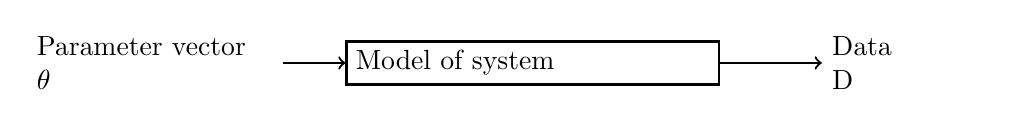
\begin{tikzpicture}[thick,scale=0.8]
\path[draw] % we place the nodes once
       node[text width=3cm] (1) at (0,0) {Parameter vector \\ $\theta$}  
       node[draw,text width=4.5cm] (2) at (6,0) {Model of system} 
       node[text width=2cm] (3) at (12,0) {Data \\ D} ;           

   \draw[->] (1) -- (2) ; 
    \draw[->] (2) -- (3) ;
    
   \end{tikzpicture}  \\

The model gives us the forward probability density of the outcome given the parameter, that is,  $P(D|\theta)$.   This density is the called the likelihood, although, as we see below, we don't usually consider it as a density in the usual way.

This model is not deterministic.  The data $D$ can be seen as a random sample from the probability distribution defined by the model (and parameters).  Changing the value of the parameters typically does not change the possible outcomes of the model but it  
will change the shape of the probability distribution, making some outcomes more likely, others less likely.



{\bf Example}: Suppose we are interested the number of buses stopping at a bus stop over the course of an hour.  We watch for the hour between 8am and 9am every weekday morning for  2 weeks.  We observe the outcomes  $D= (10 , 7 , 5 , 6 ,12 , 9 ,10 , 5 ,14  ,7)$.  A sensible model here might be the Poisson distribution where we say that the number of bus arrivals in an interval is Poisson distributed with parameter $\lambda$.  Our parameter vector contains just the single parameter $\theta = (\lambda)$ and our data vector contains the 10 observed outcomes $D = (D_1,D_2,\ldots,D_{10}) = (10 , 7 , 5 , 6 ,12 , 9 ,10 , 5 ,14  ,7)$.  

We derive the likelihood as follows.

The probability of observing the data $D$ for a given value of $\lambda$ is $P(D|\lambda)$. Let's assume that each observation is independent of others then $P(D|\lambda) = \prod_{i}P(D_i|\lambda)$.  That is, the probability of observing this series of outcomes is just the product of the probabilities of observing each particular outcome.  

The likelihood of a single observation is given by the probability distribution function for the Poisson since $D_i \sim Poiss(\lambda)$ so:   \[P(D_i|\lambda) = \frac{\lambda^{D_i}}{D_i!} e^{-\lambda}. \]
And so the likelihood of observing the full data $D$ is just 
\[
P(D|\lambda) = \prod_{i}P(D_i|\lambda) = \prod_{i}  \frac{\lambda^{D_i}}{D_i!} e^{-\lambda}. 
\]
\hfill $\square$


 
Note that the likelihood is a probability density function for $D$.  But $D$ is typically fixed in the sense that we make the observations which remain fixed through-out the analysis.  We will be interested in considering the likelihood as a function of the parameters $\theta$.  The likelihood is {\em not} a probability density function for $\theta$ since, in general $\int_{\theta \in \Theta} P(D|\theta) \, d\theta \neq 1$.

\subsection{Bayesian inference}

The statistical problem essentially comes down to one of observing the outcome, $D$ and wanting to recover the parameters $\theta$.  

That is, we want to estimate $\theta$ given $D$. We summarise our estimate of $\theta $ as a probability distribution, conditional on having observed $D$:    $P(\theta|D)$. This is called the {\bf posterior distribution} of $\theta$.  



From Bayes' theorem, we can express the posterior in terms of the likelihood:
\[ P(\theta|D) = \frac {P(D|\theta) P(\theta)}{P(D)}, \]
where $P(D|\theta)$ is the {\bf likelihood}, $P(\theta)$ is the {\bf prior distribution} of $\theta$ and $P(D)$ is a normalisation constant.

The prior $p(\theta)$ summarises what we know about a parameter before making any observations.

The posterior, $p(\theta | D)$ summarises what we know about $\theta$ after observing the data.

The likelihood tells us about the likeliness of the data under the model for any value of $\theta$. Recall that we consider the likelihood  a function of $\theta$ rather than a probability density for $D$; to emphasise this fact, people often write it explicitly as a function of $\theta$: $L(\theta) = P(D|\theta)$.

Bayes' theorem tells us how we update our beliefs given new data.  Our updated beliefs about $\theta$ are encapsulated in the posterior, while are initial beliefs are encapsulated in the prior.  Bayes' theorem simply tells us that that we obtain the posterior by multiplying the prior by the likelihood (and dividing by $P(D)$ which we can think of as a normalisation constant). 

Note that we need the normalisation constant as the posterior is a probability distribution for $\theta$, so its density must integrate to 1, i.e.,  $\int_{\theta \in \Theta} f(D|\theta) \, d\theta = 1$.  Thus the normalisation constant is $P(D) = \int_{\theta \in \Theta}  P(D|\theta) P(\theta) \, d\theta$. Typically this integral is hard to calculate so we try to find that will avoid having to calculate it.


{\bf Example}: In the example above, we found an expression for the likelihood.  To find an expression for the posterior, we need to decide on a prior distribution.  Suppose we had looked up general info about bus stops in the city and found that the busiest stop had an average of  30 buses an hour while the quietest had an average of less than 1 bus per hour.  We use  this prior information to say that any rate parameter $\lambda$ producing an average of between 0 ($\lambda = 0$) and 30  ($\lambda = 30$) buses an hour is equally likely.  This leads us to the prior $\lambda \sim U(0,30)$.  The density of this prior is $f(\lambda) = 1/30$ for $0 \leq \lambda \leq 30$.

To get the posterior density, we use the formula above: 
\[ f(\lambda | D) = \frac{f(D|\lambda)f(\lambda)}{P(D)} = \frac{ \prod_{i}  \frac{\lambda^{D_i}}{D_i!} e^{-\lambda} \frac{1}{30}}{P(D)}. \]
The normalisation constant $P(D)$ is the integral of the numerator over all possible values of $\lambda$:
\[
P(D) = \int_{0}^{30} \prod_{i}  \frac{\lambda^{D_i}}{D_i!} e^{-\lambda} \frac{1}{30} \, d \lambda.
\] \sqend

While it is possible to calculate this particular integral analytically, for most posterior distributions analytical integration is either very difficult or impossible.  We'll investigate methods for avoiding calculating difficult integrals like this in later sections.



\subsection{Maximum likelihood}

It is often difficult or inconvenient to deal with the posterior distribution (when the prior is hard to specify or the normalisation constant is impossible to calculate).   In these cases, we can still use our probabilistic model by concentrating solely on the likelihood function.  The aim here is typically to find the parameters that maximise the likelihood function.  That is, those parameters under which the observed data is most likely.  We call this parameter estimate the maximum likelihood estimate and write it as 
\[ \hat \theta  = \arg\max _\theta f(D | \theta) = \arg \max_\theta L( \theta;D)  \]
This function can be maximise using standard tools from calculus (taking the derivative and setting it to zero -- it is often easier to work with the log of the likelihood function as they both share a maximum) or using numerical techniques such as hill-climbing.  

Many methods in statistics are based on maximum likelihood including regression, $\chi^2-$tests, $t-$tests, ANOVA and so on.  

{\bf Example}: In the bus example above, we could find the maximum likelihood estimator for $\lambda$ by differentiating the log-likelihood, $\log(L( \lambda;D))$ with respect to $\lambda$, setting the result to zero and solving.  Note that we often work with  the log-likelihood rather than the likelihood for a couple of reasons: it is often easier algebraically and it helps avoid numerical under-flow  when the likelihood itself is very small.

\newpage
 
 \section{Simulation}

In a statistical setting there are a number of reasons we may wish to simulate from a distribution or a stochastic process.  We may wish to get a feeling for how the process behaves or estimate some quantity that we cannot calculate analytically.   An example of the latter case arises in Bayesian statistics, where the aim is to find the posterior distribution $f(\theta|x)$.  This can be very difficult for two main reasons:
\begin{itemize}
\item The normalising constant ($P(D)$, above)  involves a $p-$dimensional integral (where $p$ is the number of parameters of the model, that is, $\theta = (\theta_1,\theta_2,\ldots,\theta_p)$)  which is often impossible to calculate analytically.
\item Even if we are able to find $f(\theta|x)$, if we want to find the marginal distribution for some part of $\theta$ this may again involve a high-dimensional integral.
\end{itemize}
Both of these reasons boil down to the fact that integration is hard.  


To get around this problem, our approach will be to obtain a  sample of values,  $\{\theta^{(i)} \}$ for $i = 1,\ldots,n$, from the distribution of interest and use this sample to estimate properties of the distribution.  

For example, the mean of the distribution is $E[\theta]  = \sum_{\theta \in  \Omega} \theta \Pr(\theta)$.  We can estimate this from the sample set   by $E[\theta] \approx \bar{\theta} =  \frac1 n \sum_1^n \theta^{(i)}$.  This is called the sample mean of $\theta$, and is indicated by the bar over the variable.  The sample mean is an {\em estimator} of the mean.  More generally, we estimate the mean of a function of $\theta$ by $E[g(\theta)] \approx \bar g (\theta)  =  \frac1 n \sum_1^n g(\theta^{(i)})$.

How good are these estimates?  Since each sample $\theta^{(i)}$ is a random variable, $\bar g$ is a random variable.  That is, each time we obtain a different sample of values of $\theta$, we will get a different value for $\bar g$.    Clearly, as $n$, the size of the sample, increases our estimate will become more accurate but by how much?

It turns out that under quite general conditions, the main being that the samples, $\theta^{(i)}$ are independent of each other, $\bar g$ is normally distributed with mean $E[g]$ and variance $\mbox{var}(\bar g)  = \mbox{var}(g)/ n$.     When stated formally, this is known as a central limit theorem.  

Thus, if we have a method of simulating lots of independent samples, we can quickly get extremely accurate estimates of the quantities we are interested in.

Note that we can estimate more complex things than simple means using these methods.  For example, we can estimate the shape of distributions by drawing a histogram of the sampled points.  

So our attention turns to how we can generate this random sample.  First we consider how we can generate or simulate  randomness at all using (deterministic) computers.

\subsection{Random number generation}
\label{sec:rng}
All simulation relies on a ready supply of random numbers.   There are currently no known methods to generate truly random numbers with a computer without measuring some physical process.  There are, however, many fast and efficient methods for generating pseudo-random numbers that, for most applications, are completely sufficient.  The fact that these are based on algorithms that are repeatable makes them superior to physically based rngs for scientific simulation purposes.

We do not go into the mathematical details of pseudo-random number generators here as most major languages have libraries that implement perfectly adequate algorithms.  It is worth considering briefly what we want in a RNG.  The following quality criteria are taken from L'Ecuyer in the Handbook of Computational Statistics, 2004.  

The RNG must:
\begin{itemize}
\item have a very long period so that no repetitions of the cycle occur;
\item be efficient in memory and speed;
\item repeatable so that simulations can be reproduced;
\item portable between implementations;
\item have efficient jump-ahead methods so that a number of virtual streams of random numbers can be created from a single stream for use in parallel computations; and,
\item have good statistical properties approximating the uniform distribution on $[0,1]$.
\end{itemize}
It is relatively simple to come up with rngs that satisfy the first of these criteria, yet the last is where the difficulties occur.    The performance of rngs can be tested via  the diehard test suite (or more recently, the dieharder suite).  See \url{http://www.phy.duke.edu/~rgb/General/dieharder.php}.

%%%\notinexam{
\subsubsection{Linear congruential generators }

The most basic rngs are probably the linear congruential generators that have the form $X_{n+1} = (aX_n + b) \mbox{ mod }{m}$ where the constants $a, b$ and $m$ need to be chosen.   We divide the number by $m$ to get it in the range $[0,1]$, that is, set $U_i = \frac{X_i}m$.

These have poor statical properties, however, and should be avoided for simulations.

\subsubsection{Shift register generators}

All numbers in computers are stored as a group of bits (32 bits or 64 bits).  Shift register generators work directly with this representation to produce a sequence of random numbers.   Start with a seed $U_0 = 0.b_{01}b_{02}\ldots b_{0L}$ (where $L = 32$ or $L = 64$).  Then get $U_i = 0.b_{i1}b_{i2}\ldots b_{iL}$ by $b_{ij} = f_j(b_{(i-1)1},b_{(i-1)2},\ldots,b_{(i-1)L})$ where $f_j$ is some function  $f: \{0,1\}^L \rightarrow \{ 0,1\}$.  

Example: For $L = 4$, set $f_1 = b_{(i-1)3} \, \mathrm{XOR} \, b_{(i-1)4}$ and $f_j = b_{(i-1)(j-1)}$ otherwise.  Starting with $0101$ we get the following sequence:

\begin{verbatim}
0101
1010
1101
1110
1111
0111
0011
0001
1000
0100
0010
1001
1100
0110
1011
0101
\end{verbatim} \hfill $\square$


An rng that extends this idea is the so-called  Mersenne Twister which is the statisticians rng of choice for simulation.   Most languages have an implementation of this algorithm.  See the  wikipedia page \url{http://en.wikipedia.org/wiki/Mersenne_twister} for more details.

The Mersenne Twister is implemented in the Colt library for Java (see \burl{https://acs.lbl.gov/software/colt/}).  It is the default rng in the Python random library.


%%}%end not in exam

\subsection{Simulating from univariate distributions via Inversion sampling}

 Simulation from discrete or continuous distributions with cumulative density function $F(X)$ relies on the following result which tells us that all we need to simulate draws from  an arbitrary univariate distribution is a draw from  $U(0,1)$ and use the inverse of the cdf:

{\bf Result (Inversion method):} If  $U \sim U(0,1)$, then $X =  F^{-1}(U)$ produces a draw from $X$ where $F^{-1}$ is the inverse of $X$. 

Thus when the cdf is known and we can find the inverse, sampling from the distribution is easy, as the following example shows.

{\bf Example (simulating an exponential random variable)}:  if $X \sim \mbox{Exp}(\lambda)$, then $F(x) = \int_{-\infty}^x f(t) dt =  \int_{-\infty}^x \lambda e^{-\lambda t} dt = 1-e^{-\lambda x}$. 

 It is simple to see (by setting $u = 1-e^{-\lambda y}$ and solving for $y$)  that $F^{-1}(u) = - \log(1-u)/\lambda$. 
  
 Since $1-U \sim U(0,1)$ when $U \sim U(0,1)$, we can use this expression to generate exponential random variables by generating the uniform random variable $u$ and setting $x = - \log(u)/\lambda$. \hfill $\square$

\begin{figure}
\centering
\includegraphics[width = 8cm]{figures/inversionsample.pdf}
\caption{Sampling an $Exp(1)$ random variable using the inversion method.  A uniform sample $u \sim U(0,1)$ is drawn.  Here $u = 0.72$ shown on the vertical axis.  This is mapped, via the cdf, to $x \sim Exp(1)$ to produce $x = -\log(1-u) = 1.272$ shown on the horizontal axis. }
\end{figure}

Note that with discrete random variables, a  inverse of $F$ is ambiguously defined (since $F$ is a step function).  It is possible to extend the definition of an inverse to derive the following method for simulating discrete random variables.



{\bf Inversion sampling from a discrete distribution}: If $X$ is discrete with  $P(X = x_i) = p_i$, we generate $U \sim U(0,1)$ and set $X = x_1$ if $u< p_1$ and $X = x_i$ if $\sum_{j = 1}^{i-1}p_j < u < \sum _{j = 1}^i p_j$.

{\bf Example:} Use the inversion method  to obtain samples from $X \sim Binomial($n = 5, p = 0.3$)$.

{\bf Solution:} The possible values $X$  can take are $(0,1,2,3,4,5 )$ with probabilities $f(x) = (  0.168, 0.360 ,0.309 ,0.132 ,0.028, 0.002)$, respectively (from Section \ref{sec:binom}).  Obtain the cdf by taking the cumulative sum of these probabilities:  $F(X) = ( 0.168, 0.528, 0.837 ,\\0.969, 0.998 ,1.000)$.  Now obtain samples from $X$ by sampling $u \sim U(0,1)$ and finding the index of the smallest value of the cdf which is larger than $u$.  E.g. if $u = 0.439$, $x = 1$ since $F(0) = 0.168 < u < F(1) = 0.528$,  Similarly,  if $u = 0.972$, $x = 4$ since $F(3) < u < F(4)$.\sqend



\newpage

\subsection{Stochastic processes}

So far we have talked about random variables which can be pretty much any object but are only observed at one time. A stochastic process is a collection of random variables that describes the evolution of a system that is subject to randomness.   A stochastic process could, for example, describe the position of a particle that is being buffeted by other particles, the state of a genetic sequence that is subject to copying with mutation, or the shape and size of a land mass that is subject to geological forces.  

Mathematically, we consider a random process $X$ as the set of random variables $\{X_t: t \in T\}$ where $T$ is some index set, such as discrete time ($T = 0,1,2,\ldots$) or continuous time ($T = [0,\infty)$). 

We will try to get an understanding of these process by studying a few examples. 

\subsubsection{Random walk}

One of the simplest stochastic processes is known as the simple symmetric random walk, or drunkard's walk.  Imagine a person leaves the pub so drunk that their method of getting home consists of taking random steps, with probability 0.5 the step is in the direction of home with probability 0.5 it is in the other opposite direction.   We can model the drunk's position after the $i$th step as a random variable $X_i$ where $X_0 = 0$ (that is, the pub is the origin).   Then $X_{i+1} = X_i + S_{i}$ where 
\[S_{i} =   
\begin{cases}
   +1  & \mbox{with probability } 1/2 \\
   -1    &  \mbox{with probability }  1/2.
  \end{cases}
 \] with is the direction of the $i$th step.  Equivalently, $X_i = X_0 + \sum_{j = 0}^{i-1} S_j.$  
The process, while amenable to analytic techniques, is extremely simple to simulate: we just need to be able to simulate Bernoulli random variables.  



The random walk has many variations: instead of looking at a symmetric walk, consider $S_i = 1$ with probability $p$; we can consider the random walk in higher dimensions, choosing from $2^d$ possible directions in $d$ dimensions; and choosing a different step size ($S_i = \pm c$, say).

The process has some very nice, and often surprising, properties.  For example, the simple symmetric random walk crosses every point an infinite number of times (this is known as Gambler's ruin, as if $X$ models the amount a gambler is winning when betting \$1 on toss of a coin, the gambler will certainly eventually lose all their money if they play for long enough against a casino with infinite resources).  

Secondly, the random walk in $d$ dimensions returns to the origin with probability $1$ for $d = 1,2$, but for $d\geq 3$, that probability is below 1 (about 0.34 in for $d = 3$, 0.19 for $d = 4$ etc.).

% Expected value of $X$ after $n$ steps of size $c$ when $\Pr(S_i = +c)  = p$ is  $E[X_n] = nc(2p-1)$ and variance is $\var[X_n] = 4nc^2p(1-p)$.


\subsubsection{Poisson process}

The Poisson process is a simple yet incredibly useful model for events that occur independently of each other and randomly in time (or space).    It is commonly used to model events such as:
\begin{itemize}
\item Genetic mutations
\item arrival times of customers
\item radioactive decay
\item occurrences of earthquakes
\item industrial accidents
\item errors in manufacturing processes (e.g. silicon wafers or cloth)
\end{itemize}
We will consider processes in time although the concepts extend readily to space (the last of the examples above could be spatial).

A Poisson process is sometimes called a {\em point process}.  It is counts the number of events in the time interval $[0,t]$.  Let $N(t)$ be the number of points in the interval, so that $N(t)$ is a counting process.

Define a {\em Poisson process with intensity $\lambda$}, where $\lambda > 0$ (also called the {\em rate}) to be a process $\mathbf N = \{ N(t), t \geq 0 \} $ that takes values in $S = \{0,1,2,\ldots \}$ that satisfies the following properties:
\begin{enumerate}
\item $N(0) = 0$ and if $s < t$ then $N(s) < N(t)$.
\item If $s < t$ then $N(t) - N(s)$ is the number of arrivals in $(s,t]$ which is independent of the number (and times) of the arrivals in $(0,s]$.
\item \[ \Pr(N(t+h) = n+m | N(t)  = n) = 
\begin{cases} \lambda h + o(h) & \mbox{ if } m = 1 \\
o(h) &  \mbox{ if } m >1 \\
 1 - \lambda h + o(h) &  \mbox{ if } m = 0.
 \end{cases}
\]
\end{enumerate}
Here the notation $o(h)$ indicates that, as $h$ gets small the bit of the expression that is $o(h)$ disappears.  A strict definition is that  function $f$ is $o(h)$ (`of order little oh of $h$') if \[ \lim_{h \rightarrow 0} \frac {f(h)}h = 0.\]
Examples: Check that $f(h) = h^2$ is $o(h)$ while $f(h) = h^{-\frac 12}$ is not. \hfill $\square$


The Poisson process is related to the Poisson distribution by the fact that $N(t)$ has a Poisson distribution with parameter $\lambda t$ so that \[\Pr(N(t) = k) = \frac{(\lambda t)^k}{k!} \exp(-\lambda t)\]
for $k \in \{0,1,2,\ldots\}$.  



Now look at the  times between events in a Poisson process. Let $T_i$ denote the time of the $i$th event of the process and $T_0 = 0$.  Then the $i$th {\em inter-arrival time}, $X_i = T_{i+1} - T_{i} $, is exponentially distributed with parameter $\lambda$, that is $X_i \sim \mbox{Exp}(\lambda), \, i = 1,2,3,\ldots$.
 
 
Poisson processes have some very nice properties.  

{\bf Splitting:} Let $\{N(t),t \geq 0\}$ be a Poisson process with rate $\lambda$. Suppose each event is of type $i$, for $i \in \{1,\ldots,k\}$ with probability $p_i$ and suppose that this is independent of other events.

If we observe just the events of type $i$, they form a Poisson process with rate $\lambda p_i$ independently of the remaining types of events.

For example, if we look at the request for different types of data in a network or arrivals of different types of customer, we get the large Poission process separated out as multiple smaller (lower rate) Poisson processes.


{\bf Merging:} The converse of splitting is merging:   Let $N = \{N(t),t \geq 0\}$ be a Poisson process with rate $\lambda$ and $M = \{M(t),t \geq 0\}$ be a Poisson process with rate $\mu$ independent of $N$.
Then $L = \{L(t) = N (t) + M (t), t \geq 0\}$ is a Poisson process of rate $\lambda + \mu$.



Together, these results tell us how to model multiple Poisson processes using a single large process:  Suppose we have $n$ independent Poisson processes where process $i$ has rate $\lambda_i$.  Then the  merged process has events of $n$ different types. If we observe an event in the merged process, let $p_i$ be the probability of the event being of type $i$.  What is $p_i$?   

According to the splitting theorem, the type $i$ process has rate $\lambda_i = \lambda p_i$ where $\sum_i p_i = 1$ so that $\lambda = \sum_i \lambda_i$. So $p_i$ is given by
\[ p_i = \frac{\lambda_i}{\lambda} = \frac{\lambda_i}{\lambda_1 + \ldots + \lambda_n} = \frac{\mbox{rate of type }i}{\mbox{total rate}}.\]

{\bf Example}: We model arrivals at a bus stop as a Poisson process.  Some people arriving are students and some are office workers.  Students arrive at rate $\lambda_1$, office workers arrive at rate $\lambda_2$.  Merging these processes tells us the total rate of arrivals is $\lambda_1+\lambda_2$.  The probability that any given   arrival is a student is $\frac{\lambda_1}{\lambda_1+\lambda_2}$ while the probability that they are an office worker is $\frac{\lambda_2}{\lambda_1+\lambda_2}$. \hfill $\square$



\section{Markov chains}

We think of a random process as a sequence of random variables $\{X_t: t\in T \}$ where $T$ is an index set. $T$ can be thought of as time.   If $T$ is discrete, the process $X(t)$ is called a {\em discrete time random process} while if $T$ is continuous, $X(t)$ is called a {\em continuous time random process}.    The random walk example is an example of a discrete time process (each time unit corresponds to a single step in the process) while the Poisson process is a continuous time process (arrivals happen at any time).  We will consider only discrete time processes until further notice.


The random walk and Poisson processes described above both share an important property, known as the Markov property.  Intuitively, this is the property of memorylessness in that future states depend only on the current state and not any past states.  That is, to propagate the process forward, we need only be told the current state to generate the next state.  


Formally, the sequence of random variables $X_1,X_2, X_3,\ldots$ is a {\em Markov chain} if it has the {\em Markov property}:   
\[P(X_{n+1} = x | X_n = x_n, X_{n-1} = x_{n-1},\ldots,X_2 = x_2,X_1=x_1) = P(X_{n+1} = x |X_n = x_n).\]

Markov chains are commonly used to model processes that are sequential in nature and where the  future state only depends on the current state.  This limited dependence property is called the Markov property (after Andrey Andreyevich Markov, a Russian mathematician from the late 19th century).  

\begin{description}
\item[Example 1:] The random walk.  Start at $X_0 = 0$.  If  $X_n$ is the current state, $P(X_{n+1} = X_n+1 | X_n) = 1/2 = P(X_{n+1} = X_n-1 | X_n)$.   This is a Markov chain on an infinite state space.  A realisation of this chain: 0 1  0 -1  0  1  2  3  2  1  2  1  2  1  0  1

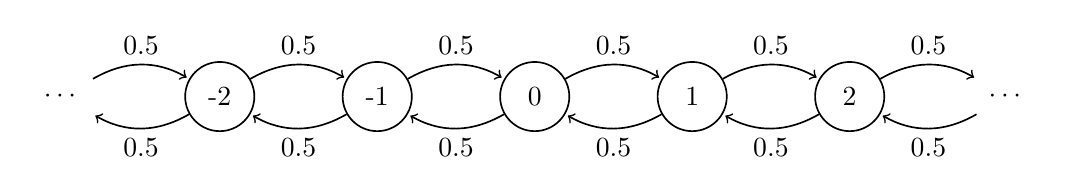
\begin{tikzpicture}[->,shorten >=1pt,auto,node distance=2cm,
                    semithick,every text node part/.style={align=center}]
  \tikzstyle{every state}=[fill=none,draw=black,text=black]
  
  \node[state,draw = none] (m3)                    {$\cdots$};
  \node[state] (m2)        [right of=m3]              {-2};
  \node[state]         (m1) [right of=m2] {-1};
  \node[state]         (m0) [right of=m1] {0};
  \node[state]         (p1) [right of=m0] {1};
  \node[state]         (p2) [right of=p1] {2};
  \node[state,draw = none]         (p3) [right of=p2] {$\cdots$};

  \path (m3) edge    [bend left]          node {0.5} (m2)
           (m2) edge    [bend left]          node {0.5} (m1)
           (m1) edge    [bend left]          node {0.5} (m0)
           (m0) edge    [bend left]          node {0.5} (p1)
           (p1) edge    [bend left]          node {0.5} (p2)
           (p2) edge    [bend left]          node {0.5} (p3)
           (p3) edge    [bend left]          node {0.5} (p2)
           (p2) edge    [bend left]          node {0.5} (p1)
           (p1) edge    [bend left]          node {0.5} (m0)
           (m0) edge    [bend left]          node {0.5} (m1)
           (m1) edge    [bend left]          node {0.5} (m2)
           (m2) edge    [bend left]          node {0.5} (m3);
 \end{tikzpicture}


\item[Example 2:] Weather.   The weather tomorrow depends on the weather today.  If it is sunny today, tomorrow it is sunny with probability 0.7 and rainy otherwise.  Rain clears a bit faster, so if it is rainy today, it is rainy tomorrow with probability 0.6 and sunny otherwise.  This is a Markov chain with state space $\{ R,S \}$ (for rainy and sunny, respectively).  The following is a simulated realisation: S S S S S S R S R R R

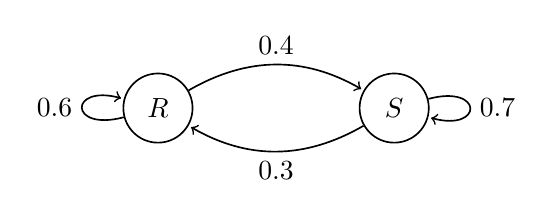
\begin{tikzpicture}[->,shorten >=1pt,auto,node distance=3cm,
                    semithick,every text node part/.style={align=center}]
  \tikzstyle{every state}=[fill=none,draw=black,text=black]

  \node[state] (R)                    {$R$};
  \node[state]         (S) [right of=R] {$S$};

  \path (R) edge    [bend left]          node {0.4} (S)
        (R) edge [loop left] node {0.6} (R)
        (S) edge    [bend left]          node {0.3} (R)
        (S) edge [loop right] node {0.7} (S);
 \end{tikzpicture}



\item[Example 3:]  The following is {\bf not} a Markov chain. Recall our random walk is called a drunkard's walk.  Imagine someone occasionally  helps the drunkard on the way home by carrying him 10 paces either to the left or the right.   This person has limited patience, though, so will help at most 3 times.  When the person has not  yet reached the limit of their patience, possible transitions include
$X_{n+1} = X_n \pm 10$ or $X_{n+1} = X_n \pm 1$.  After the person has intervened to help 3 times, the only possible transitions are $ X_{n+1}  = X_n \pm 1$.  So to see if this large movement is possible, we need to look back in history to see how many interventions have occurred.  Thus the distribution of the next state depends on more than just the current state and the chain is not a Markov chain. \hfill $\square$
\end{description}



The chain is {\em homogeneous} if $\Pr(X_{n+1} = j|X_n = i) = \Pr(X_1 = j|X_0 = i)$. If a chain is homogeneous, we write $P_{ij} = \Pr(X_1 = j|X_0 = i)$.  The transition probabilities are normalised so that $\sum_j P_{ij} = 1$. 

The matrix $P = [P_{ij}]$ is called a {\em stochastic matrix} as all its entries  are non-negative and its rows sum to 1, so that $\sum_j P_{ij} = 1$.


{\bf Example}: The transition matrix for the weather example given above is 
$\left[ \begin{array}{cc} 0.7 & 0.3 \\
0.4 & 0.6 \end{array} \right] $
where rows and columns 1 and 2 are indexed by $S$ and $R$, respectively. \hfill $\square$

A homogeneous Markov chain is completely defined  by specifying  an initial distribution $\Pr(X_0 = i)$ for $X_0$ and the transition probabilities $X_{n+1}$ given $X_n$, $P_{ij}$.  
 
 

\begin{description}

\item[Example 4:] Music.  See Figure \ref{fig:lydia}. This example taken from  Tom Collins, Robin Laney, Alistair Willis, and Paul H. Garthwaite. Chopin, mazurkas and Markov. Significance, 8(4):154-159, 2011. \href{http://onlinelibrary.wiley.com/doi/10.1111/j.1740-9713.2011.00519.x/pdf}{doi:10.1111/j.1740-9713.2011.00519.x}.

\begin{figure}[hbtp]
\includegraphics[width=14cm]{figures/lydia}
\includegraphics[width=14cm]{figures/matrixlydia}
\includegraphics[width=5cm]{figures/randomlydia}
\caption{An example showing how a piece of music can be modelled as  a Markov chain.  The original piece, a fragment of  Lydia by Faur\'e, is shown at the top.  Just the pitches are considered in this simple Markov model.  The transition matrix between pitches (centre) is constructed from empirical counts of the observed transitions.  Three random realisations of the process are given at the bottom.  }
\label{fig:lydia}
\end{figure}

\item[Example 5:]  A DNA sequence.  State space is $\{A,C,G,T \}$.  Need to specify transition probabilities $P_{AA}, P_{AC}, P_{AG}$ etc.  Then we obtain a random sequence by specifying a starting state and recording each state visited.    An example of a random sequence looks as follows: AAGCTGCGTGTGGGGGAAGGAACTTTTGCGTGTTAGTA
\end{description}


 The {\em $m-$step transition probability} is the probability of going from state $i$ to state $j$ in exactly $m$ steps, $P_{ij}(m) = \Pr(X_{n+m} = j|X_n = m).$   
Hence the  $m-$step transition  matrix is $P_m = [P_{ij}(m)]$. 
  
A result known as the {\em Chapman-Kolmogorov equations} tells us $P_{m+n} = P_mP_n$ (where the right-hand side is just standard matrix multiplication). In particular, this result tells us that $P_n = P^n$, that is, the n-step transition matrix is just the $n$th power of the (one-step) transition matrix. 

\newpage
 
\section{Introduction to genetics and genetic terminology }

The history of life can be viewed, in a rather mundane way,  as a long running and very complex stochastic (or random) process.

At a very basic level, and after many simplifying assumptions, we can think of the historical process explaining the relationships between species as a tree.   The points where the tree splits are speciations and the leaves of the tree are different  species.  The past is back at the base or root of the tree and time increases from the root to the tips.  Information is passed along  the tree (away from the root) from one generation to the next via genetic material.

Genetic material is thought to be the only means by which biological information is passed from parent to offspring.  The process of copying genetic material is imperfect, so that children will differ slightly from the parent.  These imperfections consist of errors in the copying, known as mutations, and can be thought of as a stochastic process.

The fundamental objects we will be studying are sequences of characters representing biological macromolecules: DNA (Deoxyribonucleic),   RNA  (Ribonucleic acid) and proteins.  DNA are RNA are the primary forms of genetic material.    The characters in DNA and RNA sequences are drawn from 4 letter alphabets: DNA has $\Omega = \{A,C,G,T \}$ while RNA has $\Omega = \{A,C,G,U \}$.  The A stands for adenine, C for cytosine, G for guanine, T for thymine and U for uracil. These are known as nucleobases or simply bases, with $C,T,U$ being {\em pyramidines } and $A,G$ being {\em purines}.    Protein sequences consist of the twenty amino acids that are represented by the alphabet $\{ A,R,N,D,C,E,Q,G,H,I,L,K,M,F,P,S,T,W,Y,V\}$ (that is, all the letters except $\{ B,J,O,U,X,Z \}$). We will refer to the bases in an DNA/RNA sequence or the amino acids in a protein sequence as {\em residues}. 

In eukaryotes (organisms with cells that  have a nucleus), the three types of sequences related to each other by the Central Dogma of  Molecular Biology that states, DNA makes RNA makes Protein.  Or, more prosaically,   DNA is {\em transcribed} into a type of RNA called mRNA that is then {\em translated} into protein.  

There are some good animations showing how translation and transcription work at \url{www.hhmi.org/biointeractive/animations/index.html}, in particular see the DNA transcription and translation animations.  A Japanese anime style film of the central dogma is also worth a look: \url{http://www.youtube.com/watch?v=-ygpqVr7_xs}. 

Parts of the the DNA sequence encode information for proteins.  These regions are known as genes and must be transcribed to RNA before being built into proteins.  When the DNA is transcribed to RNA, all bases are copied exactly except that $T$ (thymine) is transcribed as $U$ (uracil).  Once copied, the RNA is edited at splice sites so that only exons remain (the introns are edited out).  This leaves the {\em messenger RNA}, mRNA, which is then  translated to a protein sequence (poly-peptide chain).  This translation  occurs via the genetic code which translates consecutive triples of RNA bases (known as a codon) into one of the 20 amino acids.  There are $4^3 = 64$ possible codes since there is an alphabet of 4 bases.  60 of these code for proteins, 1 (AUG) is a start codon and 3 (UAA, UGA and UAG) are stop codons signalling the start or finish of a protein.  A particular  amino acid may be encoded by just one codon (e.g. AUG$\rightarrow$Methionine(M)) or up to 6 (e.g. any of  UUA, UUG, CUU, CUC, CUA, CUG$\rightarrow$Leucine (L)).    Once the poly-peptide chain is formed it folds into three dimensional molecule, taking on a particular structure.

{\bf Example:} The sequence {\tt atgaggttgacgctactttgttgcacctggagggaa} can be split into codons {\tt atg agg ttg acg cta ctt tgt tgc acc tgg agg gaa} which translate into the protein sequence {\tt MRLTLLCCTWRE}. \sqend

In this course, we are only interested in the primary structure of sequences, that is, the order in which residues occur along the sequence.  We will ignore the secondary, tertiary and quaternary structure of proteins ---  secondary structure is the name for  the regular substructures such as alpha helices and beta sheets, the tertiary structure are the three dimensional structures of single molecules while quaternary structure are the complex forms taken by collections of single protein molecules.  The study of these more complex structures is known as structural bioinformatics.

When DNA is passed from one generation to the next, the copy made is not exact.    There are a number of processes that cause differences to arise between the parent and child.  Recombination is one such process and involves the mixing of the maternal and paternal copies of DNA when the gametes (eggs or sperm) are produced.  Other processes are generally thought of as mutations.  The simplest are {\em point mutations} where the offspring sequence differs from the parent sequence by a single base (residue).  This type of mutation is called a {\em single nucleotide polymorphism}, abbreviated as SNP and pronounced `snip'.   {\em Insertions} (or deletions) refer to the child sequence gaining (losing) one or more base than the parent.  Larger scale mutations include: {\em gene duplication} which is a large scale  insertion where the child inherits  extra copy of a region containing a whole gene.  Other large scale  mutations include inversions (part of the sequence is reversed end to end) and translocations (a piece of the sequence is copied out of order).


{\bf Examples of mutations}: Consider the short sequence 
{\tt cgctcaccatgaagcgtttcactaat}.  We demonstrate types of mutations showing the original sequence and a mutated version of it below with X marking the mutation.
\begin{itemize}
\item Single nucleotide polymorphism (SNP) \\
{\tt cgctcaccatgaagcgtttcactaat}\\
{\tt cgctcgccatgaagcgtttcactaat}\\
{\tt .....X....................}
\item Insertion \\
{\tt cgctcacc----atgaagcgtttcactaat}\\
{\tt cgctcacctgatatgaagcgtttcactaat}\\
{\tt ........XXXX..................}
\item Deletion \\
{\tt cgctcaccatgaagcgtttcactaat}\\
{\tt cgct----atgaagcgtttcactaat}\\
{\tt ....XXXX..................}
\item Duplication (the copied region is marked with parentheses).  Note that duplication usually refers to gene duplication where whole genes are copied. \\
{\tt cgctcaccatgaagcgtttcacta-----------at}\\
{\tt cgctcaccatgaagcgtttcactacaccatgaagcat}\\
{\tt ....(.........).........XXXXXXXXXXX..}
\item Inversion (again, this typically happens at a larger scale than shown here) \\
{\tt cgctcaccatgaagcgtttcactaat}\\
{\tt cgctctaccagaagcgtttcactaat}\\
{\tt .....XXXXX................}

\end{itemize} \sqend

 

All these processes can be modelled and studied, with varying degrees of difficulty.  We'll focus primarily on the question of how to align the sequences, how to identify regions of interest in sequences (for example, genes), and given aligned sequences, how can we reconstruct the evolutionary history (the tree) of those sequences.  This last problem will require us to model the the mutation process where we restrict ourselves to looking at how point mutations arise.

The models we use will use are relatively simple, sometimes to the point of being downright crude.  It is good to keep in mind the quote from the famous statistician George Box who said, ``All models are wrong but some are useful''.

\subsection{Summary of above} 
\begin{itemize}
\item We model genetic sequences: think of them as strings of letters.
\item There are 3 types of sequence, DNA, RNA or Protein.
\item DNA sequences are composed of the 4 letters, or bases, $ \{A, C, G, T \}$,  RNA is made of the bases $\{A,C,G,U\}$ while protein sequences are made up of the 20 amino acids. 
\item The three types of sequence are related by the central dogma of molecular biology: DNA is transcribed to RNA and then translated to protein.  
\item Protein sequences fold up into more complex structures.  We will ignore this structure in this introductory course.
\item DNA is copied from parent to child.  
\item At copying, mutations are introduced. 
\item Mutations may be single nucleotide polymorphisms (SNPs), insertions, deletions or of other types.
\item We use a tree to  model the history of relationships between individuals (which are represented by their sequences).
\end{itemize}


To model  the complex random process of genetic mutation and inheritance, we will need  tools from applied probability and statistics.  The next few sections are concerned with introducing the main tools and concepts that we will use for our study.  All of you will have previously encountered at least some of the ideas we discuss here  but, as with the linear algebra sections, it helps to review the main points before plunging in to new material.

%\end{document}

\section{Alignment}

\subsection{Homology}

Homology (from the Greek, to agree) is a crucial concept in biology referring to traits or, in the case of sequences,  sequence regions  that share a common ancestry.  We expect homologous regions to be similar to each other where the level of similarity will depend on how recently they shared a common ancestor.

Thus to say two regions are homologous is an evolutionary hypothesis.  Mrs Darwin (in Carol Ann Duffy's poem from the collection The World's Wife) was making an evolutionary hypothesis of homology:

7 April 1852 \\
Went to the Zoo.\\
I said to Him --- \\
Something about that Chimpanzee over there reminds me of you.

The claim does not imply that the regions share a similar function now or, depending on the time since divergence, that they  even particularly similar, just that they share a common ancestor.  Therefore, sequences are either homologous or not, there are no degrees of homology. We often infer homology between two sequences when they are similar but we must be careful as we can get similarity without homology.  Homologous sequences are sometimes referred to as {\em homologs}.

There are two main ways that we get similarity without homology: either by chance or by convergent evolution.  Similarity by chance will occur even in completely random sequences on a finite alphabet.  In two random sequences of four letters, we would expect similarity by chance of 25\%.  

Convergent evolution occurs when similar functions evolve independently of each other.  An example of this are the wings of birds and insects.  We don't believe these two very different creatures had a common ancestor that evolved wings but that wings evolved indecently of each other in the insect and bird lineages.  Thus, while wings in a fly and a sparrow may be superficially similar, they are not considered homologous.  The same applies to sequences that code for similar proteins (i.e., have similar function) but have evolved independently.  Such traits/regions are called analogous.

We distinguish between two types of homology: orthology and paralogy:
\begin{description}
\item[Orthology] occurs when two genes are separated by a speciation event and evolve independently from there on.   
\item[Paralogy] occurs when a region of the genome is duplicated in the same genome (a duplication event) and they evolve in parallel in the same genome.  The two copies are said to be paralogs.
\end{description}


\subsection{Pairwise alignment}



Given two sequences, if they are homologues, how do they align with each other?  That is, exactly which sites in the sequence are homologous with each other?  

We consider pairs of sequences, $x$ and $y$ of length $m$ and $n$, respectively. $x_i$ is the $i$th symbol of $x$. These symbols are usually the 4 DNA or RNA bases or the 20 amino acids. We refer to the symbols as {\em  residues}.

We will allow {\em gaps} to be introduced in either sequence to allow them to align better.   Biologically, gaps correspond to insertions or deletions in the sequence.

Clearly, there are many ways of aligning a pair of sequences (how many?), but what is the best alignment?

Example: x = GAATTC and y =  GATTA 
\begin{verbatim} 
GAATTC or GAATTC-
GA-TTA    -GATT-A
\end{verbatim}
are two possible alignments. \hfill $\square$

\subsection{Scoring alignments}

The best alignment will depend on how we score alignments.  It is easy to come up with different scoring regimes (e.g., score 1 for a match, -1 for a mismatch) but we really want to compare two models --- that the similarity we see is just chance vs. that the sequences are homologs. 

We initially consider alignments without gaps.

\subsubsection{Model of non-homologous  sequences}

The most basic model is that each letter appears with some probability, letter $a$ appears with probability $q_a$ (note that the probabilities summed over the alphabet are 1), that each site is independent and that the each sequence is independent. Then the probability of seeing sequence $x$ is
\[ P(x) = \prod_{i = 1}^n q_{x_i} \]
and the joint likelihood of an alignment is just the joint probability of the sequences $x$
and $y$,
\[ P(x,y) = P(x)P(y) = \prod_{i = 1}^n q_{x_i} \prod_{i = 1}^m q_{y_i} = \prod_{i = 1}^n q_{x_i}q_{y_i}.  \]




\subsubsection{Model  of homologous  sequences}


An alternative model is that the two sequences are related and the probability of seeing
the pair of residues $a$ (from $x$) and $b$ (from $y$) aligned at a locus is $p_{ab}$. The probability of the alignment is then the product of the loci,
\[ P(x,y) = \prod_{i = 1}^n p_{x_iy_i}. \]


To compare these two models, we take ratio of these likelihoods:
\[ \frac{\prod_{i=1}^n p_{x_iy_i}}{ \prod_{i = 1}^n q_{x_i}q_{y_i}} = \prod_{i = 1}^n \frac{ p_{x_iy_i}}{q_{x_i}q_{y_i}}. \]
It is easier to work with log-likelihoods (and addition) than likelihoods and multiplica- tion, so we take the log of this quantity to get
\[ S= \sum_i s(x_,y_i) \]
where
\[ s(a,b) = \log\left(\frac{p_{ab}}{q_aq_b}\right).\]
The score of the alignment then is the sum over the local score $s(a, b)$. $s$ can be thought of as a matrix and is often referred to as a {\em score matrix } or {\em substitution matrix}. 


There are various methods for deciding reasonable values for the entries of the matrix, discussed below.
Note that even when ad hoc values are chosen for the matrix, the underlying probabilities, $p_{ab}$ and $q_a$ can be derived by reversing the above argument.  That is, when a score matrix is selected we are making implicit assumptions about the $q_a$s and $p_{ab}$s.

Example: If x = GAATTC and y =  GGATTA are aligned as 
\begin{verbatim} 
GAATTC
GGATTA
\end{verbatim}
where $s(a,b) = 2$  if $a = b$ and $s(a,b) = -1$ if $a \neq b$, the alignments scores $2-1+2+2+2-1 = 6$. \hfill $\square$



\subsection{Choosing the substitution matrix}

For protein sequences, the quantities $p_{ab}$ and $q_a$ have been empirically estimated to produce score matrices.  In particular, the  BLOSUM (BLocks SUbstitution Matrix) matrix of which there are various types, e.g. Blosum 45 and Blosum 80.

These matrices were calculated by studying a large number of confirmed alignments where there was considerable agreement between the sequences. The relative frequency of residues was calculated (to estimates for  the $q_a$s.) and the relative frequencies of pairs of residues was calculated  (to give estimates for  the $p_{ab}$s). The relative frequencies were then scaled to give integer entries in the matrix.  The number after the matrix represents the similarity of the sequences used to estimate the matrix, so matrices with higher numbers are used for less divergent sequences.  

The Blosum matrices are generally the most effective and widely used but see also PAM  (Point Accepted Mutation) matrices. 
%For more information, see \url{http://www.ebi.ac.uk/help/matrix.html}.


\begin{figure}[hbtp]
\includegraphics[width=14cm]{figures/blosum45}
\caption{The Blosum 45 score matrix.  The matrix is symmetric as $s(a,b) = s(b,a)$.  }
\label{fig:blosum}
\end{figure}



%
%x = TTCATA and y = TGCTCGTA
%gives 
%\begin{verbatim}
%T--TCATA
%TGCTCGTA
%\end{verbatim}
%
%
% How do we deal with gaps in the alignment?
 
\subsubsection{Scoring gaps}

To make sequences align fully, we add gaps to one sequence or the other.  A gap in $x$ corresponds to an insertion in $y$ with respect to $x$ or a deletion in $x$ with respect to $y$.    Adding gaps comes with a penalty, so reduces the score for the match. 

For a gap of length $k$, write  $\gamma(k)$ for the penalty.  We consider two forms for $\gamma$. 

A {\em  linear penalty } is defined by $\gamma(k) = -dk $ for some $d > 0$.  That is, each deleted base adds a penalty of $d$.

 An {\em affine penalty} is defined by $\gamma(k)= -d-(k-1)e$ where $d>e>0$. $d$ is the gap open penalty and $e$ is the gap extension penalty.  The affine penalty is more biologically appropriate as insertions or deletions are typically created in a single event rather than building up one residue at a time. 
 
 
More complex gap penalties can be used, for example, we may wish to have different penalties for gaps matched with different residues, or non-linear functions of gap length.   Such penalties come at the cost of more difficult implementation.

In the algorithms below, we'll first consider the  simple case of  the linear penalty.


\newpage


\subsection{Global alignment: Needleman-Wunsch algorithm}

We can't calculate all possible alignments of a pair of sequences. (There are ${n+m \choose m}$ possible  alignments for a pair of sequences of length $n$ and $m$.) We use {\em dynamic programming}  approaches that allow is to quickly calculate the best possible alignment (that is, the one that gives us the highest score).  

Dynamic programming is technique of solving   complex problems by reducing them to a number of  much simpler subproblems that  we can easily solve then re-assemble to find the answer to the complex problem.  It uses the structure of the problem itself and so is only applicable to problems that possess a certain type of structure and to which we can apply the Principle of Optimality: ``a sub-optimal solution of a sub-problem cannot be part of optimal solution of original problem''.

The the alignment context, the principle of optimality holds in that if we know the score of an  optimal alignment of length $k$ then the score of the first $k-1$ parts of the alignment must be optimal. 


To see why this is, let  $F_{i,j}$ be the score of the optimal alignment between $x[1 : i]$ and $y[1 : j]$.  Let  $s(x_i,y_j)$ be the score for matching residue $x_i$ to residue $y_j$ and assume a linear gap penalty (so that the penalty for adding the gap $(x_i, -)$ or $(-,y_j)$ is $d$).  The optimal alignment up to $x_i,y_j$ either has $x_i$ and $y_j$ aligned, or $y_j$ aligned to a gap or $x_i$ aligned to a gap.  For example, it looks like
\[
%\begin{array}{ll l l l }
%\mathtt{I G A y_j} & \mbox{ or } & \mathtt{I G A y_j }& \mbox{ or } & \mathtt{I G y_j -  } \\
%\mathtt{L G V  x_i} & & \mathtt{L G x_i -} & & \mathtt{L G V  x_i}
%\end{array}
\mathtt{\begin{array}{ll l l }
I & G & A & y_j \\
L &G &V & x_i
\end{array}} \mbox{ or }
\mathtt{\begin{array}{ll l l }
I & G & A & y_j \\
V& x_i & - & - 
\end{array}} \mbox{ or }
\mathtt{\begin{array}{ll l l }
G & A & y_j & -\\
L &G &V & x_i
\end{array}}
\]
In any case, the first part of the alignment must be optimal (If that first $k-1$ parts were not optimal, we'd find the optimal alignment for the first parts, add the $k$th bit on in one of the 3 possible ways and have a better alignment for the first $k$ parts, contradicting our assumption that our original alignment was optimal for length $k$).    Thus, if we know score of the best alignment for $k-1$ parts, we can extend it to the best alignment for $k$ parts.  This observation allows us to write the problem as a recurrence relation:
\[ F(i,j)= \max 
\begin{cases}
F(i-1,j-1)+s(x_i,y_j), \\
F(i-1,j)-d, \\
F(i,j-1)-d.
\end{cases} \]
The first case we have matched $x_i,y_j$, the second case we have matched $x_i$ to a gap and the final case we have matched $y_j$ to a gap.

So we want to find $F_{n,m}$ and we have the boundary conditions $F(0, 0) = 0$ (start at 0), $F (i, 0) = -id$ and $F (0, j) = -jd$ (linear gap penalties for initial gaps).

Note that all the above can be phrased in terms of mismatches and penalties, rather than matches and scores. To do so, simply reverse the signs of the scores and take minimums rather than maximums.

If we use a naive recursive method to calculate $F(n,m)$, we still get an exponential number of calls. But notice that there are only $m \times n$ possible combinations we need to calculate. We can do this in a tabular manner, calculating the matrix $F$ from the top left to the bottom right in a progressive fashion.

To calculate the $(i,j)$th entry, we only need to know the 3 entries to the left and above it.  The $(i,j)$th entry s then a maximum over 3 numbers.  We keep a pointer to indicate which cell the $(i,j)$th entry was derived from.

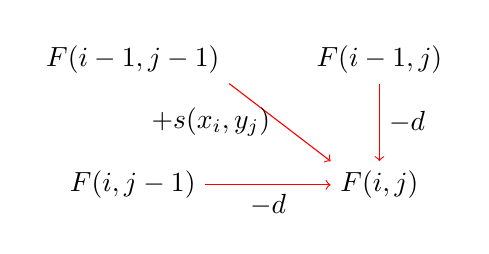
\begin{tikzpicture}
\matrix (m) [matrix of nodes,column sep=10mm,row sep = 10 mm]
{
  $F(i-1,j-1)$ & $ F(i-1,j)$   \\
  $F(i,j-1)$ & $ F(i,j) $  \\
};
% = \max\{F(i-1,j-1) + s(x_i,y_j),F(i-1,j)-d ,F(i,j-1)-d \}
\draw[draw = red, <-] (m-2-2.north west) -- node[left] {$+s(x_i,y_j)$} (m-1-1.south east)  ;
\draw[draw = red, <-] (m-2-2.north) -- node[right] {$-d$} (m-1-2.south) ;
\draw[draw = red, <-] (m-2-2.west) --node[below] {$-d$} (m-2-1.east)  ;
\end{tikzpicture}



Once we have filled out the matrix, we trace back from  $F(n,m)$, following the path that led us here.   That is, the score at the $(n,m)$th position came from one of position  $(n-1,m)$, $(n,m-1)$, or $(n-1,m-1)$ by adding a gap or a match.  We move to whichever position it came from either adding the gap or the match in the process.  In doing so, we build up the alignment from right to left, eventually arriving at $F(0,0)$ at which point we can reverse the alignment to get the full 

Our method is thus based on three things: a recurrence relation, tabular computing and then traceback.  These methods  turn an what is naively an exponential algorithm into a quadratic algorithm ($O(nm)$).

%\begin{tabularx}{0.7\textwidth}{r|X|X|X|X|X|X|}
%\multicolumn{1}{c}{} & \multicolumn{1}{c}{} & \multicolumn{1}{c}{A} & \multicolumn{1}{c}{G} & \multicolumn{1}{c}{T} & \multicolumn{1}{c}{T} & \multicolumn{1}{c}{A}\tabularnewline
%\cline{2-7} 
% &  &&&&& \\ 
%\cline{2-7} 
%A &&&&&& \\ 
%\cline{2-7} 
%T &&&&&& \\ 
%\cline{2-7} 
%A &&&&&& \\ 
%\cline{2-7} 
%\end{tabularx}
%
%\begin{tabularx}{0.7\textwidth}{c|X|X|X|X|X|X|}
%\multicolumn{1}{c}{} & \multicolumn{1}{c}{} & \multicolumn{1}{c}{A} & \multicolumn{1}{c}{G} & \multicolumn{1}{c}{T} & \multicolumn{1}{c}{T} & \multicolumn{1}{c}{A}\tabularnewline
%\cline{2-7} 
% & 0 & $\leftarrow$ -2 &-$\leftarrow$4 & $\leftarrow$-6 &$\leftarrow$-8 &$\leftarrow$-10  \\ 
%\cline{2-7} 
%A &$\uparrow$-2&2&0&-2&-4&-6 \\ 
%\cline{2-7} 
%T &$\uparrow$-4&0&0&2&0&-2 \\ 
%\cline{2-7} 
%A &$\uparrow$ -6&-2&-1&0&0&2 \\ 
%\cline{2-7} 
%\end{tabularx}

{\bf Example:} Align {\tt x = ATA} and {\tt y = AGTTA } with the following scores: the purines  are A and G, while the pyrimidines are  C and T.  Let $s(a,b) = 2$ if $a = b$, 1 if $a$ is purine and $b$ is a purine or $a$ is a pyrimidine and  $b$ is a pyrimidine, and -2 if $a$ is a purine and $b$ is a pyrimidine or vice versa.  Let the gap score be $d = -2$.

{\bf Solution:}
Filling out the matrix and drawing arrows to show where each entry is derived from we get the following:

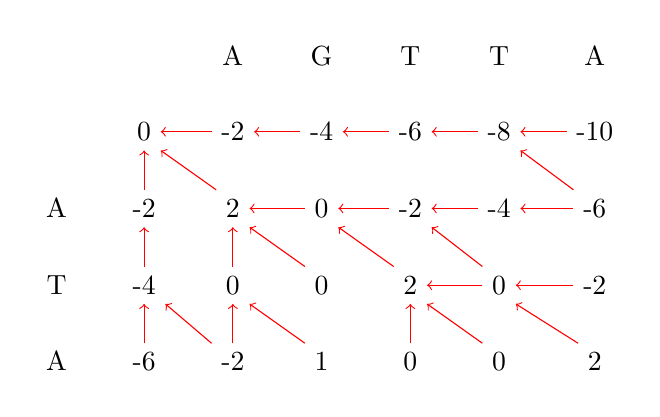
\begin{tikzpicture}
\matrix (m) [matrix of nodes,column sep=6mm,row sep = 5 mm]
{
 &  & A & G & T & T & A  \\
  &0&-2&-4&-6&-8& -10 \\
 A &-2&2&0&-2&-4&-6 \\
 T &-4&0&0&2&0&-2 \\
 A &-6&-2&1&0&0&2 \\
};
\draw[draw = red, ->] (m-3-3.north west) -- (m-2-2.south east);
\draw[draw = red, ->] (m-3-4.west) -- (m-3-3.east);
\draw[draw = red, ->] (m-3-5.west) -- (m-3-4.east);
\draw[draw = red, ->] (m-3-6.west) -- (m-3-5.east);
\draw[draw = red, ->] (m-3-7.west) -- (m-3-6.east);
\draw[draw = red, ->] (m-3-7.north west) -- (m-2-6.south east);
\draw[draw = red, ->] (m-4-3.north) -- (m-3-3.south);
\draw[draw = red, ->] (m-4-4.north west) -- (m-3-3.south east);
\draw[draw = red, ->] (m-4-5.north west) -- (m-3-4.south east);
\draw[draw = red, ->] (m-4-6.north west) -- (m-3-5.south east);
\draw[draw = red, ->] (m-4-6.west) -- (m-4-5.east);
\draw[draw = red, ->] (m-4-7.west) -- (m-4-6.east);
\draw[draw = red, ->] (m-5-3.north west) -- (m-4-2.south east);
\draw[draw = red, ->] (m-5-3.north) -- (m-4-3.south);
\draw[draw = red, ->] (m-5-4.north west) -- (m-4-3.south east);
\draw[draw = red, ->] (m-5-5.north) -- (m-4-5.south);
\draw[draw = red, ->] (m-5-6.north west) -- (m-4-5.south east);
\draw[draw = red, ->] (m-5-7.north west) -- (m-4-6.south east);
\foreach \x/\y in {3/2,4/3,5/4,6/5,7/6}{
\draw[draw = red, ->] (m-2-\x.west) -- (m-2-\y.east);};
\foreach \x/\y in {3/2,4/3,5/4}{
\draw[draw = red, ->] (m-\x-2.north) -- (m-\y-2.south);};
\end{tikzpicture}

The score of the best alignment is given in the bottom right: $F(3,5) = 2$.  To find the alignment with the best score, we traceback from this point.  At $F(2,4)$ there are two choices that produce the same score.  One alignment, found by following the arrow from $F(2,4)$ to  $F(1,3)$ is
\[\begin{array}{ccccc}
A & - & - & T & A \\
A & G & T & T & A
\end{array}\]
while the other is obtained by following the arrow from $F(2,4)$ to  $F(2,3)$ and looks like
\[\begin{array}{ccccc}
A & - & T & - & A \\
A & G & T & T & A
\end{array}\]
 \sqend
% See slides from the lecture and try the applet availalbe in the online notes at \url{ http://www.fos.auckland.ac.nz/~biosci742/3_2.html}.



\subsection{Elements of an alignment algorithm}



We emphasise that these dynamic programming algorithms for sequence alignment are based on following elements:
\begin{itemize}
\item a recurrence relation for the quantity we are trying to optimise, including specification of the boundary conditions,
\item  tabular computing to efficiently calculate the recurrence, and
\item traceback (includes specifying rules for where to start and stop the traceback).
\end{itemize}

By altering the recurrence relation, the boundary conditions or the traceback, we will find different types of ``best'' alignment. Local alignment is  the most common form and is defined below.  


\subsection{Local Alignment: Smith Waterman algorithm}

The Needleman-Wunsch algorithm  looks only at completely aligning two sequences. More commonly, we want to find the best alignment for some subsequence of two sequences. This is the local alignment problem. 

The resulting algorithm that solves this problem is very similar to the one that solve the  global alignment problem.  We derive it as follows.  Redefine $F(i,j)$ to be the score of the best suffix alignment of $x_1 x_2 \ldots x_i$ and $y_1 y_2 \ldots y_j$, where a {\em suffix alignment} is any alignment of $x_s x_{s+1} \ldots x_i$ and $y_r y_{r+1} \ldots y_i$ for some $ 1 \leq s \leq i$ and $1 \leq r \leq j$.  Note that this suffix alignment could be the empty alignment with score 0.

We thus get the recursion 
\[ F_{i,j}= \max 
\begin{cases}
0\\
F(i-1,j-1)+s(x_i,y_i), \\
F(i-1,j)-d, \\
F(i,j-1)-d.
\end{cases} \]
So instead of a letting a score for an alignment to go negative, we start a new alignment. To find the best subsequence alignment, then, we simply look for the best score and trace it back until we hit a 0. Note than we can now start and finish anywhere in the matrix.

{\bf Example:} Find the best local alignment using the score matrix and sequences given in the previous example: {\tt x = ATA} and {\tt y = AGTTA }

{\bf Solution:}  Fill out the matrix, drawing an arrow when a cell has a predecessor to get the following.

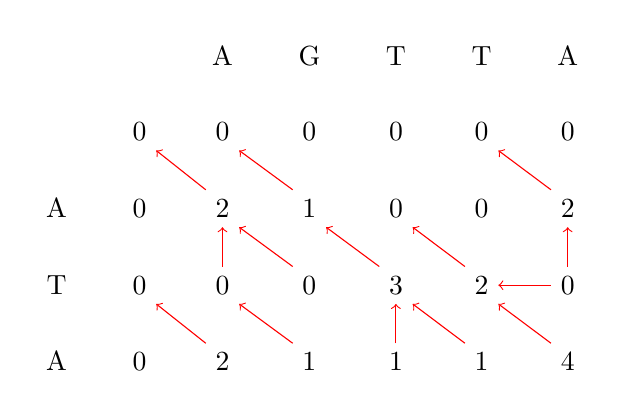
\begin{tikzpicture}
\matrix (m) [matrix of nodes,column sep=6mm,row sep = 5 mm]
{
 &  & A & G & T & T & A  \\
  &0&0&0&0&0& 0 \\
 A &0&2&1&0&0&2 \\
 T &0&0&0&3&2&0 \\
 A &0&2&1&1&1&4 \\
};
\draw[draw = red, ->] (m-3-3.north west) -- (m-2-2.south east);
\draw[draw = red, ->] (m-3-4.north west) -- (m-2-3.south east);
\draw[draw = red, ->] (m-3-7.north west) -- (m-2-6.south east);
\draw[draw = red, ->] (m-4-3.north) -- (m-3-3.south);
\draw[draw = red, ->] (m-4-4.north west) -- (m-3-3.south east);
\draw[draw = red, ->] (m-4-5.north west) -- (m-3-4.south east);
\draw[draw = red, ->] (m-4-6.north west) -- (m-3-5.south east);
\draw[draw = red, ->] (m-4-7.north) -- (m-3-7.south);
\draw[draw = red, ->] (m-4-7.west) -- (m-4-6.east);
\draw[draw = red, ->] (m-5-3.north west) -- (m-4-2.south east);
\draw[draw = red, ->] (m-5-4.north west) -- (m-4-3.south east);
\draw[draw = red, ->] (m-5-6.north west) -- (m-4-5.south east);
\draw[draw = red, ->] (m-5-7.north west) -- (m-4-6.south east);
\draw[draw = red, ->] (m-5-5.north) -- (m-4-5.south);
\end{tikzpicture}

The score of the highest scoring local alignment is the largest entry in this matrix.  We find this at $(5,3)$ where $F(5,3) = 4$.  The sub alignment is found by tracing back from that cell and stopping at the first cell with no predecessor (or at the first 0 encountered).  This produces the local alignment 

\( \begin{array}{cc}
T & A \\
T & A
\end{array}\)
 \sqend



%\subsection{Variations on a theme}




%\subsubsection{Repeated matches}
%
%In the repeated matches problem, we suppose there is a repeated domain or motif (described by sequence $y$) in a sequence $x$ and we wish to find copies of these repeats. We assume that the score for a match needs to be at least $T > 0$ to ensure spurious matches will not be included. The boundary condition is $F (0, 0) = 0$ and the recurrence is
%\[ F_{i,0}= \max 
%\begin{cases}
%F(i-1,0),\\
%F(i-1,j)-T, \, j = 1,\ldots,m;
%\end{cases} \]
%
%\[ F_{i,j}= \max 
%\begin{cases}
%F(i,0),\\
%F(i-1,j-1)+s(x_i,y_i), \\
%F(i-1,j)-d, \\
%F(i,j-1)-d.
%\end{cases} \]
%Start the traceback at the additional cell, $F (n + 1, 0)$ (calculated using the rule for $F (i, 0)$).

\subsubsection{Overlap matches}

As an example of how easy it is to establish different types of alignment algorithm we consider a special type of alignment known as an overlap alignment.  


When we expect one sequence to completely contain another or that they overlap, we want a global type alignment that does not penalize the unmatched overhanging ends. The boundary conditions are $F (i, 0) = F (0, j) = 0$ for all $i, j$, the recurrence relation is just the global recurrence and we start the traceback at the position on the right  or top boundary the maximum score taken over all scores on those boundaries is achieved, $F (i, m)$ or $F (n, j)$. The traceback stops when either the left or top border  is reached, $F (i, 0)$ or $F (0, j)$.


\subsection{Pairwise alignment with non-linear gap penalties }

In our pairwise alignment discussion, we only considered linear gap penalties.  As we noted earlier, linear penalties are a poor model for biological sequence data where we expect gaps (that is, insertions or deletions) to be quite rare but if there is a gap it may be multiple  bases in length.  Thus, an affine penalty, which penalises the start of the gap more heavily than any extension to the gap is favoured.

For an arbitrary  gap penalty,  $\gamma(k)$, we can continue to use a similar dynamic programming approach as before, but a direct adoption of that approach results in a much slower algorithm. Let's investigate: With a general gap penalty, $\gamma(k)$, the recurrence relation becomes 
\[ F_{i,j}= \max 
\begin{cases}
F(i-1,j-1)+s(x_i,y_j), \\
F(k,j) + \gamma(i - k), \hspace{1cm} k = 0,\ldots,i-1,  \\
F(i,k) + \gamma(j-k),\hspace{1cm} k = 0,\ldots,j-1  .
\end{cases} \]
This means that to calculate the value of each cell in the matrix $F(i,j)$ we need to consider $i+j+1$ other cells --- the $i$ previous cells in the row, the $j$ previous cells in the column, and the one adjacent diagonal cell --- rather than the 3 as we had with the linear gap penalty (see Figure below).  This results in a $O(n^3)$ algorithm rather than a $O(n^2)$

To calculate an unknown cell of $F$, the scores for gaps of all possible lengths need to be calculated meaning that a calculation for each previous cell in the row and column needs to be made: \\
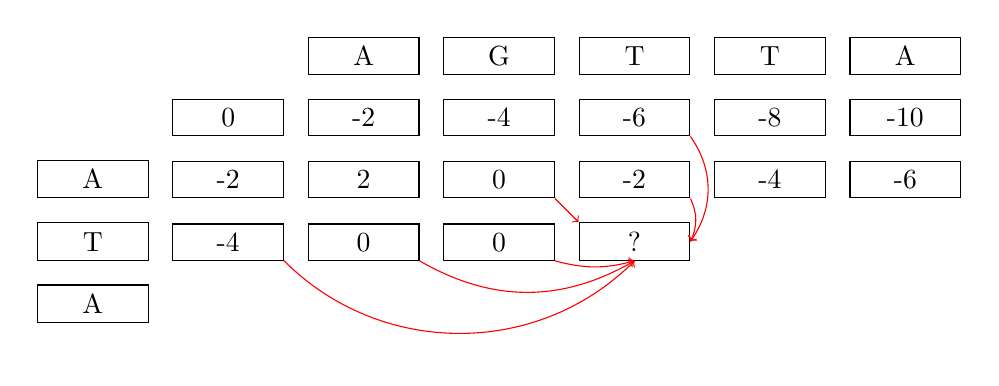
\begin{tikzpicture}
\matrix (m) [matrix of nodes,column sep=3mm,row sep = 3 mm, style={nodes={rectangle,draw,minimum width=4em}}]
{
 &  & A & G & T & T & A  \\
  &0&-2&-4&-6&-8& -10 \\
 A &-2&2&0&-2&-4&-6 \\
 T &-4&0&0&? & & \\
 A & & & & & &   \\
};
\draw[draw = red, <-] (m-4-5.south) to [bend left = 15] (m-4-4.south east);
\draw[draw = red, <-] (m-4-5.south) to [bend left = 30] (m-4-3.south east);
\draw[draw = red, <-] (m-4-5.south) to [bend left = 45] (m-4-2.south east);
\draw[draw = red, <-] (m-4-5.east) to [bend right = 25] (m-3-5.south east);
\draw[draw = red, <-] (m-4-5.east) to [bend right = 35] (m-2-5.south east);
\draw[draw = red, <-] (m-4-5.north west) to (m-3-4.south east);
\end{tikzpicture}


\subsection{Alignment with affine gap scores}


In the case of an affine gap score (which has the form $\gamma(k) = -d - (k-1)e$\,) it turns out that we can, once again, construct a $O(n^2)$ dynamic programming algorithm to solve the alignment problem.
The only difficulty is that we now have to keep track of 3 possible states corresponding to 3 cases:
\begin{enumerate}
\item Let $M(i,j)$ be the best score of the alignment up to $(i,j)$ given that $x_i$ is aligned to $y_j$. This case looks like\\
{\tt A C C $\mathtt{x_i}$ \\
A C G $\mathtt{y_j}$}
\item Let $I_x(i,j)$ be the best score of the alignment up to $(i,j)$ given that $x_i$ is aligned to a gap. This case looks like\\
{\tt A C C $\mathtt{x_i}$ \\
  G $\mathtt{y_j}$   - -}
\item Let $I_y(i,j)$ be the best score of the alignment up to $(i,j)$ given that $y_j$ is aligned to a gap. This case looks like\\
{\tt  C C $\mathtt{x_i}$  - \\ 
A C G  $\mathtt{y_j}$ }
\end{enumerate}
Given those definitions, and assuming that a gap cannot directly follow an insertion (that is, we can't go directly from $I_x$ to $I_y$ or vice versa), we have the following recurrence relations:
\[ M(i,j)= \max 
\begin{cases}
M(i-1,j-1)+s(x_i,y_j), \\
I_x(i-1,j-1)+s(x_i,y_j), \\
I_y(i-1,j-1)+s(x_i,y_j); 
\end{cases} \]
\[ I_x(i,j)= \max 
\begin{cases}
M(i-1,j)-d, \\
I_x(i-1,j)-e; 
\end{cases} \mbox{and}, \]
\[ I_y(i,j)= \max 
\begin{cases}
M(i,j-1)-d, \\
I_y(i,j-1)-e. 
\end{cases} \]
It should be clear that we can calculate this recursion efficiently using tabular computation where we have 3 arrays: one for each of $M$, $I_x$ and $I_y$.  We can use a similar back-tracking mechanism to find the best alignment once we have calculated the scores.  

This results in an quadratic time and space algorithm once again but the coefficient of the quadratic term is greater for this algorithm than the linear gap penalty one.  For example, the space requirement here is $3n^2$ while it is only $n^2$ with a linear gap penalty.  

The above recursions can be very neatly represented as a {\em finite state automaton}, or FSA.  

\begin{figure}[ht]
\centering
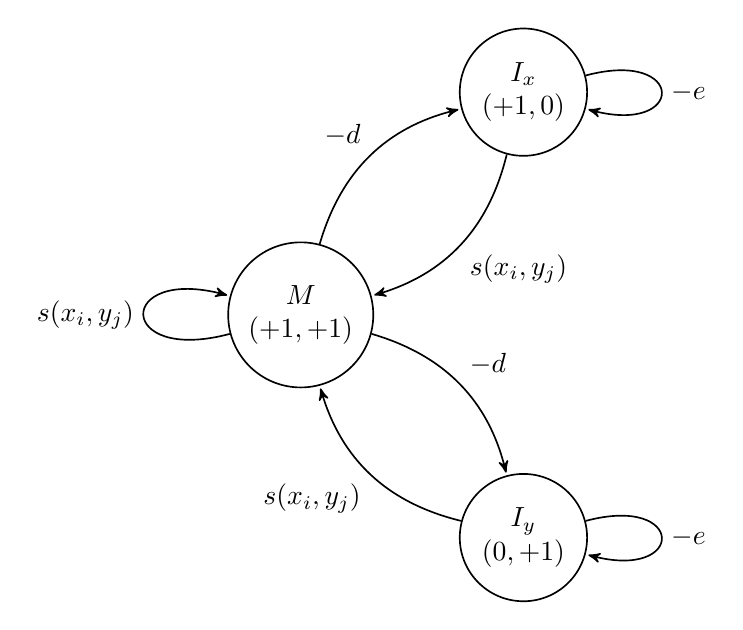
\begin{tikzpicture}[->,>=stealth',shorten >=1pt,auto,node distance=4cm,
                    semithick,every text node part/.style={align=center}]
  \tikzstyle{every state}=[fill=none,draw=black,text=black]

  \node[state] (M)                    {$ M$\\$ (+1,+1)$};
  \node[state]         (Ix) [above right of=M] {$I_x$\\$(+1,0)$};
  \node[state]         (Iy) [below right of=M]       {$I_y$\\$ (0,+1)$};

  \path (M) edge       [bend left]        node {$-d$} (Ix)
          (M) edge [loop left] node {$s(x_i,y_j)$} (M)
          (Ix) edge       [bend left]        node {$s(x_i,y_j)$} (M)
          (Ix) edge [loop right] node {$-e$} (Ix)
          (Iy) edge       [bend left]        node {$s(x_i,y_j)$} (M)
          (Iy) edge [loop right] node {$-e$} (Iy)
          (M) edge [bend left] node {$-d$} (Iy);
 \end{tikzpicture}
\caption{A finite state automaton describing the affine gap alignment recurrence relation. The pairs of numbers below the state names indicate how we  increment the position in sequence $x$ and $y$. }
 \label{fig:fsa}
 \end{figure}
 
 
 In an FSA, each of the three possibilities, match, insertion in $x$ or insertion in $y$, corresponds to a state (drawn as circles).  
 
 The transitions each carry a score, as indicated next to the arrow.
 
 The new value for the state variable at $(i,j)$ is the maximum of the scores corresponding to the transitions coming into the state.  Each transition score is given by is given by the value of the source state at the offsets specified by the $\delta (i,j)$ pair of the target state plus the specified score increment.
 
 An alignment corresponds to a path through the states.
 
 \begin{verbatim}
V  L  S  P  A  D  -  K
H  L  -  -  A  E  S  K

m  m  Ix Ix m  m  Iy m
\end{verbatim}

 
 These automata are known in computer science as Moore machines.
 
 We've already seen one type of FSA: a Markov chain can be represented as a stochastic FSA.  We'll look at another stochastic FSA, the hidden Markov model or HMM, shortly.

%%%\notinexam{
\subsection{Linear space alignment}

If sequences are large, even a quadratic algorithm can be difficult to work with.  We can't improve the speed of the algorithm but we can reduce the amount of memory we need (currently at that is $O(n^2)$ too).

If all we require is the {\em score} of the best alignment, we immediately see that we don't need to keep the whole matrix until the end of the alignment.  In the case of global alignment, the score of the best alignment is given by the entry $F(m,n)$.  To calculate any score in the $i$th row, all we need to know is the $(i-1)$th row, so we only need to keep the a single row of the matrix in memory.  A similar argument can be made for the score of the best local alignment.

If we actually want the best alignment, it turns out that we can still produce a linear space algorithm.  We employ  a {\em divide and conquer} approach.  Suppose we could find a cell, $(i^\ast,j^\ast)$ what we knew to lie on the optimal alignment.  Then we could divide the alignment problem into two halves: from $(0,0)$ to $(i^\ast,j^\ast)$ then from $(i^\ast,j^\ast)$ to $(m,n)$.  In the best case, this reduces the amount of storage space require by 2.  This process can be iterated, so  $(i^{\ast \ast},j^{\ast \ast})$ is found to reduce the space required for the $(0,0)$ to $(i^\ast,j^\ast)$ section and so on.   It turns out that given an $i^\ast$, a suitable $j^\ast$ can be found.   We omit the details here (they are not too difficult) but  details and references are given towards the end of chapter 2 in the Durbin et al book.
%
%
%\newpage
%
%%} % end not in exam

\section{Multiple sequence alignments (MSA)}

In pairwise alignment, we were given two sequences, $x$ and $y$ and wanted to align them by judiciously inserting gaps so that homologous residues were lined up with one another.  

Multiple alignment is similar except now we have $k \geq 3$ sequences to align, so we want to form columns of homologous residues by adding gaps to each sequence.  

Experts can construct multiple alignments by hand by considering a number of factors like secondary and tertiary protein structure, highly conserved regions, patterns of gaps, evolutionary processes etc.    This is, however, subjective, difficult and tedious. 

We want to come up with a method that is probabilistic, automatic and produces alignments that experts are happy with.

A good entry point to understanding the problem of global alignment is the {\tt Phylo} puzzle game at \url{http://phylo.cs.mcgill.ca/} where you work on short multiple alignments by hand. 



%\subsubsection{Resources}
%
%Read chapter 6 of the Durbin et al book.
%
%An online lecture from BioSci742 covers much of this material: \url{http://www.fos.auckland.ac.nz/~biosci742/3_6.html}.  In particular, check out the applet showing how progressive MSA is performed: \url{http://www.fos.auckland.ac.nz/~biosci742/applets/multseqalign.html}.
%
%The Clustal$\Omega$ website: \url{http://www.clustal.org/omega/} and paper: \url{http://www.nature.com/msb/journal/v7/n1/full/msb201175.html}. 

\subsection{Dynamic programming}

It is tempting to try to extend the dynamic programming methods that we used for pairwise alignments to the MSA problem.  It is relatively easy to write down the naive extension of pairwise alignment algorithms to more than 2 sequences. But the naive implementation quickly becomes impossible as the number of sequences and the length of the sequences increases.  

For example, for 2 sequences of length $L$, the Needleman-Wunsch algorithm requires a 2-dimensional array with $L^2$ cells in total to be stored in memory.  The MSA analogue on $n$ sequences  requires storing an $n$-dimensional array containing  $L^n$ cells in total.  Even for short sequences of $L = 100$, we would require memory for $100^5 = 10^{10}$ cells (at 4 bytes per cell, that's about 37 GB).  

Some clever work from Lipman, Altschul and Kececioglu (the first two co-wrote BLAST) managed to reduce the size of the space that needs to be considered.  That is, instead of calculating all $L^n$ cells, they calculate upper and lower bounds on the score of the best MSA and then need only calculate the cells in the $n$-dimensional array that will produce scores lying between these two bounds.   This work allows a few sequences (5-10) of moderate length (300 residues) and not too far diverged to be optimally aligned but even this requires a large computational resource.


\subsection{Progressive alignment}

Finding the optimal MSA is computationally  prohibitive, as discussed in the previous Section.  Typically, we resort to finding a good-enough alignment using heuristic techniques.  The most widely used heuristic is progressive alignment.  

Progressive alignment involves a series of successive pairwise alignments.  At it's most basic, an initial pair of sequences are chosen and aligned, a third is chosen and aligned to the first two and so on until all sequences are included in the MSA.  Other methods also allow the aligning of two alignments to each other.  For example, if there are 4 sequences, two pairs may be aligned first then the two alignments aligned to complete the MSA. 

These methods require that we can: decide on an order in which to align the sequences, align two sequences together, align a sequences to a MSA and align two MSAs together.  

The typical way to decide on the order in which to align the sequences is to build a guide tree, using a clustering methods such as UPGMA, and align sequences in the order that nodes occur from the leaves to the root of the tree. 
  
\subsection{Building trees with distances and UPGMA} \label{sec:UPGMA}

%The fastest ways of constructing trees rely on defining a distance between sequences.  There are numerous ways of defining distances between sequences.  The simplest, for an aligned pair of sequences $x$ and $y$ of length $L$ is to count the number of positions where they differ, $D_{xy}$ say, and define the distance to be  $f_{xy} = D_{xy}/L$, that is, the fraction of sites at which they differ.  This method works well for  related sequences where $f$ is expected to be small, but doesn't grow as much as we would like as sequences become less and less related since even unrelated sequences share many bases in common due to chance.

%The Jukes-Cantor distance is based on the simplest model of sequence evolution where mutations between all four bases are equally likely.  The distance is defined by $d_{xy} = -\frac34 \log {(1- \frac{4f_{xy}}3)}$. The Jukes-Cantor distance tends to infinity as the fraction of shared residues tends to the expected background level for unrelated sequences.

UPGMA is a method of building trees based on distances: we are given a set of objects, and for each pair of objects we have some measure of the distance between them.  

UPGMA stands for unweighted pair group method using arithmetic averages and is a simple method with an ugly name.  The idea can be thought of as a clustering algorithm where we start with all individual sequences  and start clustering them together, building the tree up from the leaves to the root.  The height of the internal nodes (or, equivalently, the edge lengths) is determined by the distances between the two clusters being joined.  

For two sequences, $x$ and $y$, we assume we have a method of defining the distance $d_{xy}$.  We define the distance between two clusters of sequences, $C_i$ and $C_j$ as the average distance between all pairs between clusters:
\[ d_{ij} = \frac1{|C_i| |C_j|}\sum_{x \in C_i,y \in C_j} d_{xy}\]
where $|C|$ is the number of sequences in cluster $C$.

We define the algorithm as follows:
\begin{description}
\item[Initialise]  Assign each sequence $i$ to it's own cluster $C_i$. Assign a leaf node to each cluster and give it height 0.
\item[Repeat until there only one cluster remains]  Find clusters $C_i$ and $C_j$ such that $d_{ij}$ is minimal (choose randomly between equidistant candidates). 

Join $i$ and $j$ to make the new cluster $C_k = C_i \cup C_j$.

Define a node $k$ in the tree placed at height $d_{ij}/2$ with child nodes $i$ and $j$.

Update the distance matrix.
\end{description}

This procedure results in a well-defined tree (we need to check that all node heights are above the heights of the their children).  The algorithm is quadratic ($O(n^2)$) in the number of sequences.


{\bf Example:} Given 4 sequences, $A,B,C$ and $D$, which have the pairwise distances given by the distance matrix $d$ below, construct the UPGMA tree.
\[ d= \begin{array}{ccccc}
& A& B&C&D \\
A &-&4 & 8 & 8 \\
B & & - & 8 & 8 \\
C & & & - & 6 \\
D &&&& -
\end{array}
\]
{\bf Solution:}  Start by assigning leaf nodes to each of the sequences with height 0:

\tikzset{vertex/.style = {circle, draw, fill=black!50,inner sep=0pt, minimum width=4pt}}
\begin{tikzpicture}[thick,scale=1]
\node at (0,.2) {};
    \node [vertex,label = below:$A$] at (0,0) (A) {} ;
    \node [vertex,label = below:$B$] at (1,0) (B) {} ;
    \node [vertex,label = below:$C$] at (2,0) (C) {} ;
    \node [vertex,label = below:$D$] at (3,0) (D) {} ;  
        \node at (4,0)  {0} ;

\end{tikzpicture}

Now choose the pair of clusters that are closest to each other according to the distance matrix $d$.  This is the pair $(A,B)$ with distance $d(A,B) = 4$. Join the cluster $E = A \cup B = \{A,B\}$ which has height $d(A,B)/2 = 2$.

\begin{tikzpicture}[thick,scale=1]
    \node [vertex,label = below:$A$] at (0,0) (A) {} ;
    \node [vertex,label = below:$B$] at (1,0) (B) {} ;
    \node [vertex,label = below:$C$] at (2,0) (C) {} ;
    \node [vertex,label = below:$D$] at (3,0) (D) {} ;
    \node [vertex,label = left:$E$] at (0.5,2) (E) {} ;
    \node at (4,0)  {0} ;
    \node at (4,1)  {1} ;
    \node at (4,2)  {2} ;
         
     \path (A) edge  (E);
     \path (B) edge  (E);

\end{tikzpicture}

The distance matrix is by calculating $d(E,C)$ and $d(E,D)$.  $d(E,C) =  \frac1{2\cdot 1}(d(A,C) + d(B,C)) = \frac 1 2 (8+8) = 8$ and similarly for $d(E,D)$.
\[ \begin{array}{cccc}
& E&C&D \\
E & - & 8 & 8 \\
C &  & - & 6 \\
D &&& -
\end{array}
\]
Now form the cluster $F = \{C,D\}$ and place the node at $d(C,D)/2 = 3$.

\begin{tikzpicture}[thick,scale=1]
    \node [vertex,label = below:$A$] at (0,0) (A) {} ;
    \node [vertex,label = below:$B$] at (1,0) (B) {} ;
    \node [vertex,label = below:$C$] at (2,0) (C) {} ;
    \node [vertex,label = below:$D$] at (3,0) (D) {} ;
    \node [vertex,label = left:$E$] at (0.5,2) (E) {} ;
    \node [vertex,label = left:$F$] at (2.5,3) (F) {} ;
    \node at (4,0)  {0} ;
    \node at (4,1)  {1} ;
    \node at (4,2)  {2} ;
    \node at (4,3)  {3} ;
         
     \path (A) edge  (E);
     \path (B) edge  (E);
     \path (C) edge  (F);
     \path (D) edge  (F);

\end{tikzpicture}

The distance matrix is now the single distance between the remaining clusters: $d(E,F) = \frac 1 {2\cdot 2} (d(A,C)+d(A,D) + d(B,C)+d(B,D) ) = \frac 1 4 (8+8+8+8) = 8$. So make the last node $G = \{E,F\}$ and place it at height $8/2 = 4$.  The UPGMA tree is thus

\begin{tikzpicture}[thick,scale=1]
    \node [vertex,label = below:$A$] at (0,0) (A) {} ;
    \node [vertex,label = below:$B$] at (1,0) (B) {} ;
    \node [vertex,label = below:$C$] at (2,0) (C) {} ;
    \node [vertex,label = below:$D$] at (3,0) (D) {} ;
    \node [vertex,label = left:$E$] at (0.5,2) (E) {} ;
    \node [vertex,label = left:$F$] at (2.5,3) (F) {} ;
    \node [vertex,label = left:$G$] at (1.5,4) (G) {} ;
    \node at (4,0)  {0} ;
    \node at (4,1)  {1} ;
    \node at (4,2)  {2} ;
    \node at (4,3)  {3} ;
    \node at (4,4)  {4} ;
         
     \path (A) edge  (E);
     \path (B) edge  (E);
     \path (C) edge  (F);
     \path (D) edge  (F);
     \path (E) edge  (G);
     \path (F) edge  (G);

\end{tikzpicture}
\sqend


%Another commonly used distance method is neighbor-joining.  It is also relatively simple but we omit it here.  See section 7.3 of Durbin, Eddy et al.



\subsection{Feng-Doolittle progressive alignment}

The Feng-Doolittle algorithm (1987) takes the approach described above.  The steps for aligning $n$ sequences are as follows.  
\begin{enumerate}
\item Calculate the $n(n-1)/2$ distances between all sequences pairs.  The distances are found by aligning each pair and recording a normalized score.  The score used is \[D = -\log S_{eff}  = -\log \frac{S_{obs} - S_{rand}}{S_{max} - S_{rand}}\] where $S_{obs}$ is the score from the pairwise alignment, $S_{max}$ is the average of scores obtained by aligning each sequences of the pair to itself and $S_{rand}$ is the expected score for an alignment of the pair when the residues are randomly shuffled. The effective score $S_{eff}$ can thus be
viewed as a normalised percentage similarity which  roughly decays exponentially towards zero with increasing evolutionary distance.  Thus, we take $ -\log$ to
make the score decay approximately linearly with evolutionary distance.
\item Build a guide tree based on the recorded scores (we use UPGMA).
\item Build the alignment in the order that nodes were added to the tree. 
\end{enumerate}
A pair of sequences is aligned in the normal way. A sequence is aligned to an MSA by aligning it to each sequence in the MSA and choosing the highest scoring alignment.  Two alignments  are aligned to each other by aligning all pairs of sequences between the two groups and choosing the best alignment.  

After a sequence or group of sequences is added to an alignment, the introduced gap characters are replaced with a neutral $X$ character which can be aligned to any other character (gap or residue) with no cost. Crucially, there is no penalty for aligning a gap to an $X$  which tends to make gaps align with each other, giving us the characteristic pattern we see in multiple alignments of gaps clustered in columns.

Once the initial MSA has been found, we can use further heuristics to improve it and lessen any effect  of the order in which sequences were added.  For example, we can choose a sequence uniformly at random, remove it from the MSA and then realign it to the the MSA.  This process can be iterated until the MSA becomes stable, that is, no or very few changes occur when a sequence is removed and re-aligned  

\newpage
 
\section{Hidden Markov Models}


In Markov models, we directly observe the state of the process (for example, in a random walk, the state is completely described by the position of the random walker). We can easily imagine a system where we don't directly observe the state but observe some outcome which depends on the state. Call the observed outcomes {\em symbols}.  We thus make a distinction between the {\bf sequence of states} and the {\bf sequence of symbols}.  We formally model these systems as hidden Markov models (HMMs).

%Let's look at an example:

{\bf Example:} Weather.  Suppose we live in a place that gets winds  either from the  south or north.  On days the wind is from the south, it is rainy and cold 75\% of the days, and warm and sunny the other 25\% of the days.  When the wind is from the north, is is   rainy and cold 20\% of days, and warm and sunny 80\% of the days.    If it is northerly today, it will be northerly tomorrow with probability 0.7.  If it is southerly today it will be south with prob. 0.6. \sqend


\tikzstyle{state}=[shape=circle,draw=blue!50,fill=blue!20]
\tikzstyle{observation}=[shape=rectangle,draw=orange!50,fill=orange!20]
\tikzstyle{lightedge}=[<-,dotted]
\tikzstyle{mainstate}=[state,thick]
\tikzstyle{mainedge}=[<-,thick]
 
\begin{figure}[htbp]
\begin{center}
\begin{tikzpicture}[]
% states
\node[state] (N) at (1,3) {$N$}
    edge [loop above] node[above] {$0.7$} ();
\node[state] (S) at (3,3) {$S$}
    edge [<-,bend right=45] node[auto,swap] {$0.3$} (N)
    edge [->,bend left=45] node[auto,swap] {$0.4$} (N)
    edge [loop above] node[above] {$0.6$} ();
% observations
\node[observation] (y1) at (0,0) {Rain ($R$)}
    edge [lightedge] node[left] {0.2} (N)
    edge [lightedge] node[left] {0.75} (S);
\node[observation] (y2) at (4,0) {Sun ($U$)}
    edge [lightedge]  node[right] {0.8} (N)
    edge [lightedge]  node[right] {0.25} (S);
\end{tikzpicture}
\end{center}
\caption{The chance of Sunny or Rainy weather on a day is determined by the wind direction.  When it is Northerly, Sun is more likely, when it is Southerly, Rain is more likely. }
\end{figure}





% In the Weather case, the underlying state is the wind direction and what is being produced is either warm and sunny or cold and rainy.  In the casino case, the state is the die being used, the observations are what numbers are being rolled.  In the Sequence case, the state is whether or not we are in a CpG island but what is produced in all states are a mix of As, Cs, Gs, and Ts.  We thus make a distinction between the {\bf sequence of states} and the {\bf sequence of symbols}.

The idea in the HMM is that we only observe the sequence of symbols but to understand what is going on, we need to know what the underlying state is.


{\bf Example cont.:} A state sequence for the weather example might be $NNNSSNS$ while the emissions sequence looks like (using $R$ for rain and $U$ for sun)  $UUUURUR$. We might observe the weather (rainy or sunny) and wonder what is causing the patterns we see.  The pattern is best understood by knowing the sequence of states (direction of wind). \sqend

\subsubsection*{Notation for HMMs}

The $i$th state of the state sequence is $\pi_i$ and transitions (of the states) is given by $a_{kl} = P(\pi_i  = l | \pi_{i-1} = k)$.  We use $b$'s to represent the symbols so we get a new set of parameters called  emission probabilities, $e_{\pi}(b) = P(x_i = b | \pi_i = \pi)$ is the prob of emitting symbol $b$ given that we are in state $\pi$.

{\bf Example cont.:} In the weather example $a_{NN} = 0.7$, $a_{NS} = 0.3$, $a_{SS} = 0.6$ and $a_{NS} = 0.4$.  The emission probabilities are $e_N(R) = 0.2$, $e_N(U) = 0.8$, $e_S(R) = 0.75$ and $e_S(U) = 0.25$. \sqend

\begin{figure}[htbp]
\begin{center}
\begin{tikzpicture}[]
% states
\node[state] (N) at (1,3) {$N$}
    edge [loop left] node[left] {$a_{NN} = 0.7$} ();
\node[state] (S) at (3,3) {$S$}
    edge [<-,bend right=45] node[auto,swap] {$a_{NS} = 0.3$} (N)
    edge [->,bend left=45] node[below,swap] {$a_{SN} = 0.4$} (N)
    edge [loop right] node[right] {$a_{SS} = 0.6$} ();
% observations
\node[observation] (y1) at (0,0) {Rain ($R$)}
    edge [lightedge] node[left] {$e_N(R) = 0.2$} (N)
    edge [lightedge] node {$0.75$} (S);
\node[observation] (y2) at (4,0) {Sun ($U$)}
    edge [lightedge]  node[right] {$0.8$} (N)
    edge [lightedge]  node[right] {$e_S(U) =0.25$} (S);
\end{tikzpicture}
\end{center}
\caption{The chance of Sunny or Rainy weather on a day is determined by the wind direction.  When it is Northerly, Sun is more likely, when it is Southerly, Rain is more likely. }
\end{figure}


{\bf Example:} Cheating Casino.  A casino tips things in its favour at a dice table by occasionally switching from a fair die to a loaded one.  The loaded die produces a 6 50\% of the time, and each of 1-5 just 10\% of the time.  Call the fair die $F$ and the loaded die $L$.  We have transitions $a_{FL} = 0.05$ and $a_{LF} = 0.1$.  $a_{FF} = 1 - a_{FL}$ and $a_{LL} = 1 - a_{LF}$.  Emissions are $e_F(b) = 1/6$ for $b = 1,\ldots,6$ while $e_L(b) = 1/10$ for $b = 1,\ldots,5$ and $e_L(6 ) = 0.5$.

\begin{figure}[htbp]
\begin{center}
\begin{tikzpicture}[]
% states
\node[state] (F) at (1,3) {$F$}
    edge [loop left] node[left] {$a_{FF} = 0.95$} ();
\node[state] (L) at (4,3) {$L$}
    edge [<-,bend right=45] node[auto,swap] {$a_{FL} = 0.05$} (F)
    edge [->,bend left=45] node[above,swap] {$a_{LF} = 0.1$} (F)
    edge [loop right] node[right] {$a_{LL} = 0.9$} ();
% observations
\node[observation] (y1) at (0,0) {1}
    edge [lightedge] (L)
    edge [lightedge]  node[left] {$e_F(x) = 1/6$} (F);
\node[observation] (y2) at (1,0) {2}
    edge [lightedge] (L)
    edge [lightedge] (F);
\node[observation] (y3) at (2,0) {3}
    edge [lightedge] (L)
    edge [lightedge] (F);
\node[observation] (y4) at (3,0) {4}
    edge [lightedge] (L)
    edge [lightedge] (F);
\node[observation] (y5) at (4,0) {5}
    edge [lightedge] (L)
    edge [lightedge] (F);
\node[observation] (y6) at (5,0) {6}
    edge [lightedge] node[right] {$e_L(6) = 1/2, \mbox{ else }e_L(x) =  1/10 $} (L)
    edge [lightedge] (F);
%\node[observation] (y2) at (4,0) {Sun ($U$)}
%    edge [lightedge]  node[right] {$e_N(U) =0.8$} (N)
%    edge [lightedge]  node[right] {$e_S(U) =0.25$} (S);
\end{tikzpicture}
\end{center}
\caption{}
\end{figure}


A run of the chain might look like:\\ {\tt F F F F L F F F L L L L L L L L F F F F F F F F F F F F F F L L L L F F F F L L L L L L F F F F F F F F}\\
producing  rolls  \\
{\tt 2 5 1 6 6 2 4 2 4 5 6 6 3 6 2 4 2 2 3 4 6 3 6 5 3 4 5 2 3 5 1 6 6 6 6 2 4 6 6 2 6 6 6 6 6 1 5 1 6 4 1 2. } \sqend

Think of HMMs as a generative process where the first state $\pi_1$ is chosen according to probability $a_{0i}$.  From that state, a symbol is emitted according to the probabilities $e_{\pi_1}$.  State 2 is then chosen according to transition probs $a_{\pi_1  i}$ which emits a symbol and so on. 

 The joint probability of states and symbols is then, 
 \[ P(x,\pi) = a_{0 \pi_1} \prod_{i = 1}^L e_{\pi_i}(x_i)a_{\pi_i \pi_{i+1}} \]



\subsection{The Viterbi algorithm for finding the most probable state path}

Multiple underlying states could produce the same path.  Clearly, though, some states are more likely than others given the emissions.  If we see lots of very good weather, for example, we may guess that northerlies are predominating in our city.  If we see long strings of 6s, we might guess that the casino has switched to the loaded die, while sequences of apparently evenly distributed throws suggest a fair die is being used.  

If we want to work with just one state path, it can be argued that the state path with the highest probability is the one to choose.  Let
\[ \pi^* = \argmax_{\pi} P(x,\pi). \]
We can find $\pi^*$ using a recursive algorithm due to Andrew Viterbi (an  Jewish Italian refugee from the fascists who grew up in the USA, wrote this algorithm while at MIT and then started Qualcomm, a now huge technology company).   

Let $v_k(i)$ be the probability of the most probable state path ending in state $k$ at observation $i$ (that is, considering only the first $i$ observations).  Suppose  $v_k(i)$ is known for all states $k$.  Then the next probability $v_l(i+1)$ can be calculated for observation $x_{i+1}$ as 
\[v_l(i+1) = e_l(x_{i+1}) \max_k (v_k(i)a_{kl}).\]

If we insist that all sequences start in a begin state called 0, we have $v_0(0) = 1$ and we can use a backtracking procedure like we saw in the pairwise alignment algorithm to find the most probable path.

The Viterbi algorithm thus proceeds as follows:
\begin{description}
\item[Initialisation $i = 0$:] $v_0(0) = 1$, $v_k(0) = 0$ for $k>0$.
\item[Recursion $i = 1,\ldots,L$:] $v_l(i) = e_l(x_i) \max_k(v_k(i-1)a_{kl})$. \\ $Pointer_i(l) = \argmax_k(v_k(i-1)a_{kl})$
\item[Termination:] $P(x,\pi^*) = \max_k (v_k(L)a_{k0})$. $ \pi^*_L = \argmax_k(v_k(L)a_{k0})$.
\item[Traceback $i = L,\ldots,1$:] $\pi_{i-1}^* = Pointer_i(\pi_i^*)$.
\end{description}
Here we assume an end state is modeled, as $a_{k0}$.  If the end is not modeled, this term disappears.


Even the most probable path typically has a very low likelihood, so it is important to work in log units.  The recursion in log units is \[ V_l(i+1) = \log (e_l(x_{i+1})) + \max_k (V_k(i) + \log(a_{kl}))\]
where $V_k(i) = \log(v_k(i))$.



{\bf Example:}   In the human genome, the dinucleotide (that is, two base pairs next to each other in the sequence) CG, written CpG to distinguish it from the nucleotide pair C-G, is subject to methylation.  Methylation changes the G to a T.  That means we see the CpG dinucleotide less frequently than we would expect by considering the individual frequencies of C and G.  In some functional regions of the genome, such as promoter and start regions of genes,  methylation is suppressed and CpG occurs at a higher frequency than elsewhere.  These are called CpG islands.


To detect these regions we model each region of a sequence as having either high or low CG content.  We label the regions $H$ and $L$.  In high CG regions, nucleotides C and G each occur with probability 0.35 and nucleotides T and A with probability 0.15.  In low CG regions, C and G are probability 0.2 and T, A are 0.3.   The initial state is H with probability 0.5 and L with probability 0.5.  Transitions are given by $a_{HH} = a_{HL} = 0.5, \, a_{LL} = 0.6, a_{LH} = 0.4$.  Use the Viterbi algorithm to find the most likely sequence staes given the sequence of symbols $x = GGCACTGAA$.

{\bf Solution:} We work in the log space (base 2) so that the numbers don't get too small.  We'll need the log values of each of the above probabilities which are best represented as matrices: set $\mathbf A = \log_2(a)$ where $a$ is the transition matrix 
\[\mathbf A = \begin{array}{ccc}
& H & L \\
H & \log(a_{HH}) =   -1 & -1 \\
L & -1.322 & -0.737
\end{array}
\]
and if $\mathbf E = \log_2(e)$ where $e$ is the matrix if emission probabilities then 
\[\mathbf E = \begin{array}{ccccc}
& A & C&G&T\\
H & \log(e_H(A)) =   -2.737 & -1.515 & -1.515 &  -2.737 \\
L & -1.737 & -2.322 & -2.322 & -1.737
\end{array}
\]


%$\log \left(e_H(C)\right) = \log \left(e_H(G)\right) =\log(0.35) = -1.515 $ and $\log \left(e_H(A)\right) = \log \left(e_H(T)\right) =   \log(0.2) = -2.737 $, while  $\log \left(e_L(C)\right) = \log \left(e_L(G)\right) =\log(0.2) = -2.322 $ and $\log \left(e_L(A)\right) = \log \left(e_L(T)\right) =   \log(0.3) = -1.737 $.  The log transition probabilities are $\log \left(a_{HH}\right) = \log \left(a_{HH}\right) = \log(0.5) = -1$, $\log \left(a_{LL}\right) = \log(0.6) = -0.737$ and $\log \left(a_{LH}\right) = \log(0.4) = -1.322$.

The matrix $V$, with row indices $k$ and column indices $i$ (so that the $(k,i)$th element is $V_k(i)$) along with the pointers to allow traceback is 

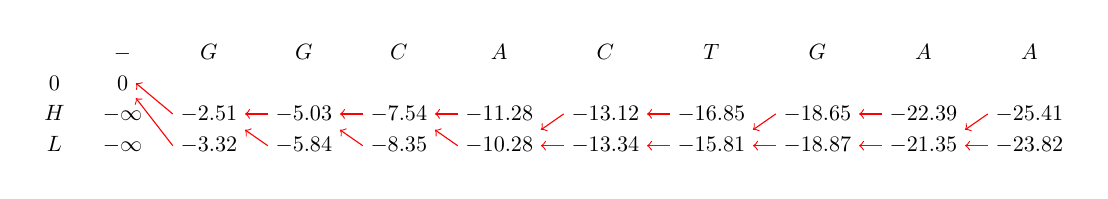
\begin{tikzpicture}[every node/.style={scale=0.8}]
\matrix (m) [matrix of math nodes,column  sep=3mm]
{
 & - & G & G & C & A & C & T & G & A & A \\
 0 &0&&&&&&& \\
H &-\infty &  -2.51 & -5.03 & -7.54 &  -11.28 & -13.12 & -16.85 & -18.65 & -22.39 & -25.41 \\
L &-\infty &-3.32 & -5.84 &  -8.35 & -10.28 & -13.34 & -15.81 & -18.87 & -21.35 & -23.82 \\
};
\draw[draw = red, ->] (m-3-3.west) -- (m-2-2.east);
\draw[draw = red, ->] (m-4-3.west) -- (m-2-2.south east);
\draw[draw = red, ->] (m-3-4.west) -- (m-3-3.east);
\draw[draw = red, ->] (m-3-5.west) -- (m-3-4.east);

\draw[draw = red, ->] (m-3-6.west) -- (m-3-5.east);
\draw[draw = red, ->] (m-3-7.west) -- (m-4-6.north east);
\draw[draw = red, ->] (m-3-8.west) -- (m-3-7.east);
\draw[draw = red, ->] (m-3-9.west) -- (m-4-8.north east);
\draw[draw = red, ->] (m-3-10.west) -- (m-3-9.east);
\draw[draw = red, ->] (m-3-11.west) -- (m-4-10.north east);
\draw[draw = red, ->] (m-4-4.west) -- (m-3-3.south east);
\draw[draw = red, ->] (m-4-5.west) -- (m-3-4.south east);
\draw[draw = red, ->] (m-4-6.west) -- (m-3-5.south east);
\foreach \x/\y in {7/6,8/7,9/8,10/9,11/10}{
\draw[draw = red, ->] (m-4-\x.west) -- (m-4-\y.east);};
\end{tikzpicture}




The first column in this matrix is simple: every sequence is in state 0 at step 0, so $V_0(0) = \log(1) = 0$ while other states have $V_H(0) = V_L(0) = \log(0) = -\infty$.  

The second column is derived from the first as follows: \\ $V_H(1) = \log(e_H(G)) + \max\left\{V_0(0)+\log(a_{0H}),V_H(0)+\log(a_{HH}),V_L(0)+\log(a_{LH})\right\} =  -1.515 + (V_0(0)+log(a_{0H})) = -1.515 - 1 = -2.515$ and similarly for  $V_L(1)$.

Traceback begins in the final column where we see the state that maximises the joint probability is $L$.  Following the pointers from this position and recording the state at each step gives us the state path with the highest probability is $\pi^\ast =  HHHLLLLLL$. Note that  $\pi^\ast$ is built from right to left in the traceback procedure. \sqend



The schematic below shows how the $(i+1)$th column is derived from the $i$th column in a Viterbi matrix.  Here, there are 3 possible states, 1, 2 and 3.  The 0 state is omitted in this diagram. 

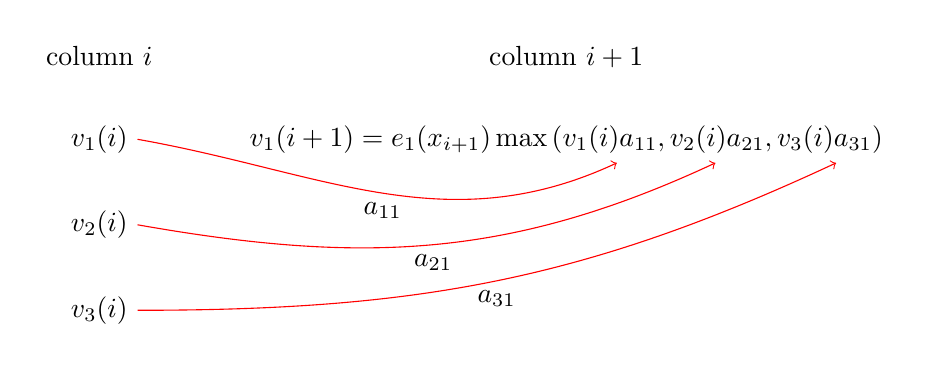
\begin{tikzpicture}
\matrix (m) [matrix of nodes,column sep=10mm,row sep = 5 mm]
{
column $i$ & column $i+1$ \\
  $v_1(i)$ & $ v_1(i+1) = e_1(x_{i+1}) \max\left(v_1(i)a_{11},v_2(i)a_{21},v_3(i)a_{31}\right)$   \\
  $v_2(i)$ &   \\
  $v_3(i)$ &   \\
};
\draw[draw = red, ->] (m-2-1.east) to[out=350,in=205] node[below] {$a_{11}$}(node cs:name = m-2-2,angle = 335)  ;
\draw[draw = red, ->] (m-3-1.east)  to[out=350,in=205] node[below] {$a_{21}$} (node cs:name = m-2-2,angle = 351)  ;
\draw[draw = red, ->] (m-4-1.east) to[out=0,in=205] node[below] {$a_{31}$} (node cs:name = m-2-2,angle = 355)  ;
\end{tikzpicture}

The same diagram shown using log units:

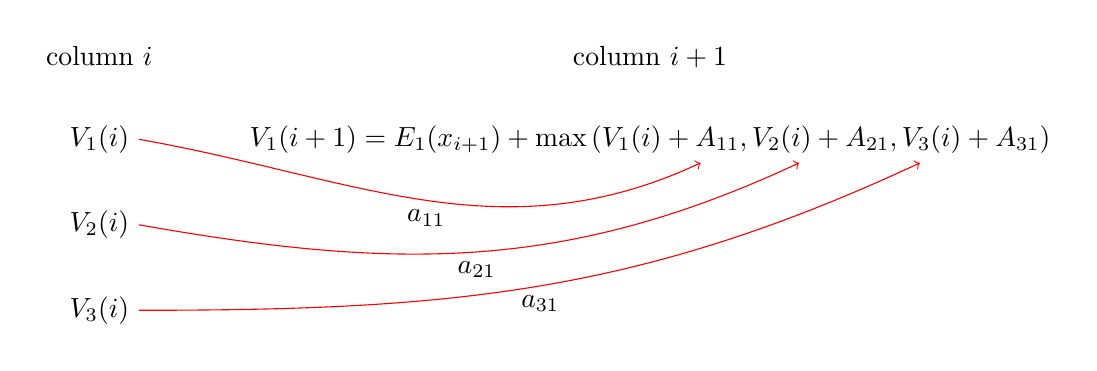
\begin{tikzpicture}
\matrix (m) [matrix of nodes,column sep=10mm,row sep = 5 mm]
{
column $i$ & column $i+1$ \\
  $V_1(i)$ & $ V_1(i+1) = E_1(x_{i+1}) +  \max\left(V_1(i)+A_{11},V_2(i) + A_{21},V_3(i)+ A_{31}\right)$   \\
  $V_2(i)$ &   \\
  $V_3(i)$ &   \\
};
\draw[draw = red, ->] (m-2-1.east) to[out=350,in=205] node[below] {$a_{11}$}(node cs:name = m-2-2,angle = 335)  ;
\draw[draw = red, ->] (m-3-1.east)  to[out=350,in=205] node[below] {$a_{21}$} (node cs:name = m-2-2,angle = 351)  ;
\draw[draw = red, ->] (m-4-1.east) to[out=0,in=205] node[below] {$a_{31}$} (node cs:name = m-2-2,angle = 355)  ;
\end{tikzpicture}


\subsection{The forward algorithm and calculating P(x)}

We have seen that it is easy to calculate $P(x,\pi)$. However, we  usually  only observe $x$ so can't directly calculate  $P(x,\pi)$.   We could tackle this by finding a suitable state path, such as the Viterbi path, $\pi^\ast$, and calculate $P(x,\pi^\ast)$.  But calculating $P(x,\pi^\ast)$ does not adequately tell us the likelihood of observing $x$ which may have arisen from a large number of possible state paths.  

What we really want is calculate is $P(x)$, the probability of observing $x$ without taking any particular state path into account.    This involves marginalizing over all possible paths: that is, 
\[ P(x) = \sum_{\pi} P(x,\pi).\] 
The number of possible state paths grows exponentially so we cannot enumerate them all and naively calculate this sum.  Instead, we use another dynamic programming algorithm called the forward algorithm and calculate $P(x)$ iteratively.  

The forward algorithm iteratively calculates the quantity \[f_k(i) = P(x_{1:i},\pi_i = k),\] the joint  probability  of the  first $i$ observations and the prob that $\pi_i = k$.  The recursion used is that 
\begin{equation} f_l(i+1) = e_l(x_{i+1}) \sum_k f_k(i)a_{kl}. \label{eqn:fwd} \end{equation}
\begin{description}
\item[Initialisation $i = 0$:] $f_0(0) = 1$, $f_k(0) = 0$ for $k>0$.
\item[Recursion $i = 1,\ldots,L$:] $f_l(i) = e_l(x_i) \sum_k  f_k(i-1)a_{kl})$.
\item[Termination:] $P(x) = \sum_k f_k(L)a_{k0}$.
\end{description}
If the end state $0$ is not modelled, simply set $a_{k0} = 1$ to get $P(x) = \sum_k f_k(L)$.

Here's a diagram showing how to get the $(i+1)$th column from the $i$th column in the forward algorithm.  The example shown has three states 1, 2 and 3.

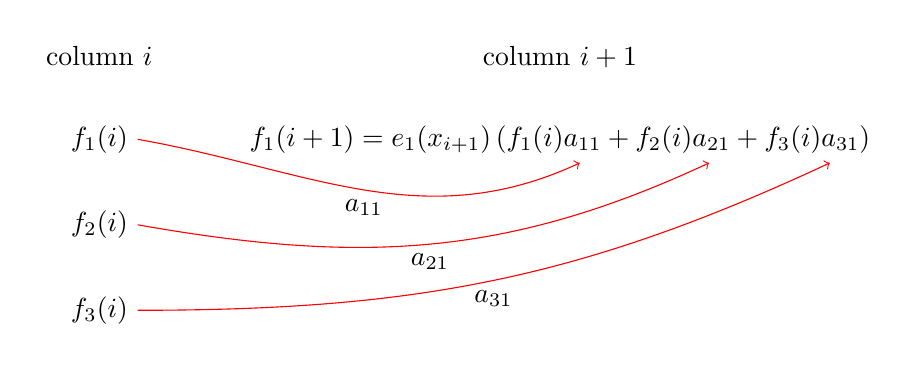
\begin{tikzpicture}
\matrix (m) [matrix of nodes,column sep=10mm,row sep = 5 mm]
{
column $i$ & column $i+1$ \\
  $f_1(i)$ & $ f_1(i+1) = e_1(x_{i+1})\left(f_1(i)a_{11}+f_2(i)a_{21}+f_3(i)a_{31}\right)$   \\
  $f_2(i)$ &   \\
  $f_3(i)$ &   \\
};
\draw[draw = red, ->] (m-2-1.east) to[out=350,in=205] node[below] {$a_{11}$}(node cs:name = m-2-2,angle = 310)  ;
\draw[draw = red, ->] (m-3-1.east)  to[out=350,in=205] node[below] {$a_{21}$} (node cs:name = m-2-2,angle = 351)  ;
\draw[draw = red, ->] (m-4-1.east) to[out=0,in=205] node[below] {$a_{31}$} (node cs:name = m-2-2,angle = 355)  ;
\end{tikzpicture}


Once again, we'll need to work with the log quantities  as the qualities of interest  get very small very fast.  However, if we take the log of both sides of Equation \ref{eqn:fwd}, the log of the sum on the right hand side does not simplify immediately.

Let $F_k(i) = \log(f_k(i))$ and  $A_{kl} = \log(a_{kl})$.  Then Equation  \ref{eqn:fwd} becomes 
\[ F_l(i) = \log [ e_l(x_i) \sum_k  f_k(i-1)a_{kl})]  = \log [ e_l(x_i)] +  \log \left[\sum_k  \exp(F_k(i-1) + A_{kl})\right] \]

Directly calculating a sum of the form $\log(c) = \log(e^a + e^b) $ requires calculating $e^a$ and $e^b$ which we were trying to avoid all along.  Instead, note that $\log(e^a + e^b) = \log(e^a(1 + e^{b-a}) ) = \log(e^a) + \log(1 + e^{b-a}) = a + \log(1 + e^{b-a})$.  If the difference $b-a$ is not too large, this method never need store an extremely large or small number so is numerically stable.  This extends to finding the log of a sum of multiple logged numbers:
\begin{verbatim}
function logsum(x)
  return x[0] + log(sum(exp(x - x[0])))
\end{verbatim}
or, if you are using $\log_2$,
\begin{verbatim}
function log2sum(x)
  return x[0] + log2(sum(2^(x - x[0])))
\end{verbatim}

{\bf Example cont:} For the CG island example above,  use the forward algorithm to calculate the probability of the   sequence $x = GGCACTGAA$.

{\bf Solution:} The matrix produced by the forward algorithm is given below, in log units (base 2).  The first column is based on the start state, 0.  The first entry of the second  column is $log(f_H(1)) = log(e_H(G))  + log(1/2)$

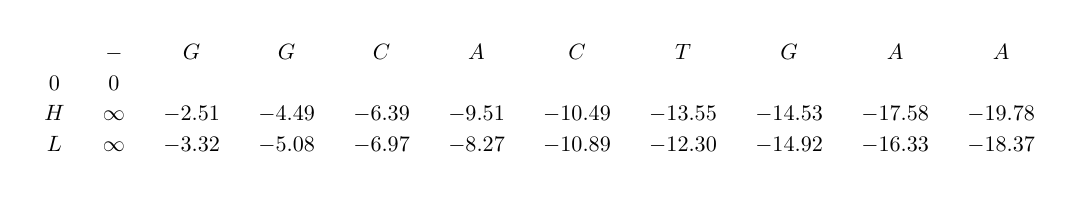
\begin{tikzpicture}[every node/.style={scale=0.8}]
\matrix (m) [matrix of math nodes,column  sep=3mm]
{
 & - & G & G & C & A & C & T & G & A & A \\
 0 &0&&&&&&& \\
H& \infty & -2.51 & -4.49 &-6.39 &-9.51 &-10.49 &-13.55 &-14.53 & -17.58 & -19.78\\
L & \infty &  -3.32 &-5.08 & -6.97 & -8.27 & -10.89 & -12.30 & -14.92 & -16.33 & -18.37\\
};
\end{tikzpicture}

The log probability is thus $\log(P(x)) = \log(2^{-19.78} + 2^{-18.37}) = -17.91$.
 

 
\subsection{The backward algorithm and calculating P(x)}

The backward algorithm is similar and if we run it to the end, we again  calculate $P(x)$.  This starts from the end of the sequence and works back to the beginning.  Define  
\[ b_k(i) = P(x_{(i+1):L} | \pi_i = k)\] 
the probability observing the last part of a sequence, $x_{i+1}, x_{i+2},\ldots,x_L$ conditional on starting in state $k$ at time $i$. 

 

Once again, this is calculated using tabular computation: 
\begin{description}
\item[Initialisation $i = L$:] $b_k(L) = a_{k0}$ for all $k$.
\item[Recursion $i = L-1,\ldots,1$:] $b_k(i) =  \sum_l a_{kl} e_l(x_{i+1}) b_l(i+1)$.
\item[Termination:] $P(x) = \sum_l a_{0l} e_l(x_1) b_l(1)$.
\end{description}
If we don't model the end of the sequence, $a_{k0} = 1$.

Here's a diagram showing how to get the $i$th column from the $(i+1)$th column in the backward algorithm.  The example shown has three states 1, 2 and 3.

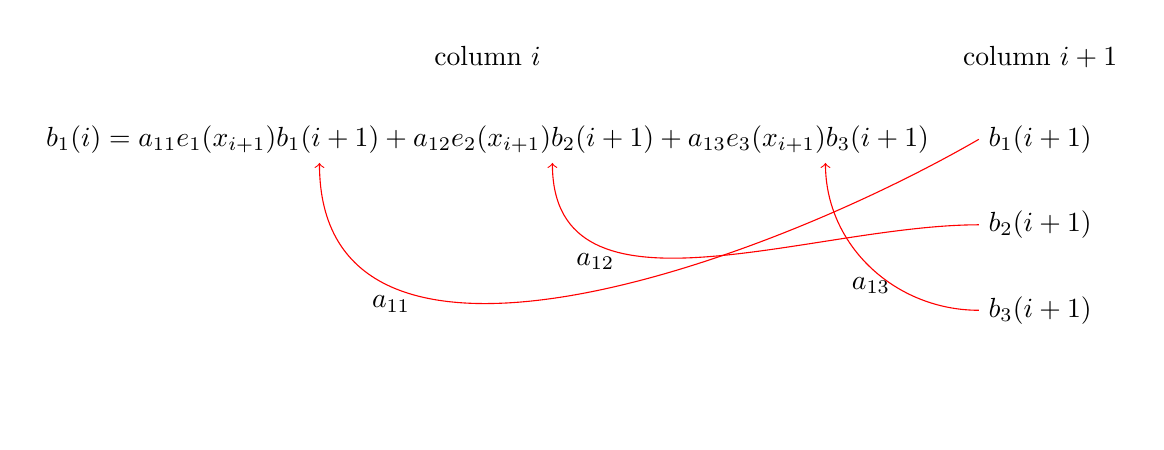
\begin{tikzpicture}
\matrix (m) [matrix of nodes,column sep=2mm,row sep = 5 mm]
{
column $i$ & column $i+1$ \\
  $b_1(i) = a_{11}e_1(x_{i+1})b_1(i+1) + a_{12}e_2(x_{i+1})b_2(i+1) + a_{13}e_3(x_{i+1})b_3(i+1)$  & $b_1(i+1)$   \\
 & $b_2(i+1)$    \\
 & $b_3(i+1)$    \\
};
\draw[draw = red, ->] (m-2-2.west) to[out = 210,in=270] node[pos = 0.75,below] {$a_{11}$}(node cs:name = m-2-1,angle = 188)  ;
\draw[draw = red, ->] (m-3-2.west)  to[out = 180,in=270] node[pos = 0.75,below] {$a_{12}$} (node cs:name = m-2-1,angle = 340)  ;
\draw[draw = red, ->] (m-4-2.west) to[out = 180,in=270] node[below] {$a_{13}$} (node cs:name = m-2-1,angle = 356)  ;
\end{tikzpicture}

The log version of the algorithm is (writing $B_k(i) = \log b_k(i)$):

\begin{description}
\item[Initialisation $i = L$:] $B_k(L) = A_{k0}$ for all $k$ (or $B_k(L) = 0$ if end not modelled)
\item[Recursion $i = L-1,\ldots,1$:] $B_k(i) =  \log \left[ \sum_l \exp(A_{kl} + E_l(x_{i+1}) + B_l(i+1)) \right]$.
\item[Termination:] $P(x) = \log \left[ \sum_l \exp(A_{0l} +  E_l(x_1) + B_l(1)) \right]$.
\end{description}


\subsection{The posterior probability of being in state k at time i $P(\pi_i = k|x)$} \label{sec:probstate}


The final product of this backward algorithm is not usually what we are interested in (we use the forward algorithm to calculate that) but the combined forward and backward algorithms allow us to calculate  the joint  probability  of the all observations and the prob that $\pi_i = k$ 
\begin{eqnarray*}
P(x,\pi_i = k) & =  & P(x_{1:i},\pi_i = k)P(x_{i+1:L}|x_{1:i},\pi_i = k) \mbox{ since } P(A,B) = P(A)P(B|A)\\
 & = &  P(x_{1:i},\pi_i = k)P(x_{i+1:L}|\pi_i = k) \mbox{ by Markov property} \\
 & = &  f_k(i)b_k(i)
\end{eqnarray*}
Of more interest is the posterior probability $P(\pi_i = k | x)$ which we obtain directly by 
\[P(\pi_i = k | x) = \frac{ f_k(i)b_k(i)}{P(x)}, \]
where the denominator is calculated either from the forward or backward algorithm.





\subsection{What can we do with the posterior estimates?}

We saw that the Viterbi path, $\pi^*$, is the most likely single path.  But usually the most likely path is not very likely at all --- there may be many other paths the are nearly as likely.  We can use the posterior $P(\pi_i = k | x)$ to get some other likely paths.

The first is $\hat \pi$, the maximum posterior path, where \[\hat \pi_i =  \argmax_k P(\pi_i = k|x). \]
Note that $\hat \pi$ is often not a legal path through the state space as it may include transitions that are not allowed.

The second is when we are interested in some function of the states, $g(k)$.  In these cases, we calculate the the posterior expectation of $g$ at a particular position, \[G(i|x) = E_k[g(\pi_i |x)] = \sum_k P(\pi_i = k|x)g(k).\]  In particular, if $g$ is an indicator function, that is, $g$ takes the value 1 for some subset of states and 0 for all others, $E_k[g(\pi_i |x)] $ is just the posterior probability that $\pi_i$ is in the specified subset.


\subsection{Estimating the parameters of an HMM}

So far we have assumed we know the structure of the HMM and the associated parameter values (the transition probabilities $a_{kl}$ and emission probabilities $e_k(b)$).  In general, we don't know either of these.  What we usually do is decide on a model (based on our knowledge of the system) and then estimate the parameters of the model.  Let $\theta = \{ a_{kl}, e_k(b)\}$ be the set of all parameters of the model.

Then we are interested in finding the set of parameters that maximizes the (log) likelihood
\[ l(x^1,\ldots,x^n| \theta) = \log P(x^1,\ldots,x^n |\theta) = \sum_{j=1}^n \log P(x^j |\theta). \]
The likelihood of the $j$th sequence,  $ P(x^j |\theta)$, is just what we have been referring to as $P(x^j)$ up to this point as we had always assumed the parameter values, $\theta$, were known.   Writing it as $ P(x^j |\theta)$ simply emphasises the fact that we think of it now as a function of the unknown $\theta$.

If we knew the state paths for a long sequence (or many short sequences), we could estimate the parameters simply by using the empirical proportions of transitions and emissions as our probabilities:
\[\hat a_{kl} = \frac{A_{kl}}{\sum_i A_{ki}} \mbox{ and } \hat e_k(b)\frac{E_k(b)}{\sum_j E_k(j)} \]
where $A$ and $E$ are empirical counts.  Note that, as some transitions or emissions probably wouldn't occur in smaller datasets, it is advisable add a small number of `pseudo-counts' to the empirical counts so that none are zero).  But assuming we know the state paths is unrealistic, so we proceed assuming we have only observed sequences $x^1,x^2,\ldots, x^n $.



\subsection{Baum-Welch algorithm for estimating parameters of HMM}

The Baum-Welch algorithm is an iterative algorithm that attempts to  maximize the (log) likelihood of an HMM.  Unlike earlier algorithms we have seen, it is not exact, so the estimate it finds is not guaranteed to be the best.  It may also get stuck in local maxima, so different starting points are necessary.

The idea of the algorithm is to pick a starting value for $\theta = (a,e)$.  Probable paths for this value of $\theta$ are found.  From these probable paths, a new value for $\theta$ is found by calculating $A$ and $E$. This process repeats until the likelihood of $\theta$ converges on some value (that is, no change or a very small change is seen in $l(x^1,\ldots,x^n| \theta)$ from one step to the next).  
 
In one version of the  algorithm, the probable paths used are the Viterbi paths for each sequence and the values $A$ and $E$ are calculated from these paths. This seems reasonable and can produce satisfactory results but it does not converge to the maximum likelihood estimate.

It turns out that we can avoid actually imputing a probable path by directly calculating the probability that the transition from $k$ to $l$ occurs at position $i$ in $x$: 
\[P(\pi_i = k,\pi_{i+1} = l | x,\theta) = \frac{f_k(i)a_{kl}e_l(x_{i+1})b_l(i+1)}{P(x)}. \]
Thus, to get a the expected value of $A_{kl}$, we simply sum over all possible values of $i$.  A similar argument can be made for $E$.  The expected values for  $A_{kl}$ and $E_{kl}$ are then:
\begin{eqnarray}\label{eqn:AE1}
A_{kl} & = & \sum_j \frac{1}{P(x^j)} \sum_i f_k^j(i) a_{kl} e_l (x_{i+1}^j)b_l^j(i+1) \\
\label{eqn:AE2}
E_k(b) & = & \sum_j \frac{1}{P(x^j)} \sum_{i:x_i^j = b} f_k^j(i)b_k^j(i)
\end{eqnarray}

The Baum-Welch algorithm proceeds as follows:

\begin{description}
\item[Initialise:] Set starting values for the parameters.  Set log-likelihood to $-\infty$.
\item[Iterate:] 
%\renewcommand{\theenumi}{\roman{enumi}}
\begin{enumerate}
\item Set $A$ and $E$ to their pseudo count values.  For each training sequence $x^j$:
\begin{enumerate}
\item Calculate $f_k(i)$ for $x^j$ from forward algorithm
\item Calculate $b_k(i)$ for  $x^j$ from backward algorithm
\item Calculate $A^j$ and $E^j$ and add to $A$ and $E$ using Equations \ref{eqn:AE1} and \ref{eqn:AE2} above.
\end{enumerate}
\item Set new values for $a$ and $e$, based on $A$ and $E$
\item Calculate log-likelihood of model
\item If change in log likelihood is small, stop, else, continue.
\end{enumerate}
\end{description}

See lecture slides for a detailed example of applying the Baum-Welch algorithm.

\subsubsection{Comments on the Baum-Welch algorithm}

The Baum-Welch algorithm is guaranteed to converge to the local maximum ---  exactly which local maximum it converges to depends on the initial state.  Any local maximum is not necessarily the global maximum so the algorithm should be run from multiple different start states to check that a global maximum has been found.  

Also remember that convergence is only guaranteed in the limit of an infinite number of iterations so the exact local maximum is never achieved.  

The algorithm is a type of Expectation-Maximisation (EM) algorithm that is widely used for maximum likelihood estimation.



\subsection{Sampling state paths} \label{sec:sampling}

The probabilities $f_{k}(i)$ we calculate in the forward algorithm can be used to   sample possible state paths in proportion to their probability.  Recall that the Viterbi algorithm provides a method of finding the most probable state path by tracing back though the a matrix, taking the direction that led us to the highest score at each point.  
We adopt the traceback idea but apply it to the matrix $f_k(i)$ and at each step of the traceback, we choose the state in proportion to the amount it contributed to the current probability.  

Assuming an end state is not modelled, the probability of a sequence $x$ is $P(x)  = \sum_k f_k(L)$.  So the probability that the last state is $k$ is given by 
\[P(\pi_L = k |x ) = \frac{f_k(L)}{ \sum_i f_i(L)}. \]
Now, suppose we are in state $l$ at position $i+1$.  We know from the forward algorithm that 
\[ f_l(i+1) = e_l(x_{i+1}) \sum_k f_k(i)a_{kl}. \]
Thus we move to state $k$ in the $i$th position with probability 
\[\frac{f_k(i)a_{kl}} {\sum_j f_j(i)a_{jl} } =  \frac{ e_l(x_{i+1}) f_k(i)a_{kl}} {f_l(i+1)}. \] 
Depending on what you have stored in your algorithm, it may be easier to work with either the left or right hand side of this equation.   

{\bf Example:} Looking again at the CpG island example, sample state paths according to their posterior probabilities for the given sequence $x = TACA$.

{\bf Solution:} First, get the forward matrix, $f$.  To make it simple, don't use the log transform:


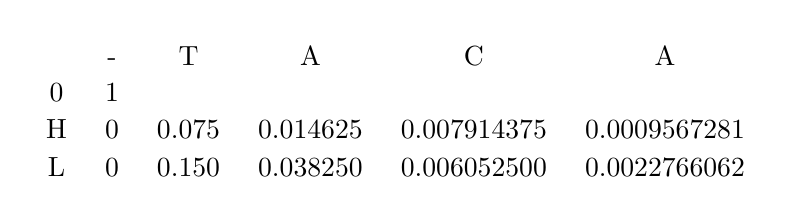
\begin{tikzpicture}
\matrix (m) [matrix of nodes, column sep = 2.5mm]
{
 & - &T&A&C&A \\
 0 & 1 & & & &\\
H & 0 & 0.075 & 0.014625 & 0.007914375& 0.0009567281 \\
L & 0 &0.150 &0.038250 &0.006052500 &0.0022766062 \\
};
\end{tikzpicture}

Now, $P(x) =  \sum_k f_k(L)a_{k0} =   0.003233334$ where $a_{k0} = 1$. So simulate the 4th element of the state path by drawing from $\{H,L\}$ with probabilities $\{ \frac{f_H(4)}{P(x)} = 0.2958952,  \frac{f_L(4)}{P(x)} = 0.7041048 \}$, respectively.  Suppose we sampled $H$.  Then the 3rd element of the state path is a draw from $\{H,L\}$ with respective probabilities 
\[
\left\{ \frac{f_H(3)a_{HH}}{f_H(3)a_{HH} + f_L(3)a_{LH}} =  0.6204251, \frac{f_L(3)a_{LH}}{f_H(3)a_{HH} + f_L(3)a_{LH}}  = 0.3795749\right\}
\]
Suppose we sampled H again.  We now repeat the process, sampling from 
\[
\left\{ \frac{f_H(2)a_{HH}}{f_H(2)a_{HH} + f_L(2)a_{LH}}, \frac{f_L(2)a_{LH}}{f_H(2)a_{HH} + f_L(2)a_{LH}} \right\}
\]
and so on.  We'll end up with a state path, for example, $LLHH$. \sqend

\subsection{HMM model structure}

Defining the correct structure, or `topology', of an HMM is crucial to good estimation but there are no solid rules for doing so.  Usually data is limited so we can't over-parametrise otherwise our estimation algorithms with never find decent values.   So we can't simply allow all possible transitions and let the computer estimate the correct model.  We must decide ourselves, as much as possible, which transition we allow (so that $a_{kl} > 0$) and which we disallow (by setting $a_{kl}=0$).

\subsubsection{Duration modeling}

If we want to accurately model the length of a sequence along with the contents, we  must model an end state as well as the start state.  The basic end state, which is connected to every other state, and has transition probability $q = 1-p$ produces a sequence of length $l$ with probability
\[ P(L = l) = qp^{l-1}. \]
This is a geometric distribution and is the discrete analogue of the exponential distribution.  In general, it is not a very good model for lengths and is used largely for the convenience of its mathematical form.

Also note that the length of time an HMM spends in any one state where the probability of leaving that state is $q$ is geometric.


An easy way to get a more flexible and, perhaps, more realistic distribution of lengths is to have, say, $n$ copies of the HMM linked together  an it stays in each one for a geometrically distributed number of steps.  

An example with 4 states linked together (the states here could be HMMs themselves).
\tikzstyle{block} = [draw,fill=none,minimum size = .7 cm]
\tikzstyle{mydiamond} = [draw,diamond,fill=none]

\begin{tikzpicture}[->, semithick,every text node part/.style={align=center}]
  \tikzstyle{every state}=[fill=none,draw=black,text=black]

        \node[block] at (1,0) (M1) {};
       \node[block] at (3,0) (M2) {};
       \node[block] at (5,0) (M3) {};
       \node[block] at (7,0) (M4) {};
       \node[block,draw = none] at (9,0) (M5) {};
        \draw[->] (M1) [loop above]  to  node [above] {p}  (M1);
        \draw[->] (M2) [loop above]  to node [above] {p} (M2);
        \draw[->] (M3) [loop above]  to node [above] {p} (M3);
        \draw[->] (M4) [loop above]  to node [above] {p} (M4);
        \draw[->] (M1) --  node [below] {q}(M2);
        \draw[->] (M2) --  node [below] {q}(M3);
        \draw[->] (M3) --  node [below] {q}(M4);
        \draw[->] (M4) -- node [below] {q}(M5) ;
        
 \end{tikzpicture}




This produces a negative binomial length distribution, so that 
\[ P(L = l) = {l-1 \choose n-1} p^{l-n}q^n. \]



%%\notinexam{
\section{Applications of HMMs in bioinformatics}
\label{sec:HMMapplication}
\subsection{Pairwise alignment with HMMs}

We saw that we could tackle the pairwise alignment problem with finite  state automata.  We now tackle  the problem using an HMM, which is sometimes called a stochastic FSA.   

We define a {\em pair HMM} as emitting a pair of sequences $(x,y)$ as opposed to the standard HMMs we have considered so far that emit a single sequence.  



The basic HMM which produces a global alignment has three states, $X, Y$ and $M$.  $M$ emits a match, $X$ emits a residue from sequence $x$ and a gap in sequence $y$ (an insertion in $x$ relative to $y$), while $Y$ emits a residue from $y$ and a gap in $x$.   Emission probabilities for states $M,X, Y$ are $p_{x_iy_j}$, $q_{x_i}$ and $q_{y_j}$, respectively.   We also include begin and end states, $B$ and $E$.  Non-zero transition probabilities are $a_{MX} = a_{MY} = \delta$, $a_{XX} = a_{YY} = \epsilon$, $a_{BX} = a_{BY} = \delta$, $a_{kE} = \tau$ for any $k$,  and $a_{kM} \neq 0$ for $k \neq E$ and can be calculated using the fact that $\sum_{k} a_{ik} = 1$.
\begin{figure}
\centering
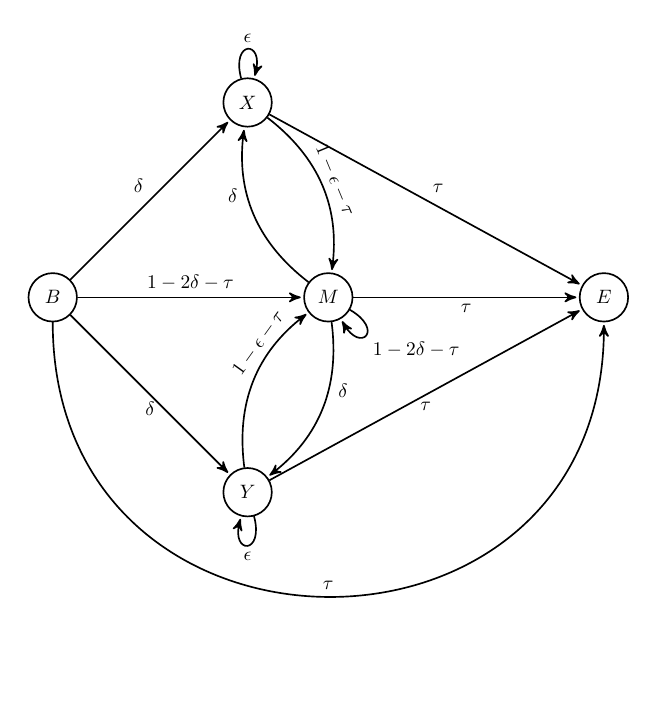
\begin{tikzpicture}[->,>=stealth',shorten >=1pt,auto,node distance=5cm,
                    semithick,every text node part/.style={align=center},scale=0.7, every node/.append style={transform shape}]
  \tikzstyle{every state}=[fill=none,draw=black,text=black]

  \node[state] (B)                    {$ B$};
  \node[state]         (X) [above right of=B] {$X$};
  \node[state]         (M) [ right of=B] {$M$};
  \node[state]         (E) [ right of=M] {$E$};
  \node[state]         (Y) [below right of=B]       {$Y$};

  \path (B) edge              node {$\delta$} (X)
            edge              node  [below] {$\delta$} (Y)
            edge              node {$1-2\delta-\tau$} (M)
            edge [out=270,in=270,looseness=1.7] node {$\tau$} (E)
        (X) edge [loop above] node {$\epsilon$} (X)
        edge  node {$\tau$} (E)
        edge  [bend left] node [sloped] {$1-\epsilon-\tau$} (M)
        (Y) edge [loop below] node {$\epsilon$} (Y)
        edge  node [below] {$\tau$} (E)
        edge  [bend left] node [pos = 0.7,sloped] {$1-\epsilon-\tau$} (M)
        (M) edge [out=330,in=300,looseness=8] node {$1-2\delta-\tau$} (M)
        edge  node [below] {$\tau$} (E)
        edge  [bend left] node [pos = 0.7] {$\delta$} (X)
        edge  [bend left] node [pos = 0.3] {$\delta$} (Y);
 \end{tikzpicture}
 \vspace{-1.5cm}
 \caption{A pair HMM model for global alignment. Emission probabilities for states $M, \, X, \, Y$ are $p_{x_iy_j}$, $q_{x_i}$ and $q_{y_j}$, respectively. Compare it to the simpler FSA in Figure \ref{fig:fsa}.}
 \label{fig:pairhmm}
 \end{figure}

All the algorithms we saw for standard HMMs will work for these pair HMMs but we need a little bit of accounting for the 2 sequences --- instead of $v_k(i)$ or $f_k(i)$, we need to work with $v_k(i,j) $ or $f_k(i,j)$ etc where $k$ is one of the 3 states $M$, $X$ or $Y$.  In each case, we keep 3 score matrices instead of 1 to keep track of which state we are in at every  point in the alignment.

Durbin et al show how the parameters in these pair HMMs work within the Viterbi algorithm to produce exact analogues of the  dynamic programming algorithms we saw earlier.  

For example, to the standard quantities we use in the Needleman-Wunsch algorithm from the Viterbi HMM formulation of global alignment, set 
\begin{align*}
s(a,b) &= \log \frac{p_{ab}}{q_aq_b} + \log{1 - 2\delta - \tau}{(1-\eta)^2} \\
d &= -\log \frac{\delta(1-\epsilon - \tau)}{(1-\eta)(1 - 2\delta - \tau)} \\
e &= -\log \frac{\epsilon}{1-\eta}.
\end{align*}
These pair HMMs give us more than just another way of viewing the basic alignment algorithms.  Since they are couched in the language of probability, we can answer questions about alignments with more depth and nuance than we can with the standard deterministic tools.   


\newpage

\subsubsection{Probability that two sequences are related}

For example, given a pair sequences, $x$ and $y$, we can ask what probability that two sequences are related without relying on any particular alignment.  This is given by the  quantity 
\[ P(x,y) = \sum_\pi P(x,y,\pi) \]
where the sum is over all possible alignments, $\pi$.  As in the standard HMM case, we calculate this quantity via the forward algorithm or the backward algorithm.


\subsubsection{Sampling alignments}

Further, instead of relying on a single alignment, we could sample possible alignments in proportion to their probability using the techniques described in Section \ref{sec:sampling}.

That is, we could calculate the forward $f_M(i,j), \, f_X(i,j)$ and $f_Y(i,j)$ from the forward algorithm and then traceback to find a state path which is an alignment.  The traceback from the current state chooses the next state ($M$, $X$, or $Y$) at each step according to it's contribution to the probability of the current state.    This is exactly the technique described in the Section \ref{sec:sampling}.

\subsubsection{Probability that $x_i$ and $y_j$ are aligned}

Consider two residues,  $x_i$ and $y_j$, in our given sequences $x$ and $y$. What is the probability that they are actually aligned to each other?  Write $\langle x_i,y_j \rangle$ to mean $x_i$ and $y_j$ are aligned, so the probability of interest is $\Pr(\langle x_i,y_j \rangle | x,y)$.  We could estimate this probability by sampling many alignments using the technique described above  and counting the proportion of times that $\langle x_i,y_j \rangle$.  

But it turns out that we can calculate this number exactly using the general technique of finding the posterior probability of being in  a state at some time described in Section \ref{sec:probstate}.  $x_i$ is aligned to $y_j$ exactly when the HMM is in state $M$ at $(i,j)$.  Thus
\[ \Pr(\langle x_i,y_j \rangle | x,y) = P(\pi(i,j)  = M|x,y) = \frac{ P(\pi(i,j)  = M,x,y)}{P(x,y)} = \frac{f_M(i,j)b_M(i,j)}{P(x,y)}. \] 
The last equality is exactly the same as the one derived in Section \ref{sec:probstate} and, as usual, the quantity $P(x,y)$ can be calculated using either the forward or backward algorithm.  







 
 
\subsection{Profile HMMs}

%So far, we have considered sequences in isolation or as pairs.  Typically we deal with many sequences at a time and seek to explain their ancestral relationships and find biologically interesting features of the group of sequences.    As in the two sequence case, we'll need to discuss how to align the group of sequences (this is the problem of multiple sequence alignment) but we'll start by assuming that we are given aligned sequences (a {\em multiple sequence alignment} or MSA) and we want to study properties of the aligned group.  

The canonical  problem in genetics is to find a group of sequences that are homologous.  In particular, we are interested in finding homologous genes that share a similar function.  We say such sequences or genes belong to the same family in the sense that they share a common ancestor and have maintained the same (or similar) functionality. They may be the same sequence in different species or in the same species but in different parts of the genome (having arrived there through duplication).     Sequences in the same family will often have features in common, particularly where they share the same function and, therefore, the same basic secondary structure. 

If we can characterise these families accurately, by finding features that almost certainly share in common and identifying regions where more variation is seen,   we will be able to better align sequences known to belong to the family and  more easily identify other members of the family.  We achieve this characterisation by modelling the family using an HMM, known as a {\em profile HMM}.
 

We'll start by assuming that we are given a family of homologous sequences that are already aligned into a multiple sequence alignment (MSA).  See a very small example in Figure \ref{fig:msa}.




\begin{figure}[htb]
\begin{verbatim}
VGA--HAGEY
V----NVDEV
VEA--DVAGH
VKG------D
VYS--TYETS
FNA--NIPKH
IAGADNGAGV
\end{verbatim}
\vspace{-5mm}
\caption{Ten columns from a given multiple alignment of seven globin sequences.}
\label{fig:msa}
\end{figure}
From a given alignment, we wish to characterise a typical sequence in the alignment at each position.    Once we have made this characterisation, we could use it to search for other sequences (or parts of sequences) that fit the profile and so are candidates to be members of this family.

We model the alignment as an HMM, where each position in the alignment is a state with a distinct probability of emitting the various residues.  

We'll start by supposing the alignment that is largely  free of gaps (by ignoring, say, columns in the alignment that are more than 50\% gaps).
%We can think of  a PSSM giving the emission probabilities for an HMM with a state for each position.  
With each position in the alignment, associate a state in the HMM.   Call this state a match state and label the $i$th match state  $M_i$. The (ungapped) alignment is then modelled as a HMM with only the trivial transitions, $M_i$ to $M_{i+1}$ (with additional begin and end states).   Let emission probabilities from the $i$ match state be  $e_{M_i}$.  A model for a MSA of length 3 looks like:
\tikzstyle{block} = [draw,fill=none,minimum size = .7 cm]
\tikzstyle{mydiamond} = [draw,diamond,fill=none]

\begin{tikzpicture}[->, semithick,every text node part/.style={align=center}]
  \tikzstyle{every state}=[fill=none,draw=black,text=black]

        \node[block] at (0,0) (B) {$B$};
        \node[block] at (2,0) (M1) {$M_1$};
        \node[block] at (4,0) (M2) {$M_2$};
        \node[block] at (6,0) (M3) {$M_3$};
         \node[block] at (8,0) (E) {$E$};
        \draw[->] (B) -- (M1.west);
        \draw[->] (M1.east) -- (M2.west);
        \draw[->] (M2.east) -- (M3.west);
        \draw[->] (M3.east) -- (E.west);

 \end{tikzpicture}

Now let's allow gaps in the alignment.  How do we handle them?  To handle an insertions (with respect to the alignment --- parts of a sequence $x$ that are not matched by anything in the model) we introduce a new set of states $I_i$ which matches the residues in $x$ after $i$ to a gap.  These states have emission probabilities  $e_{I_i}(a)$ which we set to the background rate:  $e_{I_i}(a) = q_a$.

There is a transition from $M_i$ to $I_i$, a loop at $I_i$, and a transition from $I_i$ to $M_{i+1}$.  

\tikzstyle{mydiamond} = [draw,diamond,fill=none,minimum size = 1cm]
\begin{tikzpicture}[->, thick,every text node part/.style={align=center}]
  %\tikzstyle{every state}=[fill=none,draw=black,text=black]
  \tikzstyle{ann} = [draw=none,fill=none,right]

        \node[block] at (0,0) (B) {$B$};
        \node[block] at (2,0) (M1) {};
        \node[block] at (4,0) (M2) {$M_j$};
        \node[mydiamond] at (4,2) (I2) {$I_j$};
        \node[block] at (6,0) (M3) {};
         \node[block] at (8,0) (E) {$E$};
        \draw[->] (B) -- (M1.west);
        \draw[->] (M1.east) -- (M2.west);
        \draw[->] (M2.east) -- (M3.west);
        \draw[->] (M3.east) -- (E.west);
        \draw[->] (M2.north) -- (I2.south);
        \draw[->] (I2.south east) -- (M3.north west);
        \draw[->] (I2) [loop left] to (I2);

 \end{tikzpicture}

A gap of length $k$ therefore has log-odds score 
\[ \log a_{M_iI_i} + \log a_{I_i M_{i+1}} + (k-1)\log a_{I_iI_i}, \] 
the same as an affine gap penalty.

A deletion relative to the model corresponds to skipping ahead in the model.  To allow transitions from every match state to every other state ahead of it in the model would introduce too many transitions (how many would we need?) so we introduce instead a silent delete states $D_i$ next to every match state.  Silent states emit no residues.    We allow transitions $a_{M_{i-1}D_i}, a_{D_{i}M_{i+1}}$ and $a_{D_{i}D_{i+1}}$.  

\tikzstyle{mycircle} = [draw,circle,fill=none,minimum size = 0.7cm]
\begin{tikzpicture}[->, thick,every text node part/.style={align=center}]
  %\tikzstyle{every state}=[fill=none,draw=black,text=black]
  \tikzstyle{ann} = [draw=none,fill=none,right]

        \node[block] at (0,0) (B) {$B$};
        \node[block] at (2,0) (M1) {};
        \node[block] at (4,0) (M2) {$M_j$};
        \node[block] at (6,0) (M3) {};
        \node[mycircle] at (2,2) (D1) {};
        \node[mycircle] at (4,2) (D2) {$D_j$};
        \node[mycircle] at (6,2) (D3) {};
         \node[block] at (8,0) (E) {$E$};
        \draw[->] (B) -- (M1.west);
        \draw[->] (M1.east) -- (M2.west);
        \draw[->] (M2.east) -- (M3.west);
        \draw[->] (D1.east) -- (D2.west);
        \draw[->] (D2.east) -- (D3.west);
        \draw[->] (M3.east) -- (E.west);
        \draw[->] (B.north east) -- (D1.south west);
        \draw[->] (M1.north east) -- (D2.south west);
        \draw[->] (M2.north east) -- (D3.south west);
        \draw[->] (D1.south east) -- (M2.north west);
        \draw[->] (D2.south east) -- (M3.north west);
        \draw[->] (D3.south east) -- (E.north west);
 
 \end{tikzpicture}

A full model incorporates  both insert and delete states and is drawn below.  Notice that we have not drawn transitions between  $I$ and  $D$ states though it simplifies computation to allow them (we'd allow $D_{j} \rightarrow I_{j}$ and $I_{j} \rightarrow D_{j+1}$).


\begin{tikzpicture}[->, thick,every text node part/.style={align=center}]
  %\tikzstyle{every state}=[fill=none,draw=black,text=black]
  \tikzstyle{ann} = [draw=none,fill=none,right]

        \node[block] at (0,0) (B) {$B$};
        \node[block] at (2,0) (M1) {};
        \node[block] at (4,0) (M2) {$M_j$};
        \node[block] at (6,0) (M3) {};
        \node[mycircle] at (2,4) (D1) {};
        \node[mycircle] at (4,4) (D2) {$D_j$};
        \node[mycircle] at (6,4) (D3) {};
         \node[block] at (8,0) (E) {$E$};
         
        \draw[->] (B) -- (M1.west);
        \draw[->] (M1.east) -- (M2.west);
        \draw[->] (M2.east) -- (M3.west);
        \draw[->] (M3.east) -- (E.west);
        \draw[->] (B.north east) -- (D1.south west);
        \draw[->] (M1.north east) -- (D2.south west);
        \draw[->] (M2.north east) -- (D3.south west);
        \draw[->] (D1.south east) -- (M2.north west);
        \draw[->] (D2.south east) -- (M3.north west);
        \draw[->] (D3.south east) -- (E.north west);
 
         \node[mydiamond] at (0,2) (I0) {}; 
         \node[mydiamond] at (2,2) (I1) {};
         \node[mydiamond] at (4,2) (I2) {$I_j$};
         \node[mydiamond] at (6,2) (I3) {};
        \draw[->] (B.north) -- (I0.south);
        \draw[->] (M1.north) -- (I1.south);
        \draw[->] (M2.north) -- (I2.south);
        \draw[->] (M3.north) -- (I3.south);
        \draw[->] (I0.south east) -- (M1.north west);
        \draw[->] (I1.south east) -- (M2.north west);
        \draw[->] (I2.south east) -- (M3.north west);
        \draw[->] (I3.south east) -- (E.north west);
        \draw[->] (I0) [loop left, looseness = 5] to (I0);
        \draw[->] (I1) [loop left, looseness = 5] to (I1);
        \draw[->] (I2) [loop left, looseness = 5] to (I2);
        \draw[->] (I3) [loop left, looseness = 5] to (I3);
        \draw[->] (D1.east) -- (D2.west);
        \draw[->] (D2.east) -- (D3.west);

 \end{tikzpicture}


This profile HMM model is equivalent to a pair HMM model for pairwise alignment where the given MSA is summarised into a single sequence $y$ .  So when we seek to fit a candidate sequence $x$ to our profile HMM, it is as though we are aligning $x$ and $y$ with a pair HMM (with appropriately chosen emission probabilities).  

 
\subsubsection{Estimating the parameters of a profile HMM}

We can choose the parameters of the profile HMM using the empirical counts ($A_{kl}$ and  $E_k(b)$) with pseudo-counts added.   Remember that the number of possible  transitions is limited: in our full drawn model we only allow non-zero transitions for  $a_{M_iM_{i+1}}$,  $a_{M_iD_{i+1}}$, $a_{M_iI_i}$, $ a_{I_iI_i}$, $a_{I_iM_{i+1}}$, $a_{D_iD_{i+1}}$ and $a_{D_iM_{i+1}}$.  We have emissions for all possible residues at each site so we add pseudo-counts to ensure $e_{M_i}(a) > 0$ for all $a$.  Then we use the rule we saw earlier to estimate transition and emission probabilities:
\[a_{kl} = \frac{A_{kl}}{\sum_j A_{kj}} \mbox{ and } e_k(b)  = \frac{E_k(b)}{\sum_j E_k(j)}.\]
A simple way of assigning pseudo-counts is to add 1 to all scores (including zero scores). There is a lengthy discussion of which pseudo-count values to choose in the Durbin et al book and many more sensible schemes are proposed -- none are particularly complicated but we don't have time to cover them all here.

We assume emissions from insert states are at the background rate (that is, that rate the residue occurs at at any position).

In the example in Figure \ref{fig:msa}, the first column has all seven sequences in the match state with 5 Vs, and 1 each of F and I.  The 17 other possible residues are not observed, so have frequency 0.  Adding a pseudo-count of 1 to each observed frequency gives us emission probabilities $e_{M_1}(V) = 6/27$,  $e_{M_1}(F) =  e_{M_1}(I) = 2/27$ and the other 17 residues have  
$e_{M_1}(b) = 1/27$.  6 of the 7 transitions to the next column are to the match state again while one is to a delete state.  Again, adding pseudo-countsof one gives $a_{M_1M_2} = 7/10$, $a_{M_1D_2} = 2/10$ and $a_{M_1I_1} = 1/10$.  Transitions from the insert and delete states are just based on the pseudo-counts here.  



\subsubsection{Finding matches}

Once the model has been set and the parameters estimated, we can set about seeing whether  other sequences match the family.  Call $M$ the model and $x$ a sequence we wish to test against the model.   To do so, we align proposed sequences to the family using the now familiar tools of the Viterbi algorithm, giving the Viterbi path $\pi^*$ (and the associated score, $P(x|\pi^*,M)$) or, better, the full probability of a sequence summed over all alignments, $P(x|M)$.   

These  scores can be used to compare the hypotheses that $x$ belongs to family $M$ or $x$ is no more like $M$ than we would expect at random.  Call $R$ the random model and let  $P(x|R) = \prod_{i = 1}^L q_{x_i}$ be the likelihood of $x$ under the random model where $q_a$ is simply the background rate of occurrence of residue $a$.  If the log ratio $\log (P(x|M)/P(x|R)) > 0$, $x$ is more likely associated with the modelled family than not.  To find more certain matches, we may chose a threshold that this ratio must exceed before we call it a member of the family.


%Instead of log-odds scores, sometimes people simply use log likelihood scores $P(x|M)$ while normalising them  to account for length (simply dividing by length is an easy first step, though it may be easier to fit a curve to the log-likelihood function when considered as a function of length and then consider $Z$-scores).     Sequences that have log-likehood scores that are much higher than a background level are likely members of the modelled family.

Note that if we wish to fit new found sequence $x$ to the family, we can simply use the Viterbi alignment to align it to the family and update parameters of the model. 

\subsubsection{Alignment with a known profile HMM}

The simplest case is when we have a known aligned family to which we have already fitted a profile HMM and we wish to add a number of sequences to the profile.  In this case, we use the Viterbi algorithm to find the most probable alignment for the new sequences.  

The Viterbi path will consist of matches, insert and delete states.   At the delete states, we add a gap character, --, to the sequence we are aligning.  At an insert state, the unaligned residue of the sequence we are aligning is emitted, forcing a gap like character in the already aligned profile.  In the profile, we placeholder character, .\,, at these positions.   Note that if there are multiple insertions in different sequences at a position, there are many ways to align them against each other.   Since we believe insertions are not shared between all members of the family, we can set an arbitrary rule for aligning them, such as using simple left-justification. 

\subsubsection{Alignment from unaligned sequences with HMMs}

If we do not have a pre-existing aligned family and/or profile HMM, we need to first specify an HMM and then use the Baum-Welch algorithm to estimate the parameters.  After we have done that, we are in the same position as above and can construct the MSA from the fitted profile HMM.   

A rule of thumb for specifying the HMM in the absence of prior knowledge is to allow $M$ match states where $M$ is the average length of the training sequences.  
In general, it is difficult  to fit an HMM of this size.  A number of heuristics have been developed to avoid local maxima.  

Clustal$\Omega$  implements this method and is quick enough to align thousands of sequences in reasonable time.  Currently, Clustal$\Omega$ can only be used for protein sequences. See Fabian Sievers et al, 2011, Molecular Systems Biology 7, \url{http://www.nature.com/msb/journal/v7/n1/full/msb201175.html} for a full description.


\subsection{Gene finding}

A DNA sequence can roughly be divided into two types of region: genes and non-genes or inter-genic regions.  Genes are regions that code for proteins which actually perform biological functions in an organism so these regions  are of primary interest.  The role played by  intergenic regions is not yet clear and it is often referred to as `junk DNA'.

We are interested, then, to find a method of finding regions of a given sequence that are genes.  To do so, we need to look at how a gene is structured along a sequence.    Recalling that a sequence has a direction with one end being  5' end, the other being the  3' end. Moving forward in the sequence is going from the 5' end towards the 3' end.  


\begin{figure}[h]
\includegraphics[width=10cm]{figures/genestructure}
\caption{ Gene structure and transcription. The DNA of the coding region is composed of exons (coding DNA) interspersed with introns (non-coding DNA) and is flanked by untranslated regions (UTRs). Upstream of the coding regions within the gene are DNA sequences that control (promoter) and regulate (enhancers) gene expression. During transcription, the initial nuclear transcript includes RNA sequence complementary to the entire coding region and the UTRs. In a subsequent step, the introns are spliced out to form mRNA which translocates to the cytoplasm where it is translated into protein.  Source: \url{http://dx.doi.org/10.1093/bja/aep130} by UoA subscription}
\label{fig:exon}
\end{figure}

Our model of a gene has the following elements occurring in the order listed here: an inter-genic region, a promoter region, a 5' un-transcribed region, a series of {\em exons} and {\em introns}, a 3' un-transcribed region, a poly-A region and then back to another inter-genic region.

These regions are described in more detail below.


Inter-genic region: A non-coding region between genes.

Promoter: a region of DNA that facilitates the transcription of a particular gene. Promoters are located near the genes they regulate, on the same strand and typically upstream (towards the 5' region of the sense strand).
For the transcription to take place, the enzyme that synthesizes RNA, known as RNA polymerase, must attach to the DNA near a gene. Promoters contain specific DNA sequences and response elements that provide a secure initial binding site for RNA polymerase and for proteins called transcription factors that recruit RNA polymerase. These transcription factors have specific activator or repressor sequences of corresponding nucleotides that attach to specific promoters and regulate gene expressions.  

As promoters are typically immediately adjacent to the gene in question, positions in the promoter are designated relative to the transcriptional start site, where transcription of RNA begins for a particular gene (i.e., positions upstream are negative numbers counting back from -1, for example -100 is a position 100 base pairs upstream).

In eukaryotes, the process is complex and promoters may occur hundreds of base-pairs upstream.

In prokaryotes, the promoter consists of two short sequences at -10 (that is 10 bases upstream from the UTR and is called the Pribnow box which typically looks like TATAAT) and at -35 (the -35 element, usually TTGACAT).  The promoter regions are not transcribed to RNA.

Untranslated regions (UTR 5' or 3') :  These are  regions immediately flanking the translated region.   They are transcribed into RNA but not translated into proteins.  

Exons and introns: An exon is transcribed into RNA and is further translated into a protein.  An intron is transcribed into a form of RNA and then spliced out of the RNA sequence that finally gets translated in a protein.  In any gene, there could be one or many exons and zero or many introns.  Exons and introns alternate along the sequence.  

\begin{figure}[h]
\includegraphics[width=10cm]{figures/exonintron}
\caption{A figure showing how the transcribed precursor to messenger RNA includes the UTRs, exons and introns.  The introns are spliced out to form  the messenger RNA.  The Exons in the mRNA are translated into proteins. Souce: \url{http://en.wikipedia.org/wiki/File:Pre-mRNA_to_mRNA.svg} }
\label{fig:exon}
\end{figure}


Poly(A) signal: After the 3' UTR on the RNA, a number of  adenines ($A$s) is added  --- this is called the poly(A) tail.  The poly(A) signal, or polyadenylation signal, is thus a stretch of DNA that signals to the RNA transcription mechanism to begin the addition of the poly(A) tail.  


A method first described in Burge and Karlin 1997 (see \url{http://www.ncbi.nlm.nih.gov/pubmed/9149143}) describes a generalized HMM incorporating all these regions. See Figure \ref{fig:genehmm} for a sketch of the structure of the HMM.  The states of  the HMM are N (corresponding to an inter-genic region), P (promotor), F (5' UTR), E (exons), I (introns), T (3' UTR) and A (poly(A) signal).   The multiple states for  introns, $I_0$, $I_1$ and $I_2$ and exons $E_0$, $E_1$ and $E_2$ indicate the relation of the reading frame of the exon to the reading frame of the initial exon ($E_{init}$).  Recall that three bases of DNA code for a single amino acid, with each group of 3 bases call a codon.  If an exon or intron does not have length that is a multiple of 3, then the start of the next exon or intron may be out of phase with it.  A subscript of 0, 1 or 2 represents in phase or lagging 1 or 2 steps out of phase, respectively.


 
The GHMM produces a set of states $q = q_1\ldots q_n$ with an associated set of lengths (durations) $d = d_1\ldots d_n$ and for each state $q_i$, it produces a sequence of length $d_i$ according to a probability model associated with the state $q_i$.  Algorithms to analyse sequences according to this model are implemented in Genscan and GlimmerHMM. 



\begin{figure}[h]
\includegraphics[width=10cm]{figures/genehmm}
\caption{ The structure of the (generalised) HMM used for gene finding from Burge et al 1997.  See text for details.  The full HMM includes a mirror image corresponding  to the reverse strand which  has been deleted here.  }
\label{fig:genehmm}
\end{figure}

%%}%end not in exam

\clearpage

\newpage


\section{Reconstructing trees}

The fastest ways of constructing trees rely on defining a distance between sequences.  We have already one method that does this: UPGMA in Section \ref{sec:UPGMA}.   We looked at UPGMA in the context of multiple sequence alignment where a sensible choice of  distance between sequeces to use was $D(x,y) = -\log S_{eff}(x,y)$.  We'll briefly look at other, more widely used distance measures.  

\subsection{Defining distances between sequences}

There are numerous ways of defining distances between sequences.  The simplest, for an aligned pair of sequences $x$ and $y$ of length $L$ is to count the number of positions where they differ, $D_{xy}$ say, and define the distance to be  $$f_{xy} = D_{xy}/L,$$ which is simply the fraction of sites at which they differ.  This method works well for  related sequences where $f$ is expected to be small, but doesn't grow as much as we would like as sequences become less and less related since even unrelated sequences share many bases in common due to chance.

The Jukes-Cantor distance is based on the simplest model of sequence evolution where mutations between all four bases are equally likely.  The distance  includes a correction for the fact that unrelated sequences will agree simply due to chance.  The distance is defined by \[d_{xy} = -\frac34 \log {(1- \frac{4f_{xy}}3)}.\] Since the background level of dissimilarity (given by $f_{xy}$) for unrelated sequences is $\frac 3 4$, $(1- \frac{4f_{xy}}3)$ tends to zero as sequences become more unrelated so $d_{xy}$ tends to infinity for unrelated sequences.

\subsection{Ultrametric distances}

UPGMA produces the correct tree (i.e., produces the tree along which the sequences actually evolved) if  the sequences evolved according to a {\em molecular clock} in which sequences evolved at a constant rate over the whole tree.      In that case, the number of mutations is  proportional to the temporal distance of a node to the ancestor. 

In these cases, the distances are said to be {\em ultrametric} and UPGMA will reconstruct the correct tree.  The ultrametric condition is that $d_{ij}$ is ultrametric when, for and points $i,j,k$, the distances $d_{ij}, d_{jk},d_{ik}$ are either all equal or two are equal and the remaining one is smaller.  

More simply, in an ultrametric tree, the distance from the root to the leaves is the same for every leaf.  So  if all leaf nodes are sampled at the same time and the ultrametric property holds, the tree displaying the distances will have all the leaf nodes at the same level.

\tikzset{vertex/.style = {circle, draw, fill=black!50,inner sep=0pt, minimum width=4pt}}
\tikzset{point/.style = {inner sep=0pt, minimum width=0pt}}
\begin{tikzpicture}[thick,y=4cm ]
    \node [vertex] at (0,0) (A) {} ;
    \node [vertex] at (2,0) (B) {} ;
    \node [vertex] at (3,0) (C) {} ;
    \node [vertex] at (4,0) (D) {} ;
    \node [point] at (0,0.5) (E) {} ;
    \node [point] at (2,0.5) (F) {} ;
    \node [point] at (1.5,0.6) (G) {} ;
    \node [point] at (3.5,0.6) (H) {} ;
    \node [point] at (3,0.5) (I) {} ;
    \node [point] at (4,0.5) (J) {} ;
    \node [point] at (1.5,0.5) (K) {} ;
    \node [point] at (3.5,0.5) (L) {} ;
             
     \path (A) edge  (E);
     \path (E) edge (F);
     \path (F) edge  (B);
     \path (G) edge (K);
     \path (G)  edge (H);
     \path (H) edge (L);
     \path (I) edge (J);
     \path (I) edge (C);
     \path (J) edge  (D);
\end{tikzpicture}\hspace{2cm}
\begin{tikzpicture}[thick,y=4cm ]
    \node [vertex] at (0,0) (A) {} ;
    \node [vertex] at (2,0.4) (B) {} ;
    \node [vertex] at (3,0.4) (C) {} ;
    \node [vertex] at (4,0) (D) {} ;
    \node [point] at (0,0.5) (E) {} ;
    \node [point] at (2,0.5) (F) {} ;
    \node [point] at (1.5,0.6) (G) {} ;
    \node [point] at (3.5,0.6) (H) {} ;
    \node [point] at (3,0.5) (I) {} ;
    \node [point] at (4,0.5) (J) {} ;
    \node [point] at (1.5,0.5) (K) {} ;
    \node [point] at (3.5,0.5) (L) {} ;
             
     \path (A) edge  (E);
     \path (E) edge (F);
     \path (F) edge  (B);
     \path (G) edge (K);
     \path (G)  edge (H);
     \path (H) edge (L);
     \path (I) edge (J);
     \path (I) edge (C);
     \path (J) edge  (D);
\end{tikzpicture} \\
The tree on the left is ultrametric, the tree on the right is not.



In most cases, the ultrametric assumption is not a good one, as different regions of sequences vary at different rates and different lineages of the tree may have different rates of mutation.  Thus, UPGMA will not reconstruct the correct tree in most cases.

\subsection{Additive distances}

A less stringent condition is that distances are {\em additive}.  A tree is said to have additive edge lengths if the distance between two leaves is the sum of the edge lengths connecting them.  You can show that ultrametric distances are additive but the reverse does not hold.  In an additive tree, the {\em four point condition} is satisfied, in which any four leaves can be relabelled so that $d(x,y) + d(u,v) \leq d(x,u)+ d(y,v) = d(x,v)+ d(y,z)$.

A set of additive distance can be thought of as tree-like --- there is a tree that correctly displays those distance as branch lengths. 

So the question is, given a set of additive distances, can we reconstruct the correct tree?


\subsection{Neighbour joining}

The answer turns out to be yes, and the algorithm that lets us achieve this is known as {\em neighbour joining} (NJ).  NJ is similar to UPGMA but instead of simply using a pairwise evolutionary distance matrix, NJ takes that matrix as a starting point and then builds a rate-corrected distance matrix before proceeding to join nearest neighbours.

First, note that to find the nearest neighbour on a tree, it is not sufficient to simply calculate the smallest distance.   

{\bf Example:} Consider the tree 

\tikzset{vertex/.style = {circle, draw, fill=black!50,inner sep=0pt, minimum width=4pt}}
\tikzset{point/.style = {inner sep=0pt, minimum width=0pt}}
\begin{tikzpicture}[thick,y=6cm ]
    \node [vertex,label = below:$A$] at (0,0) (A) {} ;
    \node [vertex,label = below:$B$] at (2,0.4) (B) {} ;
    \node [vertex,label = below:$C$] at (3,0.4) (C) {} ;
    \node [vertex,label = below:$D$] at (4,0) (D) {} ;
    \node [point] at (0,0.5) (E) {} ;
    \node [point] at (2,0.5) (F) {} ;
    \node [point] at (1.5,0.6) (G) {} ;
    \node [point] at (3.5,0.6) (H) {} ;
    \node [point] at (3,0.5) (I) {} ;
    \node [point] at (4,0.5) (J) {} ;
    \node [point] at (1.5,0.5) (K) {} ;
    \node [point] at (3.5,0.5) (L) {} ;
             
     \path (A) edge  node[left] {$0.5$}  (E);
     \path (E) edge (F);
     \path (F) edge  node[left] {$0.1$}(B);
     \path (G) edge node[left] {$0.1$}(K);
     \path (G)  edge (H);
     \path (H) edge node[left] {$0.1$}(L);
     \path (I) edge (J);
     \path (I) edge  node[left] {$0.1$}(C);
     \path (J) edge  node[left] {$0.5$} (D);
\end{tikzpicture}

from which we derive the pairwise distance matrix  
\[ d = \bordermatrix{~ & A & B & C & D \cr
              A & 0 & 0.6 & 0.8 & 1.2 \cr
              B &  & 0 & 0.4 & 0.8 \cr
              C &  &  & 0 & 0.6 \cr
              D &  &  &  & 0 \cr}.
\]
If we try to reconstruct the tree using UPGMA, the first step is to choose the pair with the smallest distance and join them. That  has us choosing B and C first as sharing a common ancestor before anything else.  This immediately leads to the the wrong tree topology.  \sqend

To find the nearest neighbour instead of just the node at the smallest distance, we need to subtract the average distance to all other leaves.  Let
$D_{ij} = d_{ij} - (r_i + r_j)$ where 
\[ r_i = \frac1{|L| - 2} \sum_{k\in L} d_{ik} \]
and $L$ is the number of leaves (sequences).  Note that the denominator in calculating $r$ is deliberately one less than the number of items summed.  It can be shown (with a bit of work, omitted here) that the pair of leaves $i,j$ for which $D_{ij}$ is minimal are  neighbouring leaves.  

This leads us to the NJ algorithm, which progressive builds up a tree $T$ by keeping a list of active nodes $L$ and finding the closest amongst them.

\subsubsection*{Neighour joining algorithm}

\begin{enumerate}
\item Let $T$ be the set of all leaf nodes and set $L = T$.
\item Iterate  until $|L| = 2$: 
\begin{enumerate} 
\item Calculate (or update) $D$ from the distance matrix  $d$.
\item Pick $i,j$ for which $D_{ij}$ is minimal.
\item Define $k$ so that $d_{km} = \frac12(d_{im} + d_{jm} - d_{ij})$ for all $m \in L$.
\item Add $k$ to $T$ with edges joining to $i$ and $j$ with lengths $d_{ik} =\frac12(d_{ij} + r_i - r_j) $ and $d_{jk}  = d_{ij} - d_{ik}.$
\item Set $L = L - \{i,j\} + {k}$.
\end{enumerate}
\item $|L| = 2$, so add remaining edge connect $i,j$ with length $d_{ij}$.
\end{enumerate}
To see this works, consider the reverse process where we strip away leaves from an additive tree by removing neighbouring pairs.  Find leaves $i,j$ with parent $k$.  Remove $i,j$ and add $k$ to the list of leaves, defining $d_{km} = \frac12(d_{im} + d_{jm} - d_{ij})$ where $m$ is some other leaf node.   

\begin{figure}[hbtp]
\includegraphics[width=11cm]{figures/nj}
\caption{ Example from wikipedia \url{http://en.wikipedia.org/wiki/Neighbor_joining}: Starting with a star tree in which all leaf nodes are active (A).  The matrix $D$ is calculated and used to choose a pair of nodes for joining, in this case f and g. These are joined to a newly created node, u, as shown in (B). The part of the tree shown as dotted lines is now fixed and will not be changed in subsequent joining steps. The distances from node u to the nodes a-e are computed from the formula given in the text. This process is then repeated, using a matrix of just the distances between the nodes, a,b,c,d,e, and u, and a new D matrix derived from it. In this case u and e are joined to the newly created v, as shown in (C). Two more iterations lead first to (D), and then to (E), at which point the algorithm is done, as the tree is fully resolved.}
\label{fig:nj}
\end{figure}


{\bf Example:}  Perform neighbour joining on the distance matrix from the previous example  
\[ d = \bordermatrix{~ & A & B & C & D \cr
              A & 0 & 0.6 & 0.8 & 1.2 \cr
              B &  & 0 & 0.4 & 0.8 \cr
              C &  &  & 0 & 0.6 \cr
              D &  &  &  & 0 \cr}.
\]

{\bf Solution:} We first need to calculate $D$ for which we will need $r$.  Here $L = 4$, so  
\[ r_A = \frac 1 2 (d_{AB} + d_{AD}  + d_{AD}) = \frac 1 2 (0.6 + 0.8  + 1.2) = 2.6/2 = 1.3. \]
Get other elements of $r$ similarly so $r = (1.3, 0.9, 0.9, 1.3)$.  

From $r$ and $d$ we can thus calculate 
\[ D= \bordermatrix{~ & A & B & C & D \cr
A & - &-1.6 &-1.4 &-1.4 \cr
B &-  &- &-1.4 &-1.4 \cr
C &- &- & - &-1.6\cr
D &- &- &-& -\cr}.
\]
$D$ is symmetric and the diagonal is irrelevant so only need calculate either the elements of the upper or lower traingle.  

The minimum value of the rate-adjusted matrix is found at $AB$ and $CD$.  Choose $AB$ to merge into new node $E$.  The length of the edge from $A$ to $E$ is $d_{AE} = \frac12(d_{AB} + r_A - r_B) = \frac12(0.6 + 1.3 - 0.9 ) = 0.5$ while the distance from $B$ to $E$ is found by $d_{AE}  = d_{AB} - d_{AE} = 0.6 - 0.5 = 0.1$.  Check these branch lengths against the values in the original tree: they match.

$A$ and $B$ can now be removed from the leaf set and replaced with $E$ and a new rate adjusted matrix $D$ derived. Completing a further iteration and the final step reconstructs the original tree. \sqend


\subsubsection{Unrooted vs rooted trees}

Notice that the neighbour-joining algorithm produces a tree with no root.  That is, we known branch lengths (in terms of distance between sequences --- roughly, the number of changes along a branch) but we don't know the actual times of the nodes, so we don't know the position of the root.  A tree with no root is an  {\em unrooted tree} and a tree with a known root position is called a {\em rooted tree}.  

In some cases we can determine the position of the root by including a known {\em out-group} in the analysis.  For example, if we have samples from 20 hominids, we could include a chimp as an out-group since we know that the hominids all share a recent common ancestor before the most recent common ancestor of hominids and chimps.    In this example, we would place the root on the branch separating the chimp from the hominids.

The number of trees, rooted or unrooted is huge.  If we have $n$ taxa, there are 
\[ \frac{(2n-5)!}{2^{n-3}(n-3)!}\] 
unrooted trees and
\[ \frac{(2n-3)!}{2^{n-2}(n-2)!}\]
rooted trees. So when $n=5$, we have 15 unrooted and 105 rooted trees, but for $n=10$ there are about 2 million unrooted and 3.5 million rooted trees.


\subsubsection{Complexity of neighbour jointing and UPGMA}

UPGMA has time and space complexity of $O(n^2)$ while neighbour-joining has the same space complexity but time complexity of $O(n^3)$.  

However, these are worst case complexities, and there are various heuristics that result in average time performance for neighbour-joining appears somewhat better than $O(n^3)$.




\subsection{Parsimony}

Parsimony is  form of Occam's razor. It postulates that the best tree is the one that requires the fewest changes along it to explain all sequences.  This best tree is called the most parsimonious tree or the {\em (maximum)  parsimony tree}.  

The main algorithm that we discuss here is not actually a method for constructing the maximum parsimony tree  but rather provides a way of calculating the cost of any given tree.  We must then search over trees to find the tree of minimal cost.

{\bf Example:} suppose we have four sequences $AAG, AAA, GGA$ and $AGA$.  Consider the two trees given below.

\tikzset{vertex/.style = {circle, draw, fill=black!50,inner sep=0pt, minimum width=4pt}}
\tikzset{point/.style = {inner sep=0pt, minimum width=0pt}}
\begin{tikzpicture}[thick,y=6cm,x = 2cm ]
    \node [vertex,label = below:$AAG$] at (0,0) (A) {} ;
    \node [vertex,label = below:$AAA$] at (1,0) (B) {} ;
    \node [vertex,label = below:$GGA$] at (2,0) (C) {} ;
    \node [vertex,label = below:$AGA$] at (3,0) (D) {} ;
    \node [point] at (0,0.3) (E) {} ;
    \node [point] at (1,0.3) (F) {} ;
    \node [point] at (0.5,0.6) (G) {} ;
    \node [point] at (2.5,0.6) (H) {} ;
    \node [point] at (2,0.3) (I) {} ;
    \node [point] at (3,0.3) (J) {} ;
    \node [point,label = below:{AAA}] at (0.5,0.3) (K) {} ;
    \node [point,label = below:{AGA}] at (2.5,0.3) (L) {} ;
             
     \path (A) edge  node[left] {1}  (E);
     \path (E) edge (F);
     \path (F) edge (B);
     \path (G) edge    (K);
     \path (G)  edge node[below] {AAA} (H);
     \path (H) edge node[left] {1} (L);
     \path (I) edge (J);
     \path (I) edge node[left] {1}  (C);
     \path (J) edge (D);

\end{tikzpicture}
\begin{tikzpicture}[thick,y=6cm,x = 2cm ]
    \node [vertex,label = below:$AAG$] at (0,0) (A) {} ;
    \node [vertex,label = below:$AGA$] at (1,0) (B) {} ;
    \node [vertex,label = below:$AAA$] at (2,0) (C) {} ;
    \node [vertex,label = below:$GGA$] at (3,0) (D) {} ;
    \node [point] at (0,0.3) (E) {} ;
    \node [point] at (1,0.3) (F) {} ;
    \node [point] at (0.5,0.6) (G) {} ;
    \node [point] at (2.5,0.6) (H) {} ;
    \node [point] at (2,0.3) (I) {} ;
    \node [point] at (3,0.3) (J) {} ;
    \node [point,label = below:{AAA}] at (0.5,0.3) (K) {} ;
    \node [point,label = below:{AAA}] at (2.5,0.3) (L) {} ;
             
     \path (A) edge node[left] {1}  (E);
     \path (E) edge (F);
     \path (F) edge node[left] {1} (B);
     \path (G) edge (K);
     \path (G)  edge node[below] {AAA} (H);
     \path (H) edge (L);
     \path (I) edge (J);
     \path (I) edge (C);
     \path (J) edgenode[left] {2}  (D);

\end{tikzpicture}\\
The number of mutations on each branch is shown to the left of the branch.  The tree topology on the left has requires 3 mutations to explain the given sequences, while the tree on the right requires 4 mutations to explain the same sequences.  The more parsimonious tree is therefore the one on the left.   The sequences given at the internal vertices and the positions of the mutations could be altered in these examples but the total parsimony score for each tree would remain the same. \sqend



An algorithm to compute the parsimony cost of a tree is given below.  This finds the minimum number of substitutions to explain given sequences and tree.  It assumes that all changes have equal cost. A similar algorithm accounts for the case where different substitutions have different costs.  The algorithm is given in terms of rooted trees but the parsimony score is independent of the position of the root so this algorithm applies to unrooted trees.


\subsubsection*{Parsimony (Fitch 1971)}

Number the nodes, in descending order, so that the root node is $2n-1$.  Let $u$ be the site for which we are considering the cost. Let $B$ be the parsimony cost.

\begin{description}
\item[Initilise] Set $B_u = 0$ and $k = 2n-1$.
\item[Recursion] To obtain the set $R_k$:

If $k$ is a leaf node: Set $R_k = x^k_u$.

If $k$ is not a leaf: compute $R_i$ and $R_j$ for child nodes of $k$.  Set $R_k = R_i \cap R_j$ if $R_i \cap R_j \neq \emptyset$.  Otherwise,  set $R_k = R_i \cup R_j$ and set $B_u = B_u+1$.
\item[Stop] Return  $B_u$, the minimal cost of the tree at site $u$.
\end{description}



A traceback procedure can be used to construct possible ancestral states.  Starting at the root, choose a residue from $R_{2n-1}$ and go to the daughter nodes.  Having chosen a residue at $R_k$, pick the same residue from the child set $R_i$ if possible, otherwise choose a random reside of $R_i$.  

The total cost for a tree and sequences is the sum of costs over all positions in the sequence. That is, if we have sequences of length $L$ and $B_i$ is the parsimony score for site $i$, then the total parsimony score for the tree and sequences is 
\[ B = \sum_{i = 1}^L B_i. \]

{\bf Example:} Given the following tree with just a single site at the 4 leaves we want to calculate the parsimony cost.   Label the nodes as shown.  There is just a single site so set $u = 1$.  

\tikzset{vertex/.style = {circle, draw, fill=black!50,inner sep=0pt, minimum width=4pt}}
\tikzset{point/.style = {inner sep=0pt, minimum width=0pt}}
\begin{tikzpicture}[thick,y=6cm,x = 1.5cm ]
    \node [vertex,label = below: 1: $A$] at (0,0) (A) {} ;
    \node [vertex,label = below: 2: $G$] at (1,0) (B) {} ;
    \node [vertex,label = below: 3: $C$] at (2,0) (C) {} ;
    \node [vertex,label = below: 4: $C$] at (3,0) (D) {} ;
    \node [point] at (0,0.3) (E) {} ;
    \node [point] at (1,0.3) (F) {} ;
    \node [point] at (0.5,0.6) (G) {} ;
    \node [point] at (2.5,0.6) (H) {} ;
    \node [point] at (2,0.3) (I) {} ;
    \node [point] at (3,0.3) (J) {} ;
    \node [point,label = below:{5}] at (0.5,0.3) (K) {} ;
    \node [point,label = below:{6}] at (2.5,0.3) (L) {} ;
    \node [point,label = below:{7}] at (1.5,0.6) (R) {x} ;
             
     \path (A) edge node[left] {}  (E);
     \path (E) edge (F);
     \path (F) edge node[left] {} (B);
     \path (G) edge (K);
     \path (G)  edge node[below] {} (H);
     \path (H) edge (L);
     \path (I) edge (J);
     \path (I) edge (C);
     \path (J) edgenode[left] {}  (D);
\end{tikzpicture}\\

We set $B = 0$ and $k = 7$.  Now try to find $R_7$.  

7 is not a leaf node, so recurse down to its children.  Want to find $R_5$ and $R_6$. 5 is not a leaf node so recurse down to its children.  1 is a leaf node so set $R_1 = \{ A\} $.  Similarly, $R_2 = \{ G \}$. Now, $R_1 \cap R_2  = \emptyset$ so we set $R_5 = R_1 \cup R_2 = \{ A, G \}$ and $B = B+1  = 0+1 = 1$.

In a similar manner we get $R_3 = \{ C \} $ and $R_4 = \{ C \}$ so $R_6 = R_3 \cap R_4 = \{ C \}$. 

Now, since $R_5 \cap R_6 = \emptyset$ we set $R_7 = R_5 \cup R_6 = \{A, C, G \}$ and $B = B+1 = 2$.

Thus we have the sets $R_k$ as follows:

\tikzset{vertex/.style = {circle, draw, fill=black!50,inner sep=0pt, minimum width=4pt}}
\tikzset{point/.style = {inner sep=0pt, minimum width=0pt}}
\begin{tikzpicture}[thick,y=6cm,x = 2cm ]
    \node [vertex,label = below:  $R_1 \equiv  \{A\}$] at (0,0) (A) {} ;
    \node [vertex,label = below:  $R_2 \equiv  \{G\}$] at (1,0) (B) {} ;
    \node [vertex,label = below:  $R_3 \equiv  \{C\}$] at (2,0) (C) {} ;
    \node [vertex,label = below:  $R_4 \equiv  \{C\} $] at (3,0) (D) {} ;
    \node [point] at (0,0.3) (E) {} ;
    \node [point] at (1,0.3) (F) {} ;
    \node [point] at (0.5,0.6) (G) {} ;
    \node [point] at (2.5,0.6) (H) {} ;
    \node [point] at (2,0.3) (I) {} ;
    \node [point] at (3,0.3) (J) {} ;
    \node [point,label = below: {\{A,G\} }] at (0.5,0.3) (K) {} ;
    \node [point,label = below:{\{C \} }] at (2.5,0.3) (L) {} ;
    \node [point,label = below:{\{A,C,G\} }] at (1.5,0.6) (R) {x} ;
             
     \path (A) edge node[left] {}  (E);
     \path (E) edge (F);
     \path (F) edge node[left] {} (B);
     \path (G) edge (K);
     \path (G)  edge node[below] {} (H);
     \path (H) edge (L);
     \path (I) edge (J);
     \path (I) edge (C);
     \path (J) edgenode[left] {}  (D);
\end{tikzpicture}\\
From these sets, we can traceback from the root, picking possible ancestral states that would give us the parsimony score for the tree.  For example, at the root choose $A$, which forces us to choose $A$ at node 5.  Clearly, at node 6, we only have the choice of $C$.

\tikzset{vertex/.style = {circle, draw, fill=black!50,inner sep=0pt, minimum width=4pt}}
\tikzset{point/.style = {inner sep=0pt, minimum width=0pt}}
\begin{tikzpicture}[thick,y=6cm,x = 2cm ]
    \node [vertex,label = below:  $ A$] at (0,0) (A) {} ;
    \node [vertex,label = below:  $G$] at (1,0) (B) {} ;
    \node [vertex,label = below:  $C$] at (2,0) (C) {} ;
    \node [vertex,label = below:  $C $] at (3,0) (D) {} ;
    \node [point] at (0,0.3) (E) {} ;
    \node [point] at (1,0.3) (F) {} ;
    \node [point] at (0.5,0.6) (G) {} ;
    \node [point] at (2.5,0.6) (H) {} ;
    \node [point] at (2,0.3) (I) {} ;
    \node [point] at (3,0.3) (J) {} ;
    \node [point,label = below: $A$] at (0.5,0.3) (K) {} ;
    \node [point,label = below: $C$] at (2.5,0.3) (L) {} ;
    \node [point,label = below: $A$] at (1.5,0.6) (R) {x} ;
             
     \path (A) edge node[left] {}  (E);
     \path (E) edge (F);
     \path (F) edge node[left] {} (B);
     \path (G) edge (K);
     \path (G)  edge node[below] {} (H);
     \path (H) edge (L);
     \path (I) edge (J);
     \path (I) edge (C);
     \path (J) edgenode[left] {}  (D);
\end{tikzpicture} \sqend

%%% \notinexam{
\subsubsection{Weighted parsimony}

The basic parsimony idea easily extends to the case where instead of counting each mutation equally, different costs apply to  different mutations.

Let $S(a,b)$ be the cost of mutating from $a$ to $b$ and again calculate the  parsimony score at a single site $u$.

\begin{description}
\item[Initilise] Set $k = 2n-1$.
\item[Recursion] 

If $k$ is a leaf node:  Set $S_k(a) = 0$ when $a =  x^k_u$ and  $S_k(a) = \infty$ otherwise.

If $k$ is not a leaf: Compute $S_i(a)$ and $S_j(a)$ for all $a$ and children $i$ and $j$ of $k$.  
Set $$S_k(a) = \min_b \left(S_i(b) +S(a,b)\right) + \min_b \left(S_j(b) + S(a,b)\right).$$

\item[Stop] Return  $$B_u = \min_a S_{2n-1}(a).$$
\end{description}


The total cost of the tree is $$B = \sum_{u = 1}^L B_u$$

Weighted parsimony reduces to the standard parsimony algorithm when $S(a,a) = 1$ and $S(a,b) = 0$ if $a \neq b$.

A traceback procedure to recover the ancestral states is again available by keeping track of which residue, $b$, gave the minimum at each step.   For exact details of the traceback, see Durbin et al.

%%}%end not in exam



\subsubsection{Parsimony informative sites}

Many sites in an alignment will have the same parsimony score on every tree.  For example, consider sites that have the same residue for all taxa (an invariant site).  This will have a parsimony score of 0 regardless of the tree.  Sites that have different scores on different trees are known as {\em parsimony informative}.  It is easy to show that parsimony informative sites have at least two characters that each occur in two or more taxa.   

In the detailed example given above, the site studied (which would be written as the column AGCC in a multiple sequence alignment for the 4 taxa) is not parsimony informative since there is only one site that appears more than once.    If we instead considered the site corresponding to the column $AACC$, it would be parsimony informative.
 


\subsection{Finding the maximum parsimony  tree}

The number of substitutions on a tree (the parsimony score) is sometimes called the {\em length}  of a tree.  This corresponds to the molecular clock idea where, under a constant rate mutation model, we will only see more substitutions if we wait for a longer time.  

Thus finding the maximum parsimony tree is equivalent to finding the shortest tree.  We'll consider a number of methods for finding the maximum parsimony tree for a given set of sequences.


\subsubsection{Exhaustive search}

Finding the maximum parsimony tree is a very hard problem computationally.  Naive methods which attempt to score all possible unrooted trees fail when the number of sequences is even moderate due the huge number of possible trees. 



We therefore need to resort to more clever methods and heuristic  search algorithms.  

 The simplest of the smarter search algorithms are based on the idea of branch-and-bound. % These methods that rule out large numbers of possible trees quickly and efficiently by stopping when the parsimony score exceeds some upper bound.   





(The following section of notes on parsimony is based on notes from \url{http://www.fos.auckland.ac.nz/~biosci742/4_3_2.html#4.3.4})

\subsubsection{Branch and bound}


\begin{figure}[hbtp]
\includegraphics[width=14cm]{figures/parsimony}
\caption{ Say we have sequences from 5 taxa. We start by building the single 3-taxon tree using taxa A, B and C (tree a). Next the fourth taxon D is added in all three possible positions to generate trees b1, b2, and b3. One of these trees, say b1, is chosen. Then the fifth taxon E is added in all possible positions to give trees c1.1, c1.2, c1.3, c1.4, and c1.5. The length of each of these five 5-taxon trees is calculated. The shortest of these is the most parsimonious found to this point. 
Now return to the partial tree b2. If the length of b2 is equal to, or greater than, that of the shortest seen so far, then we know that adding any more taxa will only make the tree longer. If this is the case, then we stop using b2, and don't consider any of the trees built upon it. If b2 is shorter than the best seen so far, then it is used as the basis of further tree building, until the threshold length is reached. 
As we work through new topologies, we continuously update our record of the shortest seen so far. Once we have exhausted all possibilities, the shortest tree is the most parsimonious for that alignment. }
\label{fig:parsimony}
\end{figure}


Branch and bound is a method of systematically analysing  all possible trees by building up a tree one taxon (leaf) at a time and only continuing to build up a tree if it could potentially lead to the best tree.

Given $n$ taxa, build an initial tree, $t^*$ using some method.  The score of that tree is $s^*$.  Now we begin to systematically build up trees one taxon at a time as follows:
\begin{description}
\item[Initialise:]  Choose 3 taxa and form the (unique) unrooted partial tree.\\ Add this tree to a queue.
\item[Iterate:] Choose a taxon and add to previous best partial tree (at front of queue) in each possible position to get a $k$ new partial trees, $t_1,\ldots,t_k$\\
If $score(t_i) \leq s^*$, add $t_i$ to queue and order the queue by score. \\
If $score(t_i) > s^*$, discard  $t_i$. \\
If $t_i$ is complete (all taxa have been added) and $score(t_i) < s^*$, set $s^* = score(t_i)$.
\item[Finish:] When queue is empty, return tree with lowest score.

\end{description}

This becomes clearer by looking at  an explicit example so refer to Figure \ref{fig:parsimony}.

% Say we have sequences from 5 taxa. We start by building the single 3-taxon tree using taxa A, B and C (tree a). Next the fourth taxon D is added in all three possible positions to generate trees b1, b2, and b3. One of these trees, say b1, is chosen. Then the fifth taxon E is added in all possible positions to give trees c1.1, c1.2, c1.3, c1.4, and c1.5. The length of each of these five 5-taxon trees is calculated. The longest of these represents the worst case seen so far, while the shortest of these is the most parsimonious found to this point. 
%
%Now return to the partial tree b2. If the length of b2 is equal to, or greater than, that of the longest seen so far, then we know that adding any more taxa will only make the tree longer. If this is the case, then we stop using b2, and don't consider any of the trees built upon it. If b2 is shorter than the worst seen so far, then it is used as the basis of further tree building, until the threshold length is reached. 
%
%As we work through new topologies, we continuously update our record of both the longest tree seen so far, and the shortest. Once we have exhausted all possibilities, the shortest tree is the most parsimonious for that alignment. 


The result is effectively the same as an exhaustive search, without wasting time on topologies that we know will be rejected.

The algorithm can be optimised by having having a good initial tree  (try perhaps using a neighbour-joining tree) and by ordering the taxa so that they are added in a way that promoter earlier cutoffs.


This is an improvement over exhaustive search (which is feasible for up to about 10 sequences) and is feasible for around 20-30  sequences.  


 

\subsubsection{Heuristic search} \label{sec:heuristicsearch}

Heuristic methods search for the optimal tree but offer no guarantee that it will be (or has been) found. These methods use hill-climbing to seek the optimal tree:
\begin{itemize}
\item    choose an initial tree
  \item Iterate: \begin{itemize} \item modify the tree and assess it
  \item  if the modified tree is an improvement, keep it. Else, return to the previous tree
  \item  stop when no improvement occurs
\end{itemize}
\end{itemize}

The initial tree can be chosen using {\em stepwise attachment}, a greedy algorithm that starts by joining 3 taxa into a tree and then progressively adds further taxa by finding the best place to attach a taxon and leaving it there.  Since taxa are never moved once they have been attached even if it becomes obvious that something has been attached in the wrong place, this method will almost never find the best tree to start with.  It will, however, nearly always give us  something better than the worst tree. 

Modifications to the tree can be made by various methods of detaching and reattaching branches in different a different place.  This is known as branch swapping.  An example of one type of re-arrangement method is given in Figure \ref{fig:spr}.

\begin{figure}[hbtp]
\includegraphics[width=8cm]{figures/spr}
\caption{An example of a way of modifying the tree: subtree pruning and regrafting.  An edge is chosen and the subtree at that point is removed.  Another edge is chosen on the remainder of the tree and the removed subtree is reattached at that point.}
\label{fig:spr}
\end{figure}


The method described above is guaranteed to find a local minimum of the parsimony score, but may not find the global minimum as the starting tree may be too far from the best tree.  

To improve the chances of finding the best tree, the method for building the initial tree can be randomised so the the starting point is different in every case.   For example, if the initial tree is built by stepwise attachment, the order in which the taxa are added can be randomised.  Different starting points may end up finding different local minima.  



\subsection{Disadvantages of parsimony}

Beyond the difficulty of finding  the maximum parsimony tree, parsimony has several disadvantages.  

Firstly,  parsimony does not account for hidden or multiple substitutions at the same site as it explains all substitutions with the minimum possible number of changes.  So if we observe a locus in three sequences, one with an $A$, the other two with a $C$.  Reconstructing the parsimony tree, we will assume that the ancestral state was a $C$ and a single mutation had occurred to produce the $A$.  There are clearly many other explanations for this data set (for example, there were multiple mutations so that the ancestral state was $A$ and two mutations to $C$ occurred or the was a hidden mutation where the ancestral state was a $C$, there was a mutation to a $G$ and then an $A$) which, although each less likely than the single mutation, collectively are quite likely.  This effect means that {\em parsimony tends to underestimate the length of trees}.

 The most serious problem with maximum parsimony is {\em long-branch attraction}, a consequence of the failure of the method to estimate multiple or hidden substitutions. When a tree has some branches with significantly greater length than other branches, MP will underestimate how many substitutions have occurred on the long branches. Homoplasies (parallel or convergent substitutions) will cause MP to underestimate the evolutionary difference between the branch tips. Conversely it will over-estimate the degree to which those tips have shared an evolutionary past. The long branches will be joined erroneously as near- or sister-clades, that is they will ``attract'' one another. Using longer genomic sequences in the analysis will only increase the number of variable sites exhibiting homoplasies, without improving the phylogenetic signal. As a consequence of this, MP is statistically inconsistent, that is, the chance of obtaining the wrong answer increases as more data are used.   It can be positively misleading. See Figure \ref{fig:longbranch}.
  
 \begin{figure}[hbtp]
\includegraphics[width=12cm]{figures/longbranch}
\caption{The tree on the left is the true tree. It has a pair of sequences (A, and B) which are highly diverged.  Reconstructing the tree from these sequences using Maximum Parsimony (MP) results in the wrong tree (right).  The two highly diverged sequences look closer to each other than they should due to chance mutations.  }
\label{fig:longbranch}
\end{figure}

  
 So while parsimony is simple to understand as a heuristic, relatively quick to implement and compute and will do a good job of reconstruction when substitutions are rare, it does not explain the process of sequence evolution well (no physical model of the process) and is prone to failing when there are hidden and multiple substations, especially when there are long branches (highly diverged sequences) in the tree.  A further problem is that the maximum parsimony tree is just a single tree that contains no information about uncertainty --- we aren't sure which splits in the tree we are certain about or which splits could be rearranged to produce an equally likely (or very near to equal) tree.
 
 We thus seek a method of reconstructing a tree that is based on statistical principles, one that will find the most likely tree taking into account a model of the process that gave rise to the data.   The method should also give us an idea of the uncertainty in the reconstruction.  Indeed, we will look at methods that provide us with many different possible trees that all represent feasible reconstructions of the evolutionary relationships between sequences.
 

 
% \subsubsection{Aside: Representing trees: the Newick format}
% 
% The topology and branch length of trees can be represented as a simple text string using parentheses known as the {\em Newick format}.
% 
%See example at \url{http://www.fos.auckland.ac.nz/~biosci742/images/Newick.GIF}
%
%In the Newick format, the label  for the node is separated by a colon (:) from the length of the branch that descends from that node towards other nodes. The tips or terminal nodes, of course, must be labelled. Labels on internal nodes, and branch lengths, are optional. Most software for viewing trees requires that the tree description ends in a semi-colon (;). 
 
  
\section{Statistical approaches to modelling evolution}
 
Distance and parsimony based methods for tree reconstruction are based on a number of assumptions that often do not hold.  Distance methods are simple and fast to implement but are  only guaranteed to reconstruct the correct tree under very restrictive circumstances.  Parsimony is not based on a realistic model of evolution and, as we have seen, is statistically inconsistent (it reconstructs the wrong tree even with infinite data).  

Our approach then will be similar to the approach we have taken in  other parts of the course: we will model the process of sequence evolution, and based on that model we will write down the likelihood of a tree.  We will then seek to find the maximum likelihood tree and finally look at Bayesian approaches to finding the best tree.

We model only the {\em substitution process} in which one base is replaced by another, for example $A \rightarrow T$ or $A \rightarrow C$.  We will ignore the (more complicated) processes of insertions, deletions, recombination etc.  



\subsection{Likelihood of a given tree}

Consider a tree with four leaves and sequence at each leaf consisting of a single site.  An example of such a tree with four sequences, labeled A, B, C, and D is shown in Figure \ref{fig:ml1}.  The values of the sequences are $C$, $C$, $T$ and $T$, respectively.  

The maximum parsimony tree for these sequences groups A and B together and has a parsimony score of 1.  But how likely is it?  Inherent in the parsimony idea is that only one mutation occurred on the tree and it must have occurred along the branch between the two ancestral nodes.  That mutation was from a $C$ to a $T$ (or vice-versa) implying that the unknown ancestral values at the ancestral nodes were also $C$ and $T$, as shown on the left in Figure \ref{fig:ml1}.



\begin{figure}[hbtp]
\includegraphics[width=12cm]{figures/ml1}
\caption{The parsimony tree on the left with the ancestral states reconstructed.  Under parsimony, this is considered to be the one true tree.  Under likelihood methods, we want to decide how likely the tree is given the data (observed values at the leaves).  That requires summing over all possible ancestral values  (shown in \ref{fig:ml2}).}
\label{fig:ml1}
\end{figure}

Ideally, we would account for all possibilities for the ancestral values: they could be any of $(A,A), (A,C), \ldots (T,T)$. All possibilities are shown in Figure \ref{fig:ml2}.  That is, if the unknown ancestral states are $X$ and $Y$, then we could look at the likelihood of the tree for each possible combination of $X$ and $Y$ and sum these together.  This is the principle of marginalisation introduced in Section \ref{sec:randvars}: we want to know the probability of the tree and the data, but have some other random variables floating about too (the ancestral states $X$ and $Y$) which we deal with by simply summing over all possible values to get  \[ P(\mbox{Tree and data}) = \sum_{x \in \mathcal X}  \sum_{y \in \mathcal Y} P( \mbox{Tree and data},x,y) \]



 \begin{figure}[hbtp]
\includegraphics[width=12cm]{figures/ml2}
\caption{ All possible ancestral value for the tree considered in Figure \ref{fig:ml1}. The likelihood of the tree is the sum of the likelihoods of the tree and the ancestral values, where the sum is over all ancestral values.  That is, to find the likelihood of the tree in on the right in Figure \ref{fig:ml1}, we need to find the likelihood of each of the trees in this figure and sum them up.  }
\label{fig:ml2}
\end{figure}



It turns out that once we have a tree with values for the site known at all nodes (not just the leaves), we can calculate the likelihood with relative ease.  That is, we know how to calculate $P( \mbox{Tree and data},x,y)$ for any value of $x$ and $y$, a sketch of which is given in Figure \ref{fig:ml3}.   




 \begin{figure}[hbtp]
\includegraphics[width=12cm]{figures/ml3}
\caption{ The likelihood for a tree with data at the leaves and imputed ancestral data is given by a product of the probabilities of mutating between the different values along each branch: that is the probability of mutating from $C$ to $G$ along the branch of length $t_1$ multiplied by the probability of mutating from $C$ to $G$ along the branch of length $t_2$ multiplied by the probability of mutating from $G$ to $A$ along the branch of length $t_3$ and so on.  How these probabilities are calculated in developed in Section \ref{sec:markovpro}  }
\label{fig:ml3}
\end{figure}

\clearpage



 

Let's formalise the discussion above. 

 The data we have about a tree can be considered as the matrix $D$, where $D_{ij}$ is the value of the $j$th residue in the $i$th individual.  For a given data set, $D$, we want to calculate the likelihood of a given tree, $T$, which is binary and has a leaf associated with each individual (each row of the matrix).
 
 So we want  $\mathcal L(T) =  P(D|T)$. We saw that model each site as being independent of all other sites.  That is, we consider 
  \[ P(D|T) = \prod_{i= 1}^L P(D_{:,i}|T).\]
  But we saw that to calculate $P(D_{:,i}|T)$, we need to sum over all possible unknown values for the sites at the internal nodes.  For a given tree, let  $\mathbf A$ be the matrix of unknown ancestral sequences at each node of the tree, where each row corresponds to an ancestral node and each column to a site.  

Then for each column $i$,

 \[ P(D_{:,i}|T) = \sum_{A_{:,i}} P(D_{:,i}, A_{:,i} |T).  \]
 
 That is, for each site we sum of all possible assignments of ancestral values to get the likelihood for that site.  It turns out that this sum over all ancestral values is easy enough to calculate using a dynamic programming approach, so we just need to figure out how to calculate each element of the sum: $P(D_{:,i}, A_{:,i} |T)$.
 
We make one further assumption: that each lineage is independent.  In that case, the probability of the tree with  states known at every node,  $P(D_{:,i}, A_{:,i} |T)$, becomes a simple product of the likelihoods of each lineage of the tree.  

That means all we need is a model that gives us the probability of mutating from base $a$ to base $b$ over an arbitrary length of time (which is given by the branch length).

We have omitted one detail here, and that is the probability of observing the sequence of the most recent common ancestor of the full sample.  


The schematic of this argument is given in Figure \ref{treeprob}.

We introduce the model we use for mutations down each lineage in next Section and also briefly discuss how the sum $ \sum_{A_{:,i}} P(D_{:,i}, A_{:,i} |T)$ can be calculated efficiently.  

\begin{landscape}
 \begin{figure}[hbtp]
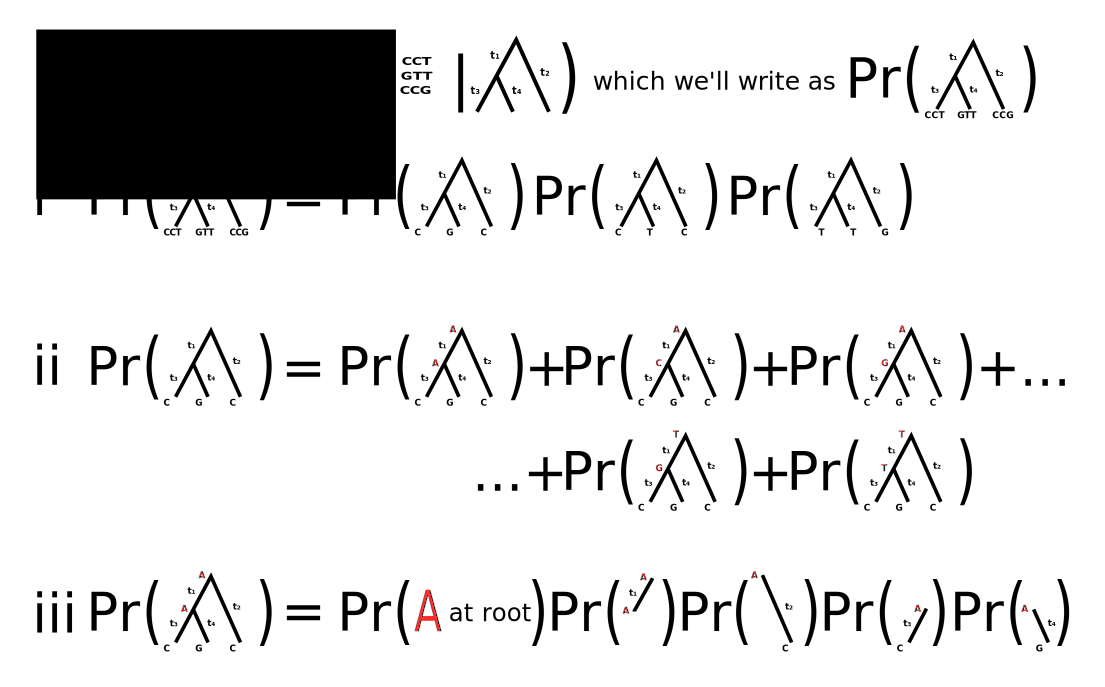
\includegraphics[width = 23cm, height = 13.7cm]{figures/treeprob.pdf}
\caption{A schematic representation of calculating the likelihood of a tree $P(D|T)$.  Equation i holds since each site (column of $D$) is assumed independent,  so $P(D|T) = \prod_{i = 1}^L P(D_i|T)$.  Equation ii expands the first term on the right of equation i.  It shows all possible ancestral values (shown in red) being summed over, $P(D_i|T) = \sum_{A_i} P(D_i, A_i|T)$.  The sum, here containing 16 terms,  can be efficiently calculated using dynamic programming. Equation iii expands the first term on the right of equation ii and relies on an assumption of independent evolution down different lineages.  The probability of the root value is given by the stationary distribution $\pi$, while the probability of having $X$ at the top of a lineage of length $t$ and $Y$ at the bottom is given by $P_{XY}(t) = [\exp{(tQ)}]_{XY}$.  So the right of equation iii equals the product $\pi_A P_{AA}(t_1)P_{AC}(t_2)P_{AC}(t_3)P_{AG}(t_4)$.}
\label{fig:treeprob}
\end{figure}
\end{landscape}



%The mutation of sequences does not influence the shape of the tree so long as mutations are {\em selectively neutral}, that is, the chance of an individual dying  or producing offspring is unaffected by the version of the gene it is carrying.  This is most easily seen in the Wright-Fisher context, where all sequences are expected to produce the same number of off-spring, the shape of the tree will be the same whatever the state of the sequences.    Typically we aim to work with relatively neutral regions of the sequence so that the assumption of neutrality is not too bad.

%Given this assumption, and the assumption that all individuals evolve independently and identically, we conclude that the mutation process will act similarly down all edges (branches) of the tree so we need only concern ourselves with how the mutation process works between arbitrary time points.    


 
 \subsection{Markov processes} \label{sec:markovpro}


%We model only the {\em substitution process} in which one base is replaced by another, for example $A \rightarrow T$ or $A \rightarrow C$.  We assume that all sites in a sequence behave in the same way and independently of each other, so we need initially only consider a single site which, assuming it a a DNA sequence, may take values $A,C,G,T$.


The model we use is a continuous time Markov model (often called {\em Markov processes}).  We haven't got time to go into this in much detail but the main idea behind it is relatively intuitive.  

We've already seen a simple Markov process, in the form of the Poisson process.  Recall that in the Poisson process, `events' can occur at any time, times between events are exponentially distributed and, in a very period of time, we expect either to see no events or one event (but not two or more). In the Poisson process, we only considered a single type of event and simply counted them when they occurred so that the state of the process was just a count of the number of things that had occurred so was strictly increasing.   

The model we use for mutations is similar to the Poisson process in that waiting times between events are exponential and, in a short slice of time, nothing or just one event will occur.  The events  are substitutions so we want to keep track of the state of the process at each time point.  Let $X(t)$ the  state of the process at time $t$ (so $X(t) \in \{A,C,G,T \}$).  The difference from a Poisson process is that we allow that the rate of different events occurring may be different.  For example, the rate of mutations  from state $A$ to state $G$ may be different from the rate at which $A$ mutates to $T$. 

Let $q_{ab}$ be the instantaneous rate of transitions from state $a$ to state $b$, for any states $a \neq b$.    It may help to think of this in terms of flow: $q_{ab}$ is the rate of flow form state $a$ to state $b$.

$q_{aa}$ is  the total rate of flow out of $a$, so it is the sum of rates from $a$ to $b$ for $b \neq a$ and is defined to be negative, $q_{aa} = - \sum_{a\neq b} q_{ab}$.  This means that the length of time spent in state $a$ is exponentially distributed with rate $-q_{aa}$.

Now define the rate matrix $Q$ to have off diagonal elements $q_{ab}$ and diagonal elements $q_{aa} = - \sum_{a\neq b} q_{ab}$.  



In the case of modelling DNA mutations, $Q$ has the form
 \[ Q = 
\renewcommand{\arraystretch}{1.25}
\left(  \begin{array}{cccc}
-\sum_{j \neq A}q_{Aj} & q_{AC} &  q_{AG} &  q_{AT} \\
q_{CA} & -\sum_{j \neq C}q_{Cj}  &  q_{CG} &  q_{CT}  \\
a_{GA} & q_{GC} & -\sum_{j \neq G}q_{Gj} &  q_{GT} \\
q_{TA} &  q_{TC} &  q_{TG} & -\sum_{j \neq T}q_{Tj} 
 \end{array} \right).\] 
 where $q_{ij}$, $i \neq j$ can be interpreted as the instantaneous rate that $i$ mutates to $j$. 


Now define $P_{ab}(t) = \Pr(X(t) = b|X(0) = a)$  the probability of starting in state $a$ at time 0 and being in state $b$ at time $t$ and form the matrix $P(t) = [P_{ab}(t)]$.  It turns out that we can derive $P(t)$ from $Q$ by taking the matrix exponential:
 \[ P(t) = \exp(Q t)  = \sum_{k = 0}^{\infty}  \frac{ (Q t)^k}{k!}.  \]
 
The matrix exponential can sometimes be calculated analytically but, for general $Q$, use numerical methods which are available for many standard numerical libraries.

%%\notinexam{
The matrix exponential follows the rules we would hope for the exponential function.  For example:
\begin{itemize}
\item $\exp(\mathbf 0) = \mathbf I_n$
\item when $\mathbf{AB} = \mathbf{BA}$, $\exp(\mathbf{A+B}) =\exp(\mathbf{A})\exp(\mathbf{B}) $
\item When $\mathbf B$ is invertible, $\exp(\mathbf{BAB}^{-1}) = \mathbf{B}\exp(\mathbf{A})\mathbf B^{-1}$
\item If $\mathbf A = \mathrm{diag}(a_1,\ldots,a_n)$, then $\exp(\mathbf A) = \mathrm{diag}(\exp(a_1),\ldots,\exp(a_n))$.
\end{itemize}
%%}%end not in exam
 
  
\subsection{Models of sequence mutation}


There are a lot of parameters to specify or estimate in a full model of sequence mutation: on the face of it, we need to specify each of the $q_{ab}$s (giving us 12 parameters when there are 4 bases).  In reality, we make various simplifying assumptions to reduce the number of parameters and make estimation simpler.

% The wiki page \url{http://en.wikipedia.org/wiki/Models_of_DNA_evolution} has a good summary of the different models.

We insist that models of mutation are {\em reversible} and {\em stationary}.

A process is stationary when , if run for long enough, it settles down to some equilibrium,  $\pi = \left[ \pi_A, \pi_C, \pi_G, \pi_T \right]$.  Formally, $\pi$ is defined by the equation $\pi P(t) = \pi$ for any $t$.   That is, if the process starts in equilibrium, running the process further will leave it in equilibrium.  $\pi$ is called the equilibrium distribution or the stationary distribution.  

A  process is reversible when it looks the same running backwards as it does running forwards.    Strictly, a process is reversible when it satisfies the detailed balance conditions $\pi_i p_{ij}(t) = \pi_j p_{ji}(t)$ for all values of $i, j$ and $t$.

It helps when specifying substitution matrices to normalise them so that the average number of mutations per unit time is one. Given an unnormalised matrix $\hat Q$, it can be normalised by multiplying  each entry by some constant $\beta$, so that the normalised matrix is $Q = \beta \hat Q$.  The value of $\beta$ depends on $\hat Q$.

Scaling the substitution matrix in this manner means that time is measured in substitutions.  That is, one time unit corresponds to the time in which we would expect to see one mutation at any given site. 



\subsection*{Summary of assumptions we make}

\begin{itemize}
 \item   Each site is identical to all others in the evolutionary processes operating on it.
\item    Each site is free to change independently of all other sites.
\item    These two assumptions are usually stated as sites are independent and identically distributed, or i.i.d.
\item    Substitution probabilities do not change with time or over the tree. This is known mathematically as a homogeneous Markov process.
\item    The mutation process is time-reversible meaning that the process looks the same whether it is run forward or backward in time.
\item Mutation process are independent across across different branches.
\end{itemize}

So given a mutation model (that is, given $Q$ and $\mu$), we can easily determine the probability of observing a descendant sequence given an ancestral sequence.  For example, given the sequence $x_1 = ACTT$ at time $t_1$ and the $x_2 = AGGT$ at time $t_2$ and assuming 

%\tikzset{vertex/.style = {circle, draw, fill=black!50,inner sep=0pt, minimum width=4pt}}
%\tikzset{point/.style = {inner sep=0pt, minimum width=0pt}}
%\begin{tikzpicture}[thick,y=6cm,x = 2cm]
%    \node [vertex,label = below:  $x2=AGGT$] at (0,0) (x) {} ;
%    \node [vertex,label = below:  $x1=ACTT$] at (0,3) (y) {} ;
%     \path (x) edge (y);
%\end{tikzpicture}
%
\begin{tikzpicture}[thick]
    \node [vertex] at (0,0) (x2) {} ;
    \node [below of = x2,node distance = 4mm,label = above right:  $t_2$]  {$x_2 = AGGT$};
    \node [vertex] at (0,3) (x1) {} ;
    \node [above of = x1,node distance = 4mm,label = below right:  $t_1$]  {$x_1 = ACTT$};
              
    \path (x1) edge  (x2);
\end{tikzpicture}\\

But given a tree with samples at the tips, the ancestral sequences are unknown to us.  But how does this work when we don't know the ancestral sequences?  We need to sum over all possible ancestral sequences. It turns out that this is relatively easy to achieve using a dynamic programming approach known as Felsenstein's peeling (or pruning) algorithm (1981) which performs this calculation in polynomial time based on a post-order traversal of the tree.  We omit the details.



\subsubsection{Jukes-Cantor model}

 The simplest model  is the {\em Jukes-Cantor} model  (1969) which has equal rates of mutation between all bases so that  $q_{ij} = 1$ for $i \neq j$, 
   \begin{equation*}
Q = \beta \begin{bmatrix}
-3 & 1 & 1 & 1 \\
  1 & -3 & 1 & 1 \\
  1  & 1  &  -3 & 1  \\
  1 & 1 & 1 & -3
 \end{bmatrix}.
\end{equation*}
In this case, $\beta = 1/3$ so 
   \begin{equation*}
Q =  \begin{bmatrix}
-1 & 1/3 &  1/3  &  1/3  \\
   1/3  & -1 &  1/3  &  1/3  \\
   1/3   &  1/3   &  -1 &  1/3   \\
   1/3  &  1/3  &  1/3  & -1
 \end{bmatrix}.
\end{equation*}
The equilibrium of this process is  $\pi = (1/4,1/4,1/4,1/4)$.  

The transition matrix $P(t) = \exp(Qt)$ for the Jukes-Cantor model  has off-diagonal entries
\[P_{ij}(t) = \frac14 - \frac14 \exp\left( - t \mu\right)\] and diagonal entries
\[P_{ii}(t) = \frac14 + \frac34 \exp\left( - t \mu\right).\] 

%%\notinexam{
\subsubsection{Kimura model}

The Kimura model (1980) distinguishes between {\it transitions} ($A \longleftrightarrow G$ and $C \longleftrightarrow T$ state changes) and {\it transversions} (state changes from a  purine to pyrimidine or {\it vice versa}). 
The model assumes base frequencies are equal for all characters.
This transition/transversion bias is governed by the $\kappa$ parameter and the $Q$ matrix is:


  \begin{equation*}
Q =  \beta \begin{bmatrix}
-2-\kappa & 1 & \kappa & 1 \\
  1 & -2-\kappa & 1 & \kappa \\
  \kappa & 1  &  -2-\kappa & 1  \\
  1 & \kappa & 1 & -2-\kappa
 \end{bmatrix},
\end{equation*} 

The normalized $Q$ is obtained by setting $\beta = \frac{1}{2+\kappa}$. This model has one free parameter, $\kappa$. The transition probabilities are:

\begin{equation*}
p_{ij}(d) =  \begin{cases}
\frac{1}{4} + \frac{1}{4} \exp(-\frac{4}{\kappa+2}d) + \frac{1}{2}\exp(-\frac{2\kappa+2}{\kappa+2}d) & \text{if } i=j\\
\frac{1}{4} + \frac{1}{4} \exp(-\frac{4}{\kappa+2}d) - \frac{1}{2}\exp(-\frac{2\kappa+2}{\kappa+2}d)  &  \text{if transition}\\
\frac{1}{4} - \frac{1}{4} \exp(-\frac{4}{\kappa+2}d) &  \text{if transversion}
   \end{cases}.
\end{equation*} 


\subsubsection{F81 and HKY models}
In 1981, Joe Felsenstein proposed a model that extends the Jukes-Cantor model to allow for unequal equilibrium base frequencies, that is $\pi$ for which $\pi_a \neq \pi_b$. This is known as the F81 model.  The F81 model has 3 parameters, one less than the number of equilibrium base frequencies since there is the restriction that $\sum_i \pi_i = 1$.

In 1985, the F81 model was extended to incorporate the Kimura model, so  allows different rates for transitions and transversions as well as unequal base frequencies.  The resulting model is known as the HKY model and has rate matrix of the form:
 \begin{equation*}
Q = \beta \begin{bmatrix}
\cdot & \pi_C & \kappa\pi_G & \pi_T \\
  \pi_A & \cdot & \pi_G & \kappa\pi_T \\
  \kappa\pi_A  & \pi_C  &  \cdot & \pi_T  \\
  \pi_A & \kappa\pi_C & \pi_G & \cdot
 \end{bmatrix}
\end{equation*}
where the diagonal elements are defined in the usual way so that the row sums are zero.  The transition matrix $P$ can be calculated analytically for this model but it is omitted here.

\subsubsection{GTR model}

In 1986, the most general reversible model was developed which can have an arbitrary stationary distribution, and given the restriction of reversibility, 6 parameters for adjusting the rates of mutation between bases.  The rate matrix is 
 \[ \renewcommand{\arraystretch}{1.25}
Q = \beta \left[  \begin{array}{cccc}
- & a\pi_C & b\pi_G & c\pi_T \\
a \pi_A  & - & d\pi_G & e\pi_T \\
b \pi_A &  d\pi_C & - & f\pi_T\\
c \pi_A &  e\pi_C & f\pi_G & -
 \end{array} \right].\] 
 
    The diagonal elements are calculated in the normal way.  
 
 Where the normalization is $\beta = 1/[2(a\pi_A\pi_C+b\pi_A\pi_G+c\pi_A\pi_T+d\pi_C\pi_G+e\pi_C\pi_T+\pi_G\pi_T)]$

    
This model has 9 parameters to be specified: the parameters of the equilibrium distribution,
  $\pi = (\pi_A,\ldots,\pi_T)$,  (since $\sum_i \pi_i = 1$, this only counts for 3 parameters) and the parameters $a,b,c,d,e,f > 0$.
    Note the form of the $Q$ matrix here is chosen so that $\pi$ is indeed the equilibrium distribution, that is, as $t \rightarrow \infty $, every row of $P(t) \rightarrow \pi $.  
    Recall that $P(t) = \exp( t Q )$, where $\exp()$ is the matrix exponential.   
 
The same modelling tools can be used when the bases are the 20 amino acids, the difference being that the $Q$ matrix is now $20\times20$.



\subsubsection{Rate variation across sites}

An obvious property many  real alignments share is that different sites (i.e., columns) in the alignment appear to mutate at different rates: some sites appear to essentially be at equilibrium (so bases in that column are close to what you would expect if they were randomly drawn from the stationary distribution) while other sites may be constant.  

To account for this, multiply the rate matrix for each site by some multiplier $r_i$, $i = 1,\ldots, L$, where $L$ is the number of sites.  Typically, the $r_i$s are modelled as coming from a gamma distribution with mean 1 and variance determined by the shape parameter $\alpha$.  To simply computation, the gamma distribution is discretised into $K$ categories (that is, it is approximated by a discrete distribution taking $K$ possible values), so that $r_i$ can only take one of $K$ possible values.  The $r_i$ are known as relative rates.  Seeing the mean of the $r_i$s is 1, the expected number of mutations per unit time per site is still 1.

Finally, the constant sites in the alignment can be dealt with directly by allowing the the relative rate to be zero at those sites.

The shorthand used for these models is, for example, GTR+$\Gamma$+I, meaning that the general time reversible model is used with rate variation treated under the (discrete) gamma model with invariant sites allowed for.  
%%} %end not in exam



 
 \subsection{Estimating the maximum likelihood tree}
 
According to the substitution model we are using, the best tree is the one which maximises the likelihood $\mathcal L(T) = \Pr(D|T)$ under that model.  This is called the maximum likelihood tree.     Since there is no way to analytically find the maximum likelihood tree under general model of mutation,   we can use similar techniques to those used for maximum parsimony to find something close to the maximum likelihood tree.   

That is, we can start at some tree and use a stochastic search to propose new trees which are accepted if they have a higher likelihood. Note that we have the added complication when dealing with likelihoods that branch lengths now influence the likelihood of a tree, so for each tree topology, the branch lengths need to be optimised.
 
The hill-climbing algorithm we introduced in the context of parsimony trees is restated here for likelihood trees:

\begin{itemize}
\item    choose an initial tree and calculate its likelihood.
  \item Iterate: \begin{itemize} \item modify the tree and calculate its likelihood.
  \item  if the modified tree has a higher likelihood then the unmodified tree, keep it. Else, return to the previous tree
  \item  stop when no or minimal increase in likelihood occurs
\end{itemize}
\end{itemize}

Modifications to the tree can either change the tree topology (shape) or the length of the branches.  The same topology changing operations as we used in the equivalent parsimony algorithm,  such as SPR, can be  extended to work with trees with explicit branch lengths as we have here.  Modifications that change only the branch lengths are also used in this context.
 
 
 \subsection{Bayesian approach to phylogenetics}
 
 What we really want is not just the likelihood, but the posterior probability of the tree (and other model parameters) given the data.  That is, given data $D$ we want to find the posterior distribution $P(g,Q,\mu |D)$.  From Bayes' Theorem, 
 \[  P(g,Q,\mu |D) = \frac{P(D|g,Q,\mu)P(g,Q,\mu)}{P(D)} \]
 where $P(D|g,Q,\mu)$ is the likelihood for the parameters with fixed data, $P(g,Q,\mu)$ is the prior distribution for the parameters and $P(D)$ is a normalisation constant.  
 
 Once again, we are unable to calculate this analytically so resort to numerical techniques to study this object.  The primary computational tool that is used in Bayesian phylogenetics is Markov chain Monte Carlo (MCMC).  MCMC gives us a method of generating samples from the posterior distribution.  These samples form the basis of our investigation of the posterior distribution.


 \subsection{Models for trees: Yule trees and the coalescent}
 
 We look at two basic models for trees, the Yule tree and the coalescent.  Yule trees are typically used when we have observed sequences from multiple different species.  It models speciation as rare, random events.   The coalescent is used to model trees when all sequences came from the same population and species.  It is based on a model of how individuals in a population interact. 
  
 \subsubsection{Yule trees}
 
A Yule tree can be viewed as a realisation of  the Yule process which is a pure both process.  It starts at time $t_0 = 0$ with one lineage (species).  Each lineage branches according  to a Poisson process with rate $\lambda$.  That is, a lineage branches after some time $t \sim Exp(\lambda)$.  When a lineage branches it produces an exact copy of itself that proceeds in the same way and will go on to branch according to this same process.  Here, branching model speciation events, where all species are equally likely to speciate.  

So when there are $k$ lineages, branching occurs at according to Poisson process with total rate $k\lambda$.  

We usually ignore the branch above the root, so start the process with $k=2$.  So to simulate the Yule process, set $k=2$ and $t= 0$ and make a root node at time $t$ with two lineages. Iterate:  Draw $t_k \sim Exp(k\lambda)$ and set $t = t+t_k$.  Pick one of the lineage uniformly at random by copying it by making a node with time $t $ and two children. Increment $k$.  

To produce a tree with $n$ leaves, stop the process immediately before the $n+1$th lineage is produced (at time $\sum_{k = 2}^n t_k$.  

We could have produced this tree in reverse by starting with $n$ leaf nodes and $n$ lineages above them. Let $k = n$. Simulate a time $t_k \sim Exp(k\lambda)$ and set $t= t+t_k$. Choose a pair of lineages uniformly at random.  Make a node at time $t$ with these two chosen lineages as children.  Decrement $k$. Stop when $k=1$.

Given a tree, $g$, that was produced according to this process we can write down the probability density of this tree. Label the nodes with time increasing back into the past, so leaf nodes to have time $t_n = 0$ and node $k$ has time $t_k$ and there are $k$ lineages between time $t_k$  and $t_{k-1}$.  Then the probability density function of a tree, given the branching rate $\lambda$ is, 
\[ f(g|\lambda)  = \prod_{k=2}^n  \lambda \exp\left(-k\lambda (t_{k-1} -t_k)\right).  \]

\subsubsection{The coalescent}
 
 The coalescent comes from considering how two individuals in a simple population are related.  The population is modelled by one of the simplest models of a interacting population used in population genetics, known as the Wright-Fisher model.  The Wright-Fisher model has a constant size population consisting of $N$ individuals and generations are discrete.  All individuals are equally likely to produce offspring in the next generation.  That is, at the end of a generation, the whole current population dies and is replaced by their offspring.
 
 This can be modelled as thinking of each of the $N$ offspring in the $(k+1)$th generation choosing a parent uniformly at random from the $k$th generation (that is, the previous generation).  So, on average, each individual in the $k$th generation has one child surviving in the $k+1$th generation but some will have $0, 1, 2,$ etc. 
 
 The coalescent comes about by considering the process going backward in time and asks, if we choose two individuals in the current generation uniformly at random, who many generations do we have to go back until this pair shares a common ancestor?
 
The chance that they share an ancestor in the previous generation is simply that the probability that they share a parent, which has probability $1/N$ (recall that $N$ is the population size), while the probability they do not share a parent is $1- 1/N$.  If they don't share a parent, the same argument holds for each preceding generation: they share a parent with probability $1/N$ and not with probability $1-1/N$.  When the pair share a parent, we say that they `coalesce' in the parent generation. Let $T$ be the number of generations back to coalescence.  Then
\[ \Pr(J = j) = \frac 1N \left(1-\frac 1N \right)^{j-1}\]
which is just a geometric distribution.  So the expected time to coalescence is $N$ generations.  It is natural to chose a time scale so that one time unit is $N$ generations and consider the limit as $N$ gets large.  

So set $t = \frac j N$ where $j$ is time measured in generations.  Now, $j = tN$
Then the probability that the two lineages have not coalesced in $t$ time units is 
\[ \left(1-\frac1N \right)^{tN -1} \longrightarrow e^{-t} \mbox{ as } N \rightarrow \infty. \]
That is, the expected time to coalescence for a pair of individuals in a large population is exponentially distributed with parameter 1.  The result is true for any pair, so if we choose $k$ indidividalusl and trace their ancestry back, each pair coalesces at rate 1 and, since there are ${k \choose 2}$ pairs, coalesences occur at total rate  ${k \choose 2}$ (that is the first coalescence between some pair will occur after an exponentially distributed time with parameter ${k \choose 2}$).  Remember that time was scaled so that 1 time unit was equal to $N$ generations, so the time to coalescence is proportional to the population size.

Thus we have a method of simulating coalescent trees.
\begin{enumerate}
\item Set $k = n, t = 0$.  
\item Make $n$ leaf nodes with time $t$.  This is the set of available nodes.
\item While $k \geq 2$, iterate:
\item Generate a time $t_k \sim \mbox{Exp}( {k \choose 2})$. Set $t = t + t_k$.
\item Choose two nodes uniformly at random  and let them coalesce at a new node with time $t$. Replace the two chosen nodes in the set of available nodes with this new node.
\item Set k = k-1.
\end{enumerate}


A coalescent tree reflects the ancestry of a sample of $n$ individuals drawn from a large population of $N$.  


It is often convenient to measure time in units of expected mutations.  Consider a Wright-Fisher model in which mutations occur with probability $u$ at each generation.  That is, there is a probability $u$ that  an individual differs from its parent by a single mutation.  Let $\theta = 2Nu$, so $\theta$ is the expected number of mutations separating 2 sequences (since there are $N$ generations back to a common ancestor, on average, each lineage picks up $Nu$, so there are a total of $2Nu$ mutations between the two lineages).  

So if we want to define time in units of expected number of mutations, we multiply coalescent time (which is measured in units of $N$ generations) by $\frac {\theta}2$, that is multiple all branch length by $\frac{\theta}{2}$.   So instead of a rate of coalescence of $1$ for each pair, we have a rate of coalescence of $\frac 2{\theta}$ for each pair (recall that the mean of an exponential is $1/\mbox{rate}$, so mean time to coalescence for a pair with rate $\frac{2}{\theta}$ is $\frac{\theta}{2}$).

The total coalescence rate when there are $k$ lineages is thus \[ \frac{2}{\theta} {k \choose 2} = \frac{2}{\theta} \frac{k(k-1)}{2} = \frac{k(k-1)}{\theta}.\]


The density for a coalescent tree is similar to that of a Yule tree.  With a coalescing rate of $\frac{2}{\theta}$, the density is 


\[ f(g|\theta)  = \prod_{k=2}^n  \frac{2}{\theta} \exp(-\frac{ k(k-1)}{\theta} (t_{k-1} -t_k)).  \]

 
 Note that different time scales may be encountered in the literature: actual calendar time, time scaled so that $N$ generations passes in 1 time unit, time scaled so that $2N$ generations passes in 1 time unit (to account for the fact that in a diploid population of N individuals, there are $2N$ copies of every gene)  or evolutionary time where $\theta$ is the time unit.  
 
 
\subsubsection{Properties of the coalescent}

Let $H_n$ be the height of a coalescent tree with $n$ leaves, then \[ E(H_n) = 2\left(1 - \frac1n\right).\]

Let $L_n$ be the total length of a coalescent tree with $n$ leaves.  Then \[E(L_n) = 2 \sum_{k= 1}^{n-1} \frac 1 k \approx 2 \log(n).\]

 
 \end{document}
 
 
 \section{Sampling from an unknown distribution}
 \begin{itemize}
 \item MCMC recap
 \item what to do with samples: estimating means and the variance of those estimates: 
 \item How many samples do we have?
 \
\end{itemize} 
 
 
 \section{Summarising distributions of trees}
 
 This section from Andrew Rambaut \url{http://beast.bio.ed.ac.uk/summarizing-posterior-trees}
 
There are many ways to summarize the posterior distribution of tree topologies and branch lengths. Here I outline a few options:
50\% Majority consensus tree and extended majority consensus tree

The 50\% majority consensus tree is a tree constructed so that it contains all of the clades that occur in at least 50\% of the trees in the posterior distribution. In other words it contains only the clades that have a posterior probability of >= 50\%. The extended majority tree is a fully resolved consensus tree where the remaining clades are selected in order of decreasing posterior probability, under the constraint that each newly selected clade be compatible with all clades already selected. It should be noted that it is quite possible for the majority consensus tree to be a tree topology that has never been sampled and in certain situations it might be a tree topology with relatively low probability, although it will have many features that have quite high probability.
'Maximum clade credibility tree'

A natural candidate for a point estimate is the tree with the maximum product of the posterior clade probabilities. To the extent that the posterior probabilities of different clades are additive, this definition is an estimate of the total probability of the given tree topology (i.e. it provides a way of estimating the maximum a posteriori tree topology, see below).

\subsection{MAP tree}

The use of the term MAP tree has been often misused in the literature. It has sometimes been used to describe the tree associated with the sampled state in the MCMC chain that has the highest posterior probability density. This is problematic, because the sampled state with the highest posterior probability density may just happen to have extremely good branch lengths on an otherwise fairly average tree topology. A better definition of the MAP tree topology is the tree topology that has the greatest posterior probability, averaged over all branch lengths and substitution parameter values. For data sets that are very well resolved, or have a small number of taxa, this is easily calculated by just determining which tree topology has been sampled the most often in the chain. However for large data sets it is quite possible that every sampled tree has a unique topology. In this case, the alternative definition of maximum clade credibility tree above can be used.
Median tree

To define a median tree, you must first define a metric on tree space. This turns out to be quite a difficult thing to do, but there are number of candidate metrics described in the literature. If you can visualize the trees in your posterior sample as a cluster of points in a high-dimensional space, then the median tree is the tree in the middle of the cluster - the median tree has the shortest average distance to the other trees in the posterior distribution. With a metric defined (say the Robinson-Foulds distance), a candidate for the median tree would be the tree in your posterior sample that has the minimum mean distance to the other trees in the sample. (see \url{http://en.wikipedia.org/wiki/Geometric_median}).
95\% Credible Set

For data sets that are very well resolved, you might consider reporting not a single tree, but the smallest set of all tree topologies that accounts for 95\% of the posterior probability. This is known as the 95\% credible set of tree topologies. 

The Maximum Credible Tree criterion could also be used to obtain an approximate x\% credible set for small x.


\subsection{Divergence times }

Once you have the decided on the tree topology or topologies that best summarize(s) your Bayesian phylogenetic analysis, the next question is what divergence times (node heights) to report. One obvious solution is to report the mean (or median) node height for each of the clades in the summary tree. This is especially suitable for the majority consensus tree and the maximum credibility tree (however defined). For the median tree, it should be noted that some metrics (i.e. those that take account of branch lengths and topology) allow for a single tree in the sample to be chosen that has the median topology and branch lengths. Likewise, if the 'MAP' sampled state is the chosen tree topology, then the associated branch lengths of the chosen state can be reported.

It should be noted that for a given topology, the mean height of a node could be older than its ancestor's mean height resulting in negative branch lengths. 

 \section{Choosing prior distributions}
 
 The prior distribution should, in theory summarise exactly exactly what we know about the parameters before seeing the data.
 
 In practice, this can be difficult as there are often different types of knowledge we want to include in the prior or we may just want to express our ignorance.  In either case, deciding on the correct functional form to express our state of knowledge is difficult.
 
 A good guiding principle is that the prior should be constructed in such a way that it gives equal weight to different hypotheses we are testing.  For example, suppose we are trying to estimate the age of a clade in a tree and everyone agrees that the clade is between 0 and 10m years old.    Suppose further that the there are two competing hypotheses: one that the true age is between 0 and 2m years, the other that is between 2m and 10m years.    If we chose a uniform prior, for example, on 0 to 10m years, we would be giving 20\% of the prior weight to hypothesis 1 but 80\% of the prior weight to hypothesis 2, clearly giving an unfair advantage to hypothesis 2.  A fairer prior would be to place 10
 
 Priors are often used to express ignorance: typical parametric forms include uniform priors, $1/x$ priors, normal or log-normal priors.  Whether or not those are informative depends on the type of variable we are looking at.  An important distinction to make is location and scale parameters.  
 
 Scale parameters refer to the spread of distribution, how wide it is.  Variances, standard deviations and rates are scale parameters.  
 
 Location parameters refer to where the centre of the distribution is: positions, dates, means, medians and modes are typical location parameters.
 
 
 
in complex models, we nearly always assume, a priori, that the parameters are independent, and we specify them in that way.  For example, if we have two parameters to estimate, $\mu$ and $\lambda$, assume independence between them so that the prior $f(\mu,\lambda) = f(\mu)f(\lambda)$.  However, it can be difficult to know how various priors interact: for example, if we set a coalescent prior for the tree and then constrain certain nodes, what does that prior 

\section{Posterior predictive estimation}




\section{Estimating population sizes}
 
\end{document}

 
 %%%%%%%%%%%%%%%%%%%%%%%%%%
%%%%%%%%%%%%%%%%%%%%%%%%%%
%%%%%%%%%%%%%%%%%%%%%%%%%%
%%%%%%%%%%%%%%%%%%%%%%%%%%
%%%%%%%%%%%%%%%%%%%%%%%%%%
%%%%%%%%%%%%%%%%%%%%%%%%%%
\end{document}
%%%%%%%%%%%%%%%%%%%%%%%%%%
%%%%%%%%%%%%%%%%%%%%%%%%%%
%%%%%%%%%%%%%%%%%%%%%%%%%%
%%%%%%%%%%%%%%%%%%%%%%%%%%
%%%%%%%%%%%%%%%%%%%%%%%%%%
%%%%%%%%%%%%%%%%%%%%%%%%%%
%%%%%%%%%%%%%%%%%%%%%%%%%%








